\documentclass[a4paper,12pt]{scrreprt}

    %% Used for changing geometry of the page
    %% Cover page text cannot overlay cover sketching/style 
    %% https://ctan.org/pkg/geometry?lang=en
\usepackage[portuguese]{babel}
\usepackage{ltablex}
\usepackage{booktabs}
\usepackage{array}
\keepXColumns
\usepackage{geometry}
\usepackage{graphicx} % O pacote correto para imagens
\usepackage{tabularx}
\usepackage{ragged2e} % Para um texto mais bonito em colunas estreitas
\usepackage{float}
\usepackage[round]{natbib} % Estilo de citação com parênteses
\bibliographystyle{plainnat} % Um dos estilos compatíveis com Harvard
\usepackage{enumitem}
\usepackage{longtable}

    %% Changes language of some packages protocols
    %% e.g., when captioning images: Figure 1. -> Figura 1.
    %% https://ctan.org/pkg/babel?lang=en
    %% Used for special fonts
    %% Cannot be compiled with pdflatex
    %% https://ctan.org/pkg/fontspec?lang=en
\usepackage[utf8]{inputenc} % Permite acentos
\usepackage[T1]{fontenc}    % Melhor codificação de fonte
\usepackage{helvet}         % Carrega a fonte Helvetica (clone da Arial)
\renewcommand{\familydefault}{\sfdefault} % Define como fonte padrão

    %% More colors and color options
    %% https://ctan.org/pkg/xcolor?lang=en
    %% https://ctan.org/pkg/colortbl?lang=en
\usepackage{xcolor,colortbl}

    %% More tabular options, like dashed/dotted lines
    %% https://ctan.org/pkg/arydshln?lang=en
\usepackage{arydshln}
\usepackage{listings}
\usepackage{xcolor}

\lstset{
    basicstyle=\ttfamily\small,
    breaklines=true,
    frame=single,
    extendedchars=true,         % Permite caracteres estendidos
    literate=
        {á}{{\'a}}1 {ã}{{\~a}}1 {â}{{\^a}}1 {à}{{\`a}}1
        {é}{{\'e}}1 {ê}{{\^e}}1
        {í}{{\'i}}1
        {ó}{{\'ó}}1 {õ}{{\~o}}1 {ô}{{\^o}}1
        {ú}{{\'u}}1
        {ç}{{\c{c}}}1
        {Á}{{\'A}}1 {Ã}{{\~A}}1 {Â}{{\^A}}1 {À}{{\`A}}1
        {É}{{\'E}}1 {Ê}{{\^E}}1
        {Í}{{\'I}}1
        {Ó}{{\'O}}1 {Õ}{{\~O}}1 {Ô}{{\^O}}1
        {Ú}{{\'U}}1
        {Ç}{{\c{C}}}1
}

    %% List of acronyms
    %% https://ctan.org/pkg/nomencl?lang=en
\usepackage[intoc]{nomencl}
    %% Must be called to init nomencl environment  
    \makenomenclature

    %% More images options/settings
    \graphicspath{{images/}} 
    
    %% used to handle cross-referencing commands in LaTeX to produce hypertext links in the document
    %% https://ctan.org/pkg/hyperref?lang=en
\usepackage{hyperref}
    
%% settings
    \hypersetup{
        colorlinks,
        citecolor=black,
        filecolor=black,
        linkcolor=black,
        urlcolor=black
    }

\usepackage{amsmath}
    %% Defining backgrouns, used to make the cover
    %% https://ctan.org/pkg/background?lang=en
\usepackage[some]{background}
    %% Used to make drawings or complex graphics
    %% http://pgf.sourceforge.net/pgf_CVS.pdf
\usepackage{tikz}
    %% Tikz library to point operations ((x1,y1) + (x2,y2))
    \usetikzlibrary{calc}

%% Defining sfdefault font and default font for document
\renewcommand{\familydefault}{\sfdefault}

%% Costume made cover 
%% From there you can use \makecover command to build the cover
\include{cover}

%==========================================================================
% DOCUMENT
%==========================================================================

\begin{document}

\pagenumbering{gobble}

% builds the cover
\makecover

%% smaller footer and header size
\newgeometry{top=3cm,left=3cm,right=3cm,bottom=4cm}

%% Abstract name: \Large font size, flushed left and paragraph skip before abstract content
\renewenvironment{abstract}
 {\par\noindent\textbf{\Large\abstractname}\par\bigskip}
 {}

\begin{flushleft}
\begin{abstract}
   O presente relatório detalha a primeira fase de desenvolvimento do sistema Fix'n'Ride, uma solução de gestão integrada concebida para a oficina de micromobilidade elétrica MobiFix. No contexto atual de expansão das Smart Cities, a digitalização dos serviços de assistência técnica tornou-se um imperativo estratégico para superar a ineficiência dos processos manuais e a fragmentação de dados em folhas de cálculo. Esta etapa inicial focou-se primordialmente na engenharia de requisitos e na modelação conceptual do sistema. O levantamento de necessidades foi realizado através de uma abordagem mista, integrando questionários, observação direta e entrevistas estruturadas com os principais stakeholders: administração, técnicos e operadores de loja. Deste processo resultou a especificação detalhada de 24 requisitos funcionais e 5 requisitos não funcionais, garantindo a cobertura de todo o fluxo operacional. O sistema permite a gestão integral de ordens de serviço baseadas num catálogo de intervenções com preços fixos, assegurando transparência orçamental ao cliente e eficiência na faturação. Adicionalmente, a solução engloba a gestão de inventário com alertas automáticos de stock mínimo, portais de agendamento online e dashboards de reporte financeiro. Ao nível da modelação, utilizou-se a linguagem UML para o desenho do Modelo de Domínio, a especificação detalhada de Casos de Uso, a realização de Diagramas de Atividades e de Máquinas de Estado, estabelecendo as bases lógicas para a futura implementação. A arquitetura tecnológica assenta na plataforma .NET, React.js e SQL Server, privilegiando a robustez e a responsividade em múltiplos dispositivos. Destaca-se ainda a utilização de Grandes Modelos de Linguagem (LLMs) como agentes auxiliares na aceleração das fases de conceção, codificação e documentação, otimizando o ciclo de vida do software. O trabalho realizado nesta etapa garante a viabilidade técnica e operacional necessária para a sustentabilidade económica da MobiFix. \par \textbf{Área de Aplicação}: Engenharia de Software, Sistemas de Informação, Gestão de Oficinas. \par \textbf{Palavras-Chave}: LLM, .NET, C\#, SQL, UML, Gestão de Reparações, Bases de Dados Relacionais, Inteligência Artificial Generativa. \end{abstract}
\end{flushleft}

\pagebreak

%==========================================================================
% BEGIN INDEXES PAGES
%==========================================================================

\renewcommand{\contentsname}{Índice}
\tableofcontents
\pagebreak
\listoffigures
\pagebreak
\listoftables
\pagebreak

%==========================================================================
% BEGIN INTRODUCTION
%==========================================================================

\pagenumbering{arabic}
\chapter{Introdução e apresentação do trabalho}

\section{Contextualização}
Na última década, o paradigma da mobilidade urbana sofreu uma transformação profunda e acelerada. A crescente pressão pela descarbonização dos transportes e a saturação das infraestruturas rodoviárias tradicionais impulsionaram a micromobilidade elétrica — com destaque para as trotinetes e bicicletas elétricas — para o centro das estratégias de desenvolvimento das \textit{Smart Cities}. O que começou como uma tendência de lazer consolidou-se como um pilar essencial do transporte quotidiano "last-mile", gerando um ecossistema global de veículos elétricos ligeiros que exige, agora, uma infraestrutura de suporte técnico igualmente evoluída. Contudo, esta expansão física e operacional não foi acompanhada por uma digitalização proporcional no setor dos serviços de assistência técnica. Muitas organizações, ao tentarem escalar as suas operações para responder a este volume massivo de procura, encontram-se limitadas por métodos de gestão tradicionais e sistemas de informação fragmentados. O software, neste contexto, deixou de ser um mero utilitário administrativo para se tornar no orquestrador central de sistemas dinâmicos, em evolução contínua e fortemente orientados a dados. Paralelamente, a própria Engenharia de Software atravessa uma revolução impulsionada pela Inteligência Artificial. A emergência dos \textit{Large Language Models} (LLM) alterou os métodos de idealização e desenvolvimento, permitindo que estes modelos atuem como agentes ativos em tarefas complexas, desde a Engenharia de Requisitos até à definição arquitetural. O presente trabalho insere-se na interseção destas duas realidades: a necessidade crítica de digitalização eficiente num setor de mobilidade em expansão e a utilização de agentes artificiais para acelerar e otimizar o ciclo de vida do software. 

\section{Motivação e Objetivos}
A motivação primordial para o desenvolvimento do sistema \textit{\textbf{Fix'n'Ride}} reside na urgência de dotar a MobiFix de uma infraestrutura tecnológica capaz de sustentar o seu crescimento acelerado. A atual dependência de processos manuais, como folhas de cálculo desconexas e registos em papel para a abertura de ordens de serviço, e a inexistência de uma visão integrada dos dados operacionais criaram um teto de vidro na escalabilidade da empresa, onde o aumento do volume de clientes deixou de se traduzir num aumento proporcional de lucro, resultando em desorganização e desperdício de recursos. A transição de uma gestão reativa para uma abordagem proativa e baseada em dados é o motor central deste projeto, visando eliminar custos ocultos e transformar a eficiência operacional numa vantagem competitiva. Neste âmbito, o projeto foca-se em atingir objetivos estratégicos claros, começando pela gestão eficiente do \textit{stock} e redução de capital imobilizado. Através da implementação de algoritmos de gestão de inventário para peças, prevê-se uma redução de 15\% nos custos de armazenamento e a eliminação de perdas por obsolescência. Simultaneamente, a digitalização do fluxo de trabalho técnico visa otimizar o ciclo de reparação (\textit{lead time}), projetando um aumento de 25\% na capacidade produtiva da oficina ao fornecer acesso imediato a históricos e manuais técnicos. No plano comercial, o desenvolvimento de um catálogo digital integrado pretende captar receita fora do horário físico, estimando-se um incremento de 20\% na faturação de componentes no primeiro ano. Por fim, a melhoria da experiência do cliente será assegurada por sistemas de notificação e acompanhamento automáticos, visando reduzir em 40\% o volume de contactos para ponto de situação, libertando recursos humanos e aumentando a taxa de fidelização através de uma maior transparência no serviço. 

\section{Apresentação do Caso de Estudo}
A \textit{\textbf{MobiFix -- Mobility Repair Services}} atua no setor da assistência técnica especializada de micromobilidade urbana, operando com um modelo de negócio inspirado nas redes multimarca automóveis, mas adaptado às especificidades de trotinetes. O crescimento exponencial da procura transformou a organização num centro de serviços de alto débito, processando atualmente um volume massivo de peças e de trotinetes de fabricantes como Xiaomi, Segway ou Ninebot, como com intervenções que variam entre a manutenção preventiva e diagnósticos eletrónicos complexos em componentes críticos. No entanto, a escalabilidade deste modelo encontra-se gravemente comprometida pela dependência de processos manuais e folhas de cálculo desconexas, o que impossibilita a sincronização eficiente entre o fluxo de entrada de veículos e a gestão da cadeia de abastecimento de peças. Esta desarticulação gera impactos negativos transversais a todos os intervenientes do ecossistema. Para a administração, a falta de métricas em tempo real e a ausência de canais de venda online impedem o cálculo rigoroso da rentabilidade por serviço e a previsão da procura, resultando numa gestão de inventário ineficiente que oscila entre a imobilização de capital e ruturas de \textit{stock} críticas. A equipa técnica enfrenta tempos de diagnóstico elevados e a necessidade constante de validação física de \textit{stock} no armazém, dada a inexistência de um histórico acessível e de um sistema de reserva de peças, o que reduz drasticamente a produtividade da mão-de-obra. Paralelamente, o cliente final experiencia um serviço opaco, sem acesso ao estado da reparação ou a ferramentas digitais para agendamento e consulta de catálogo, o que gera atrito na jornada de compra e aumenta a taxa de abandono. Financeiramente, estas ineficiências traduzem-se em custos operacionais elevados e na subutilização da capacidade produtiva da oficina. A impossibilidade de concluir serviços por falta de componentes ou a ocupação prolongada de bancadas por falhas de fluxo representam perdas de receita direta e custos de oportunidade significativos. Neste cenário, o desenvolvimento do sistema \textit{\textbf{Fix'n'Ride}} apresenta-se como um imperativo estratégico para desmaterializar e orquestrar todo o ciclo de vida do serviço — desde o agendamento e receção até à faturação e entrega — garantindo a sustentabilidade económica e a eficiência operacional da \textit{MobiFix}. 

\section{Análise da Viabilidade}
A decisão de avançar com o sistema \textit{\textbf{Fix'n'Ride}} baseia-se numa análise rigorosa que confirma a exequibilidade e o benefício da solução. No plano técnico, a arquitetura foi desenhada para garantir robustez através de uma \textit{stack} tecnológica consolidada, utilizando a plataforma \textbf{.NET} (C\#) e \textbf{SQL Server} para assegurar estabilidade em operações de missão crítica. É crucial notar que a utilização de Grandes Modelos de Linguagem (LLMs) restringe-se exclusivamente ao ambiente de engenharia — auxiliando na geração de código, testes e documentação — o que garante que o software final seja leve e compatível com o parque informático standard da oficina, sem exigir servidores de alta performance. Economicamente, a análise revela um cenário favorável com um retorno do investimento (ROI) projetado para um período inferior a 12 meses. Esta viabilidade é reforçada pelo baixo custo operacional (OPEX), uma vez que o sistema em produção não consome \textit{tokens} de APIs de Inteligência Artificial, limitando os custos recorrentes ao alojamento e manutenção básica. Os ganhos de eficiência previstos na gestão de \textit{stock} e na produtividade técnica superam largamente o investimento inicial de desenvolvimento, tornando a solução financeiramente sustentável. Operacionalmente, a solução integra-se de forma transparente nos processos atuais de entrada e saída de equipamentos, substituindo o papel e folhas de cálculo sem introduzir complexidade desnecessária para os utilizadores. A curva de aprendizagem é minimizada por uma interface focada na rapidez e usabilidade. Além disso, a viabilidade temporal é assegurada pelo uso sistemático de LLMs durante a fase de desenvolvimento, o que permite acelerar a escrita de código e a validação do sistema, garantindo a entrega de uma solução robusta dentro do calendário estabelecido. Em suma, a estratégia de não acoplar as LLMs ao produto final mitiga riscos técnicos e elimina custos imprevisíveis, dotando a MobiFix de uma ferramenta estável e eficaz. 

\chapter{Conceção e Engenharia de requisitos usando LLMS}

\section{Identificação de \textit{Stakeholders}}
A definição dos intervenientes no sistema Fix'n'Ride é o pilar que sustenta toda a engenharia de requisitos, garantindo que a solução final mitiga as ineficiências operacionais da MobiFix. No topo da pirâmide organizacional encontra-se a \textbf{Administração}, cujo foco principal reside na sustentabilidade económica e na obtenção de métricas factuais, como a rentabilidade por serviço, que atualmente são impossíveis de calcular devido à dependência de processos manuais. No centro da operação técnica estão os \textbf{Mecânicos}, que necessitam de um acesso ágil ao histórico de reparações e manuais técnicos para reduzir tempos de diagnóstico e aumentar a produtividade. Paralelamente, o \textbf{Operador de Loja} atua como o elo de ligação entre o cliente e a oficina, sendo responsável por orquestrar o fluxo de entrada de trotinetes e a receção de peças encomendadas para repôr o \textit{stock} mínimo. Por fim, não podemos esquecer o \textbf{Cliente Final}, que, embora não utilize o sistema diretamente para gestão, é o beneficiário direto da transparência e rapidez do serviço, fatores determinantes para reduzir a taxa de abandono e melhorar a experiência de utilização. 

\section{Cenários de Utilização}
As histórias abaixo descrevem o fluxo operacional do sistema, desde o problema inicial até à resolução final, servindo de base para a extração dos requisitos técnicos

\subsection{Agendamento e Diagnóstico da Avaria}
A jornada começa quando um cliente deteta uma anomalia na sua trotinete e, em vez de recorrer a processos manuais ou chamadas telefónicas, acede ao portal \textbf{\textit{Fix'n'Ride}} para efetuar uma marcação online. Após iniciar sessão, o utilizador seleciona o veículo a intervencionar a partir do seu histórico pessoal e escolhe um horário disponível na agenda da oficina. No dia agendado, o mecânico Pedro consulta o seu tablet na bancada de trabalho para iniciar a triagem. Após a inspeção física, Pedro utiliza o catálogo digital para selecionar as intervenções necessárias, garantindo que o sistema aplica automaticamente os preços fixos de mão de obra e peças. O sistema gera então uma Guia de Reparação detalhada em formato PDF, enviando-a instantaneamente por email para que o cliente possa validar o orçamento de forma transparente antes de qualquer trabalho ser iniciado
    
\subsection{Gestão de Inventário e Reposição Automática}
Enquanto a oficina opera, o sistema monitoriza silenciosamente a cadeia de abastecimento para evitar paragens por falta de material. Quando o operador João realiza a venda de uma peça ou o mecânico Pedro utiliza uma peça na reparação, o inventário é decrementado em tempo real na base de dados. Se o stock de um componente crítico atingir o limite mínimo configurado, o sistema dispara um alerta e cria automaticamente uma ordem de encomenda com o estado "Pendente". A administradora Ana, ao aceder ao seu painel de gestão, revê estas sugestões de reposição, ajustando as quantidades de acordo com o fluxo de caixa antes de clicar em "Aprovar". Uma vez aprovada, a encomenda passa ao estado "Em Trânsito", permitindo que os mecânicos consultem a agenda e saibam exatamente quando as peças chegarão. 

\subsection{Fluxo de Venda Direta e Devolução}
Na frente de loja, o sistema permite que o atendimento ao balcão seja rápido e livre de erros. Quando um cliente pretende adquirir apenas um acessório, como um capacete, João utiliza o módulo de Venda Direta, que ignora os fluxos complexos de oficina e permite processar o pagamento via \textit{MBWay }ou Multibanco de imediato. A fatura única, que engloba o material e garante a conformidade fiscal, é emitida no momento. No cenário de uma devolução, o processo é igualmente rigoroso: João insere o número da fatura original e o sistema carrega todos os itens associados. Ao selecionar o artigo a devolver, o sistema recalcula valores, emite a respetiva Nota de Crédito e repõe automaticamente a unidade no stock físico da loja, assegurando que o inventário e a caixa batem sempre certo ao final do dia. 

\subsection{Análise de Performance e Rentabilidade}
No final do ciclo mensal, a administração consegue transformar dados operacionais em decisões estratégicas. Ana gera relatórios que detalham o tempo médio de reparação e identificam as peças com maior volume de saída. Através de gráficos interativos, o sistema revela a divisão exata da faturação entre serviços e venda de produtos, destacando as áreas de maior rentabilidade. Ao detetar, por exemplo, um excesso de stock em componentes de modelos antigos, Ana utiliza o módulo de Gestão de Promoções para criar uma campanha de desconto temporária. O sistema passa então a aplicar esses descontos automaticamente em todos os orçamentos e faturas gerados durante o período da campanha, eliminando erros de cálculo manual e dinamizando o escoamento de inventário

\section{\textit{User Stories}}
Apresentamos de seguida oito narrativas que ilustram o funcionamento desejado do sistema \textit{Fix'n'Ride}. Estas histórias serviram de base para as discussões com os \textit{stakeholders} e para o desenvolvimento de determinados requisitos. 

\subsection{Gestão de Oficina}
\textbf{US01}: Como Mecânico, quero selecionar os tipos de intervenção efetuados a partir de um catálogo, para que o sistema aplique o preço fixo tabelado de mão-de-obra. \textbf{US02}: Como Mecânico, quero consultar o diagnóstico aprovado pelo cliente, para garantir que apenas realizo as reparações autorizadas. \textbf{US03}: Como Operador, quero abrir uma Ordem de Serviço associada a uma trotinete específica, para manter a rastreabilidade do equipamento. 

\subsection{Gestão de \textit{Stock} e Compras}
\textbf{US04}: Como Administrador, quero receber um alerta de reabastecimento quando uma peça atinge o \textit{stock} mínimo, para evitar a interrupção de serviços por falta de material. \textbf{US05}: Como Operador, quero registar a entrada de peças através de uma encomenda de reposição, para atualizar o inventário de forma fidedigna. \textbf{US06}: Como Operador, quero realizar uma venda direta de peças ao balcão, para satisfazer clientes que não necessitam de serviço técnico. 

\subsection{Administração e Faturação}
\textbf{US07}: Como Operador, quero gerar uma fatura única que englobe peças e mão-de-obra de uma OS, para finalizar o processo de entrega ao cliente. \textbf{US08}: Como Administrador, quero visualizar relatórios financeiros de lucros e custos, para apoiar a tomada de decisão estratégica da oficina. 

\subsection{Gestão de Conta e Veículos}
\textbf{US09}: Como Cliente, quero criar um registo pessoal no sistema, para que os meus dados de faturação e histórico fiquem guardados para futuras interações com a oficina. \textbf{US10}: Como Cliente, quero registar a minha trotinete (marca, modelo e número de série) no meu perfil, para facilitar a identificação do veículo e manter um histórico de intervenções fidedigno. \textbf{US11}: Como Cliente, quero poder editar os meus dados pessoais e de contacto a qualquer momento, para garantir que as faturas e notificações são enviadas corretamente. 

\subsection{Agendamento e Acompanhamento}
\textbf{US12}: Como Cliente, quero agendar uma reparação online escolhendo um horário disponível, para garantir que a oficina me pode receber sem tempos de espera excessivos. \textbf{US13}: Como Cliente, quero consultar o estado da minha reparação em tempo real, para saber exatamente quando a minha trotinete está pronta para levantamento sem ter de telefonar para a loja. 

\subsection{Compras e Documentação}
\textbf{US14}: Como Cliente, quero comprar peças e acessórios através de um catálogo online, para poder garantir a reserva dos itens e efetuar o pagamento de forma cómoda. \textbf{US15}: Como Cliente, quero aceder ao meu histórico de faturas e descarregá-las em formato PDF, para poder gerir as garantias dos componentes e serviços adquiridos. 

\section{Métodos de Levantamento Utilizados}
Após o esclarecimento do domínio do projeto, tornou-se essencial recolher informações precisas sobre os fluxos operacionais e as funcionalidades globais esperadas para o sistema \textit{Fix'n'Ride}, de forma a garantir que a solução final responde efetivamente às necessidades de crescimento da \textit{MobiFix}. Para esse fim, a equipa optou por uma abordagem mista de recolha de informação, recorrendo a três métodos complementares:

\begin{itemize}
    \item \textbf{Questionários de formato livre:} Enviados aos vários operadores de loja, mecânicos e clientes, com o objetivo de recolher opiniões e sugestões sobre as principais funcionalidades desejadas e as dificuldades sentidas na atual dependência de processos manuais e folhas de cálculo.
    \item \textbf{Observação direta:} Acompanhamento do trabalho diário dos profissionais envolvidos na operação técnica e comercial da oficina, permitindo compreender melhor os fluxos de informação — desde a receção e diagnóstico da trotinete até à faturação — e identificar os bloqueios na escalabilidade atual.
    \item \textbf{Entrevistas estruturadas:} Entrevistas estruturadas realizadas com os stakeholders, com o intuito de identificar requisitos estratégicos e prioridades de negócio que o sistema deverá suportar.
    .
\end{itemize}

Concluída a fase de recolha, procedeu-se à etapa de análise dos dados obtidos. Nesta fase, a equipa técnica compilou as respostas e observações para eliminar ambiguidades e redundâncias. As necessidades identificadas foram categorizadas em requisitos funcionais e não funcionais. Todos os requisitos levantados foram posteriormente validados em reuniões com a equipa e encontram-se agora escrutinados e organizados nas tabelas de especificação de requisitos. 

\section{Simulação de Entrevistas com Stakeholders}
Para garantir que o \textit{Fix'n'Ride} resolve os problemas reais da \textit{MobiFix}, foram realizadas entrevistas estruturadas com os principais intervenientes. Abaixo apresentam-se os pontos cruciais discutidos:

\subsection{Entrevista com a Administradora Ana}
\textbf{Objetivo:} Compreender as necessidades estratégicas e financeiras. 
\begin{description}
    \item[Equipa:] Quais são os maiores "estrangulamentos"  na gestão atual?
    \item[Ana:] Perco muito dinheiro com peças paradas que ninguém usa e, ao mesmo tempo, perco clientes porque não temos pneus básicos em \textit{stock}. Preciso que o sistema me avise o que comprar e que me diga, no final do mês, se a oficina está a ser rentável ou se estamos a gastar demasiado tempo em reparações baratas.
    \item[Equipa:] Como imagina o controlo dessas compras?
    \item[Ana:] O sistema deve sugerir a encomenda baseando-se no que saiu, mas eu quero dar o clique final de aprovação para controlar o fluxo de caixa.
\end{description}

\subsection{Entrevista com o Operador de Loja João}
\textbf{Objetivo:} Otimizar o atendimento ao cliente e vendas rápidas. 
\begin{description}
    \item[Equipa:] O que mais atrasa o atendimento ao balcão?
    \item[João:] A confusão nas entregas. Às vezes o mecânico acaba a trotinete, mas não me avisa. O cliente liga e eu não sei o que dizer. Além disso, vender um acessório simples, como um capacete, demora imenso porque tenho de preencher os mesmos dados de uma reparação complexa.
    \item[Equipa:] O que facilitaria o seu dia-a-dia?
    \item[João:] Uma forma de vender "direto"\space  sem abrir processos longos e um painel que me mostre logo o que está pronto para o cliente levar.
\end{description}

\subsection{Entrevista com o Mecânico Pedro}
\textbf{Objetivo:} Melhorar a produtividade na oficina. 
\begin{description}
    \item[Equipa:] Como é feito o registo das reparações atualmente?
    \item[Pedro:] Usamos papel. O problema é que esqueço-me de anotar o tempo exato que passei na trotinete ou que peça usei. Depois, na faturação, o valor nunca bate certo.
    \item[Equipa:] Se tivesse um \textit{tablet} na bancada, o que seria essencial?
    \item[Pedro:] Preciso de uma lista simples onde selecione o que fiz (ex: 'Revisão Geral' ou 'Substituição de Travões') e o sistema já saiba o preço fixo, para evitar enganos.
\end{description}

\section{Requisitos Funcionais}
\paragraph{}Nesta secção, encontram-se listados os requisitos funcionais do sistema, levantados através das entrevistas descritas na secção anterior. A descrição dos requisitos seguiu o método mencionado por \citeauthor{sommerville2016} \citep[pp.~105--138]{sommerville2016}. 
\begin{table}[H]
    \centering
    \renewcommand{\arraystretch}{1.5} 
    
    \begin{tabular}{|>{\columncolor{gray!15}\bfseries}p{4cm}|p{10.5cm}|}
        \hline
        Requisito de utilizador & Clientes são capazes de se registarem no sistema. \\ \hdashline
        
        Fonte & Questionários \\ \hdashline
        
        Área do sistema & Gestão de Utilizadores \\ \hdashline
        
        Requisitos de sistema & 
        % Removidos os vspace negativos que causavam a sobreposição
        \begin{enumerate}[leftmargin=*, nosep, topsep=2pt, partopsep=0pt]
        
            \item Deve existir uma página de criação de conta de cliente.
            \item Para um cliente realizar o registo, deve fornecer o seu nome completo, contacto telefónico, morada, NIF e email, bem como a definição de uma password de acesso.
            \item O sistema não permite a criação de registos com emails que já existam (emails duplicados).
            \item O sistema pede ao cliente para validar a \textit{password} introduzida, solicitando a repetição da mesma.
            \item Após a criação do novo registo, o sistema encaminha o cliente para a página de login, onde o cliente insere as credenciais registadas.
        \end{enumerate} \\ \hdashline
        
        Relevância para a aplicação & É essencial que o sistema permita a criação de contas de cliente, no sentido de ficar com o registo dos dados de faturação do mesmo, para efeitos de faturação e registo do histórico de compras / serviços. \\ \hline
    \end{tabular}
    \caption{Requisito funcional 1: Criação de Ficha de cliente.}
    \label{tab:rf1}
\end{table}

\begin{table}[H]
    \centering
    \renewcommand{\arraystretch}{1.5} 
    
    \begin{tabular}{|>{\columncolor{gray!15}\bfseries}p{4cm}|p{10.5cm}|}
        \hline
        Requisito de utilizador & Os clientes devem conseguir fazer login no sistema. \\ \hdashline
        
        Fonte & Questionários \\ \hdashline
        
        Área do sistema & Gestão de Utilizadores \\ \hdashline
        
        Requisitos de sistema & 
        \begin{enumerate}[leftmargin=*, nosep, topsep=2pt, partopsep=0pt]
            \item O sistema deve apresentar uma \textit{homepage} com o catálogo das 5 peças mais vendidas, bem como a listagem dos serviços fornecidos.
            \item A página deve conter uma área de acesso ao \textit{login}, para que o cliente possa realizar encomendas ou marcações de serviços.
            \item Para o cliente realizar o \textit{login}, deve introduzir o seu email e respetiva \textit{password}.
            \item Caso o sistema não aprove o início de sessão, deve informar o cliente relativamente ao erro nas credenciais, solicitando uma nova tentativa de \textit{login}.
            \item Após o login, o sistema encaminha o cliente para a sua área pessoal, onde este tem acesso aos seus dados pessoais, para efeitos de edição, histórico de compras, encomendas e serviços, bem como uma lista das trotinetes que registou no sistema.
        \end{enumerate} \\ \hdashline
        
        Relevância para a aplicação & É de suma importância que o cliente tenha acesso à sua área pessoal, permitindo a gestão segura das suas encomendas e marcações, bem como a consulta do histórico individual, garantindo que as operações são associadas corretamente ao utilizador. \\ \hline
    \end{tabular}
    \caption{Requisito funcional 2: Login de Utilizador.}
    \label{tab:rf2}
\end{table}


\paragraph{}


\begin{table}[H]
    \centering
    \renewcommand{\arraystretch}{1.5} 
    
    \begin{tabular}{|>{\columncolor{gray!15}\bfseries}p{4cm}|p{10.5cm}|}
        \hline
        Requisito de utilizador & Os clientes devem conseguir fazer o registo de uma nova trotinete. \\ \hdashline
        
        Fonte & Questionários \\ \hdashline
        
        Área do sistema & Gestão de Utilizadores \\ \hdashline
        
        Requisitos de sistema & 
        \begin{enumerate}[leftmargin=*, nosep, topsep=2pt, partopsep=0pt]
            \item O sistema deve permitir ao cliente fazer o registo de uma trotinete, para efeitos de acompanhamento e agendamento de serviços e de recomendação de peças compatíveis.
            \item Para efetuar o registo da trotinete, o cliente deve inserir o seu número de série, marca e modelo.
            \item Após o registo, o sistema reencaminha o cliente de volta para a área pessoal, onde a nova trotinete já deve aparecer na listagem.
        \end{enumerate} \\ \hdashline
        
        Relevância para a aplicação & Este registo é fundamental para permitir a personalização do suporte técnico e a marcação de serviços de manutenção. Ao associar veículos específicos a um utilizador, o sistema consegue manter um histórico de intervenções por equipamento, facilitando diagnósticos futuros e a gestão de garantias.\\ \hline
    \end{tabular}
    \caption{Requisito funcional 3: Registo de nova trotinete.}
    \label{tab:rf3}
\end{table}

\begin{table}[H]
    \centering
    \renewcommand{\arraystretch}{1.5} 
    
    \begin{tabular}{|>{\columncolor{gray!15}\bfseries}p{4cm}|p{10.5cm}|}
        \hline
        Requisito de utilizador & Os clientes devem conseguir fazer a encomenda de peças comercializadas. \\ \hdashline
        
        Fonte & Entrevista com Administradora Ana \\ \hdashline
        
        Área do sistema & Gestão de \textit{Stock} / Gestão Financeira\\ \hdashline
        
        Requisitos de sistema & 
        \begin{enumerate}[leftmargin=*, nosep, topsep=2pt, partopsep=0pt]
            \item O sistema deve permitir ao cliente visualizar um catálogo com os items comercializados, e a sua disponibilidade em loja.
            \item O sistema deve permitir ao cliente realizar a pesquisa da peça que deseja, a partir do seu nome ou código EAN.
            \item Após a escolha das peças desejadas, o sistema deve encaminhar o cliente para a página de pagamentos, onde deverá apresentar ao cliente a lista das peças que este escolheu, bem como o respetivo preço total.
            \item A página de pagamento deve permitir ao cliente eliminar artigos do seu carrinho de compras, além de apresentar as opções de pagamento disponíveis (\textit{MBway} e multibanco).
            \item Após realizada a compra das peças, o sistema deve enviar ao cliente a respetiva fatura (com o respetivo sequencial gerado), indicando que este deverá apresentar o documento no ato de levantamento, em loja.
            \item Caso, após a transação, o \textit{stock} da(s) peça(s) atinja o valor mínimo, o sistema deverá criar uma nova encomenda automática de \textit{stock}, para aprovação posterior da administração.
        \end{enumerate} \\ \hdashline
        
        Relevância para a aplicação & A venda de peças online constitui um fluxo de receita complementar aos serviços de reparação. Esta funcionalidade permite automatizar o processo comercial (Self-Service), libertando os operadores de loja. Adicionalmente, a integração imediata com a gestão de \textit{stock} garante que a disponibilidade apresentada é real, prevenindo vendas de artigos indisponíveis e acionando automaticamente os mecanismos de reposição de inventário.\\ \hline
    \end{tabular}
    \caption{Requisito funcional 4: Realização de encomenda de peças pelo cliente.}
    \label{tab:rf3}
\end{table}

\begin{table}[H]
    \centering
    \renewcommand{\arraystretch}{1.5} 
    
    \begin{tabular}{|>{\columncolor{gray!15}\bfseries}p{4cm}|p{10.5cm}|}
       \hline
        Requisito de utilizador & Os clientes devem conseguir fazer a marcação do diagnóstico online. \\ \hdashline
        
        Fonte & Questionários\\ \hdashline
        
        Área do sistema & Gestão de Utilizadores / Gestão de Serviços  \\ \hdashline
        
        Requisitos de sistema & 
        \begin{enumerate}[leftmargin=*, nosep, topsep=2pt, partopsep=0pt]
            \item O sistema deve apresentar ao cliente, caso este tenha adicionado a trotinete à sua conta, a opção de realizar uma marcação de diagnóstico referente a essa trotinete.
            \item Após a escolha do horário, o sistema regista o serviço de diagnóstico na agenda da oficina.
        \end{enumerate} \\ \hdashline
        
        Relevância para a aplicação & A gestão digital da agenda de diagnósticos é crucial para evitar a sobrelotação da oficina e garantir a disponibilidade de técnicos para a avaliação inicial. Este requisito permite planear a carga de trabalho diária.\\ \hline
    \end{tabular}
    \caption{Requisito funcional 5: Marcação de ato de reparação.}
    \label{tab:rf_marcacao_reparacao}
\end{table}


\begin{table}[H]
    \centering
    \renewcommand{\arraystretch}{1.5} 
    
    \begin{tabular}{|>{\columncolor{gray!15}\bfseries}p{4cm}|p{10.5cm}|}
        \hline
        Requisito de utilizador & Os clientes devem conseguir ver o histórico de compras e faturas emitidas. \\ \hdashline
        
        Fonte & Questionários \\ \hdashline
        
        Área do sistema & Gestão de Utilizadores / Gestão Financeira \\ \hdashline
        
        Requisitos de sistema & 
        \begin{enumerate}[leftmargin=*, nosep, topsep=2pt, partopsep=0pt]
            \item O sistema deve apresentar ao cliente, na sua área reservada (Perfil), um separador dedicado ao histórico de transações.
            \item A lista apresentada deve agregar cronologicamente todas as transações associadas ao cliente, distinguindo entre "Venda de Peças"\space e "Serviço de Reparação".
            \item Para cada registo, o sistema deve apresentar a data, o número da fatura, o valor total pago.
            \item O sistema deve permitir ao cliente visualizar os detalhes dos itens incluídos em cada transação antiga.
            \item O sistema deve disponibilizar um botão para efetuar o \textit{download} da Fatura (PDF) correspondente a cada transação, para efeitos de garantia ou fiscalidade.
        \end{enumerate} \\ \hdashline
        
        Relevância para a aplicação & A autonomia do cliente no acesso aos documentos fiscais reduz significativamente a carga administrativa da loja (menos pedidos de 2.ª via de faturas). Além disso, centralizar o histórico permite ao cliente controlar melhor as garantias das peças adquiridas e das reparações efetuadas.\\ \hline
    \end{tabular}
    \caption{Requisito funcional 6 : Consulta de histórico de faturas.}
    \label{tab:rf_historico_faturas}
\end{table}


\begin{table}[H]
    \centering
    \renewcommand{\arraystretch}{1.5} 
    
    \begin{tabular}{|>{\columncolor{gray!15}\bfseries}p{4cm}|p{10.5cm}|}
        \hline
        Requisito de utilizador & Os clientes devem ter acesso ao estado do serviço de reparação que está em andamento. \\ \hdashline
        
        Fonte & Entrevista com Operador João \\ \hdashline
        
        Área do sistema & Gestão de Utilizadores / Gestão de Serviços \\ \hdashline
        
        Requisitos de sistema & 
        \begin{enumerate}[leftmargin=*, nosep, topsep=2pt, partopsep=0pt]
            \item O sistema deve apresentar ao cliente, na sua área reservada, a lista de serviços de reparação que está em andamento.
            \item Na lista deve constar a trotinete a ser reparada e o estado atual do serviço.
            \item Assim que o serviço esteja concluído, na lista deve constar a informação de que a trotinete se encontra disponível para levantamento.
            \item Assim que a trotinete seja levantada, o serviço deve desaparecer da lista de serviços em execução.
        \end{enumerate} \\ \hdashline
        
        Relevância para a aplicação & A possibilidade de acompanhar o estado da reparação em tempo real reduz drasticamente a carga de atendimento da loja, diminuindo o volume de chamadas e mensagens de clientes a perguntar se a trotinete já está pronta. Além disso, aumenta a confiança e satisfação do cliente através da transparência do processo, permitindo que a equipa técnica se foque inteiramente na manutenção.\\ \hline
    \end{tabular}
    \caption{Requisito funcional 7 : Consulta do estado de serviços em andamento.}
    \label{tab:rf_estado_servicos}
\end{table}


\begin{table}[H]
    \centering
    \renewcommand{\arraystretch}{1.5} 
    
    \begin{tabular}{|>{\columncolor{gray!15}\bfseries}p{4cm}|p{10.5cm}|}
        \hline
        Requisito de utilizador & Os clientes devem conseguir, em qualquer altura, fazer a alteração dos seus dados pessoais. \\ \hdashline
        
        Fonte & Questionários \\ \hdashline
        
        Área do sistema & Gestão de Utilizadores \\ \hdashline
        
        Requisitos de sistema & 
        \begin{enumerate}[leftmargin=*, nosep, topsep=2pt, partopsep=0pt]
            \item O sistema deve permitir ao cliente fazer a edição dos seus dados pessoais, no sentido de manter atualizados os dados de faturação e de contacto com o cliente.
        \end{enumerate} \\ \hdashline
        
        Relevância para a aplicação & A autonomia na gestão dos dados pessoais garante que a oficina possui as informações de faturação sempre corretas (NIF, morada) e os contactos atualizados para poder notificar o cliente de forma rápida sobre orçamentos ou a conclusão da reparação da sua trotinete. Além disso, liberta os funcionários dessa carga administrativa e ajuda a cumprir as normas de proteção de dados (RGPD).\\ \hline
    \end{tabular}
    \caption{Requisito funcional 8 : Edição de dados pessoais.}
    \label{tab:rf_edicao_dados}
\end{table}


\paragraph{}



\begin{table}[H]
    \centering
    \renewcommand{\arraystretch}{1.5} 
    
    \begin{tabular}{|>{\columncolor{gray!15}\bfseries}p{4cm}|p{10.5cm}|}
        \hline
        Requisito de utilizador & Os funcionários da oficina (operadores, mecânicos e administradores) devem conseguir efetuar o \textit{login} na aplicação. \\ \hdashline
        
        Fonte & Entrevista com Administradora Ana \\ \hdashline
        
        Área do sistema & Gestão de Utilizadores \\ \hdashline
        
        Requisitos de sistema & 
        \begin{enumerate}[leftmargin=*, nosep, topsep=2pt, partopsep=0pt]
            \item O login de funcionário no sistema deve ser feito através do seu número mecânografico e password definidas previamente.
        \end{enumerate} \\ \hdashline
        
        Relevância para a aplicação & A autenticação dos funcionários é crucial para garantir a segurança da informação e restringir o acesso à área de gestão da oficina apenas a pessoal autorizado. Além disso, permite que o sistema registe qual o funcionário responsável por cada operação (ex: quem aprovou um orçamento ou concluiu uma reparação), facilitando a auditoria e a gestão interna.\\ \hline
    \end{tabular}
    \caption{Requisito funcional 9 : Login de Funcionário.}
    \label{tab:rf_login_funcionario}
\end{table}

\paragraph{}


\begin{table}[H]
    \centering
    \renewcommand{\arraystretch}{1.5} 
    
    \begin{tabular}{|>{\columncolor{gray!15}\bfseries}p{4cm}|p{10.5cm}|}
        \hline
        Requisito de utilizador & Todos os funcionários da oficina deverão ser capazes de fazer a listagem das peças em \textit{stock} na oficina.\\ \hdashline
        
        Fonte & Entrevista com Mecânico Pedro e Observação Direta\\ \hdashline
        
        Área do sistema & Gestão de \textit{Stocks} / Inventário \\ \hdashline
        
        Requisitos de sistema & 
        \begin{enumerate}[leftmargin=*, nosep, topsep=2pt, partopsep=0pt]
            \item O sistema deve ter um menu dedicado à gestão dos \textit{stocks} das peças.
            \item Nesse menu, deve constar a listagem do inventário de peças na oficina, bem como a opção de fazer correções manuais do \textit{stock} da mesma.
        \end{enumerate} \\ \hdashline
        
        Relevância para a aplicação & O acesso rápido à listagem de peças é fundamental para que os mecânicos e operadores saibam a disponibilidade de material para as reparações em tempo real, evitando atrasos no serviço. Além disso, a funcionalidade de correção manual do \textit{stock} é estritamente essencial para efeitos de inventário periódico e para acomodar discrepâncias físicas (como quebras, perdas ou peças danificadas), garantindo que a plataforma reflete sempre a realidade da oficina.\\ \hline
    \end{tabular}
    \caption{Requisito funcional 10 : Listar \textit{stock} de peças.}
    \label{tab:rf_listar_stock}
\end{table}

\paragraph{} 


\begin{table}[H]
    \centering
    \renewcommand{\arraystretch}{1.5} 
    
    \begin{tabular}{|>{\columncolor{gray!15}\bfseries}p{4cm}|p{10.5cm}|}
        \hline
        Requisito de utilizador & Todos os funcionários da oficina deverão ser capazes de consultar a agenda da oficina para o seu dia de trabalho.\\ \hdashline
        
        Fonte & Entrevista com Mecânico Pedro \\ \hdashline
        
        Área do sistema & Gestão de Serviços \\ \hdashline
        
        Requisitos de sistema & 
        \begin{enumerate}[leftmargin=*, nosep, topsep=2pt, partopsep=0pt]
       
            \item O sistema deve ter uma secção dedicada à agenda da oficina.
            \item A agenda deve ter três vistas: diária, semanal e mensal, permitindo a navegação entre os diferentes modos e dias/meses/semanas.
            \item Na agenda devem constar os serviços e diagnósticos agendados e os dias previstos para entregas de \textit{stock} de peças.
            \item O sistema deve permitir que o utilizador selecione/clique num evento da agenda para consultar os detalhes completos do serviço ou da encomenda.
        \end{enumerate} \\ \hdashline
        
        Relevância para a aplicação & A centralização da agenda é crucial para a organização diária. Ter visibilidade imediata sobre quem é o cliente e qual a trotinete a intervencionar permite aos mecânicos prepararem as bancadas, ferramentas e eventuais peças antecipadamente. A integração com as datas de entrega de fornecedores também otimiza o fluxo, permitindo prever quando se poderá retomar reparações que aguardavam material.\\ \hline
    \end{tabular}
    \caption{Requisito funcional 11 : Consultar agenda da oficina.}
    \label{tab:rf_consultar_agenda}
\end{table}

\begin{table}[H]
    \centering
    \renewcommand{\arraystretch}{1.5} 
    
    \begin{tabular}{|>{\columncolor{gray!15}\bfseries}p{4cm}|p{10.5cm}|}
        \hline
        Requisito de utilizador & Os administradores da empresa devem ser capazes de fazer a gestão das promoções dos produtos.\\ \hdashline
      
        Fonte & Entrevista com Administradora Ana \\ \hdashline
        
        Área do sistema & Gestão de Serviços / Gestão de \textit{Stocks} / Gestão Financeira \\ \hdashline
        
        Requisitos de sistema & 
        \begin{enumerate}[leftmargin=*, nosep, topsep=2pt, partopsep=0pt]
            \item O sistema deve disponibilizar aos utilizadores com perfil de administrador um menu de gestão de promoções.
            \item Este menu deve apresentar uma listagem do histórico de promoções (ativas, passadas e futuras), permitindo a sua consulta,
            \item Na criação de uma nova promoção, o administrador deve definir: a percentagem de desconto (ou valor fixo), as datas de início e fim, e a que peça se aplica, sem mais de uma promoção por peça.
            \item O sistema deve aplicar automaticamente as promoções ativas aos orçamentos e faturas gerados durante o período promocional, recalculando o Preço de Venda ao Público (PVP).
        \end{enumerate} \\ \hdashline
        
        Relevância para a aplicação & A capacidade de criar e gerir promoções de forma autónoma é uma ferramenta comercial essencial. Permite à oficina escoar \textit{stock} acumulado (ex: peças de modelos de trotinetes mais antigas), dinamizar serviços em épocas de menor afluência (ex: campanhas de "revisão de inverno") e fidelizar clientes. A aplicação automática dos descontos pelo sistema elimina falhas e cálculos manuais por parte dos mecânicos/operadores no momento da faturação.\\ \hline
    \end{tabular}
    \caption{Requisito funcional 12 : Gerir promoções.}
    \label{tab:rf_gerir_promocoes}
\end{table}

\begin{table}[H]
    \centering
    \renewcommand{\arraystretch}{1.5} 
    
    \begin{tabular}{|>{\columncolor{gray!15}\bfseries}p{4cm}|p{10.5cm}|}
        \hline
        Requisito de utilizador & Os administradores devem conseguir consultar e editar o catálogo de peças e intervenções da oficina, incluindo a adição de novas entradas. \\ \hdashline
        
        Fonte & Entrevista com Administradora Ana \\ \hdashline
        
        Área do sistema & Gestão de \textit{Stocks} / Gestão de Serviços \\ \hdashline
        
        Requisitos de sistema & 
        \begin{enumerate}[leftmargin=*, nosep, topsep=2pt, partopsep=0pt]
            \item O sistema deve disponibilizar um menu de gestão do catálogo geral da oficina.
            \item O menu deve permitir listar e pesquisar todos os itens existentes, exibindo a sua referência, descrição, categoria e Preço de Venda ao Público (PVP).
            \item O sistema deve permitir a criação de um novo registo no catálogo, obrigando o utilizador a definir se se trata de uma peça física ou de uma intervenção.
            \item Na criação ou edição de uma entrada, o sistema deve permitir definir ou atualizar informações como o custo de aquisição, margem de lucro e PVP.
            \item O sistema deve permitir inativar itens do catálogo (ex: peças de trotinetes descontinuadas) para que não apareçam em novos orçamentos, mantendo o histórico em faturas antigas.
        \end{enumerate} \\ \hdashline
        
        Relevância para a aplicação & A capacidade de gerir o catálogo de forma dinâmica é vital para a operação contínua da oficina. Ter um catálogo centralizado e atualizado garante que todos os mecânicos e operadores orçamentam e faturam os serviços com base na mesma tabela de preços, evitando erros manuais, discrepâncias de valores e prejuízos para o negócio.\\ \hline
    \end{tabular}
    \caption{Requisito funcional 13 : Edição do catálogo de peças e serviços.}
    \label{tab:rf_edicao_catalogo}
\end{table}


\begin{table}[H]
    \centering
    \renewcommand{\arraystretch}{1.5} 
    
    \begin{tabular}{|>{\columncolor{gray!15}\bfseries}p{4cm}|p{10.5cm}|}
        \hline
        Requisito de utilizador & Os administradores da oficina devem ser capazes de rever e aprovar ordens de encomenda de peças que se encontrem pendentes. \\ \hdashline
        
        Fonte & Entrevista com Administradora Ana \\ \hdashline
        
        Área do sistema & Gestão de \textit{Stocks} / Encomendas \\ \hdashline
        
        Requisitos de sistema & 
        \begin{enumerate}[leftmargin=*, nosep, topsep=2pt, partopsep=0pt]
            \item O sistema deve monitorizar os níveis de inventário e gerar automaticamente uma ordem de encomenda com o estado "Pendente"\space sempre que uma peça atinge ou desce abaixo do seu limite de \textit{stock} mínimo configurado.
            \item O sistema deve disponibilizar à administração um menu de gestão de ordens de encomenda.
            \item Neste menu, devem estar listadas as encomendas pendentes, detalhando a peça, o fornecedor, a quantidade sugerida para reposição e o custo estimado.
            \item O sistema deve permitir ao administrador editar a quantidade a encomendar antes de tomar uma decisão.
            \item O sistema deve disponibilizar a opção de "Aprovar"\space ou "Rejeitar/Cancelar"\space a ordem pendente.
            \item Ao ser aprovada, o estado da ordem de encomenda deve transitar obrigatoriamente de "Pendente"\space para "Em Trânsito".
        \end{enumerate} \\ \hdashline
        
        Relevância para a aplicação & A criação automática de propostas de encomenda com base no \textit{stock} mínimo evita ruturas de inventário, garantindo que a oficina tem sempre disponíveis as peças de maior desgaste (ex: pneus, pastilhas de travão, câmaras de ar) para não atrasar as reparações das trotinetes. Contudo, ao exigir a aprovação manual da administração, o sistema garante um controlo financeiro rigoroso, permitindo reter, agrupar ou ajustar encomendas consoante o fluxo de caixa (tesouraria) da empresa, antes de efetivar a compra junto do fornecedor. \\ \hline
    \end{tabular}
    \caption{Requisito funcional 14 : Aprovação de ordens de encomenda pendentes.}
    \label{tab:rf_aprovacao_encomendas}
\end{table}

\begin{table}[H]
    \centering
    \renewcommand{\arraystretch}{1.5} 
    
    \begin{tabular}{|>{\columncolor{gray!15}\bfseries}p{4cm}|p{10.5cm}|}
        \hline
        Requisito de utilizador & Os administradores da oficina devem ser capazes de gerar e consultar relatórios operacionais detalhados sobre o desempenho do negócio. \\ \hdashline
        
        Fonte & Entrevista com Administradora Ana \\ \hdashline
        
        Área do sistema & Gestão de Relatórios\\ \hdashline
        
        Requisitos de sistema & 
        \begin{enumerate}[leftmargin=*, nosep, topsep=2pt, partopsep=0pt]
            \item O sistema deve possuir uma área de \textit{Reporting} com filtros de pesquisa por período temporal (diário, semanal, mensal ou intervalo de datas personalizado).
            \item O relatório deve calcular e exibir o tempo médio de reparação das trotinetes (desde a entrada na oficina até ficarem prontas para levantamento).
            \item O relatório deve destacar as métricas de inventário: o \textit{top} de peças mais consumidas no período (ex: câmaras de ar, pastilhas de travão) e o volume de peças encomendadas a fornecedores.
            \item O relatório deve apresentar o volume de faturação operacional, segregando o valor gerado através de "Mão de Obra" (serviços)\space e o valor gerado através de "Peças"\space (produtos).
            \item O sistema deve permitir a exportação dos dados do relatório para formatos padrão (ex: PDF) para análise externa.
        \end{enumerate} \\ \hdashline
        
        Relevância para a aplicação & A capacidade de extrair e analisar estes indicadores (KPIs) é o "motor" da gestão da oficina. Saber o tempo médio de reparação permite identificar gargalos (ex: faltam mecânicos ou as peças demoram a chegar). O mapa de peças mais consumidas ajuda a otimizar a configuração do "\textit{stock} mínimo" para evitar ruturas nas épocas altas. Já a análise da faturação dividida entre peças e mão de obra permite à administração perceber onde está a verdadeira margem de lucro da empresa e ajustar a estratégia de preços do catálogo. \\ \hline
    \end{tabular}
    \caption{Requisito funcional 15 : Consulta de relatório operacional.}
    \label{tab:rf_relatorio_operacional}
\end{table}


\begin{table}[H]
    \centering
    \renewcommand{\arraystretch}{1.5} 
    
    \begin{tabular}{|>{\columncolor{gray!15}\bfseries}p{4cm}|p{10.5cm}|}
        \hline
        Requisito de utilizador & Os administradores da oficina devem ser capazes de registar novos funcionários no sistema e atribuir-lhes os respetivos níveis de acesso. \\ \hdashline
        
        Fonte & Observação Direta \\ \hdashline
        
        Área do sistema & Gestão de Utilizadores  \\ \hdashline
        
        Requisitos de sistema & 
        \begin{enumerate}[leftmargin=*, nosep, topsep=2pt, partopsep=0pt]
            \item O sistema deve disponibilizar aos utilizadores com perfil de administrador um menu de gestão de equipa/funcionários.
            \item O sistema deve permitir a criação de um novo perfil de funcionário, exigindo o preenchimento de dados obrigatórios (ex: Nome, Email, Contacto telefónico).
            \item O sistema deve permitir a atribuição de uma função/perfil de acesso específico ao novo colaborador (ex: Administrador, Operador de Loja, Mecânico).
            \item O sistema deve atribuir um número mecanográfico único a cada novo funcionário registado, que servirá de \textit{username} para o \textit{login}.
            \item O sistema deve gerar ou permitir definir uma \textit{password} temporária para o primeiro acesso do funcionário.
        \end{enumerate} \\ \hdashline
        
        Relevância para a aplicação & O registo rigoroso e centralizado da equipa é a base da segurança e da rastreabilidade na plataforma. Ao definir o cargo no momento do registo, o sistema garante que um mecânico acede à agenda técnica e ao \textit{stock}, mas não tem permissão para ver relatórios financeiros ou aprovar encomendas de elevado valor. Além disso, ter cada funcionário devidamente identificado permite registar o histórico de quem efetuou cada intervenção numa trotinete, facilitando o controlo de qualidade.\\ \hline
    \end{tabular}
    \caption{Requisito funcional 16 : Registo de novo funcionário.}
    \label{tab:rf_registo_funcionario}
\end{table}

\begin{table}[H]
    \centering
    \renewcommand{\arraystretch}{1.5} 
    
    \begin{tabular}{|>{\columncolor{gray!15}\bfseries}p{4cm}|p{10.5cm}|}
        \hline
        Requisito de utilizador & Os mecânicos devem conseguir preencher e gerar uma guia de reparação após o diagnóstico inicial de uma trotinete agendada. \\ \hdashline
        
        Fonte & Entrevista com Mecânico Pedro \\ \hdashline
        
        Área do sistema & Gestão de Serviços \\ \hdashline
        
        Requisitos de sistema & 
        \begin{enumerate}[leftmargin=*, nosep, topsep=2pt, partopsep=0pt]
            \item O sistema deve permitir ao mecânico de triagem abrir a ficha de intervenção clicando na respetiva \textit{slot} reservada na agenda diária.
            \item Na abertura da ficha, o sistema deve exibir apenas a informação inicial submetida: o modelo da trotinete e os dados do cliente.
            \item Após o diagnóstico, o sistema deve permitir ao mecânico selecionar os diferentes tipos de intervenções a executar, a sua descrição do diagnóstico e o \textit{feedback} do cliente.
            \item O sistema deve adicionar automaticamente o preço do somatório das intervenções, calculado a partir da tabela fixa de preço e peças pré-associadas.
            \item Ao concluir o preenchimento, o sistema deve gerar automaticamente a guia de reparação em formato PDF e enviá-la por email ao cliente.
        \end{enumerate} \\ \hdashline
        
        Relevância para a aplicação & Este fluxo constitui o ponto fulcral da transição entre o diagnóstico inicial e a execução técnica. Ao automatizar a geração da guia com base nas intervenções selecionadas, o sistema assegura o rigor orçamental e a rastreabilidade dos serviços propostos. O envio imediato por email formaliza o orçamento, garantindo transparência total quanto aos custos de mão-de-obra e peças antes do início da reparação, evitando discrepâncias no ato do levantamento. \\ \hline
    \end{tabular}
    \caption{Requisito funcional 17 : Preencher guia de reparação.}
    \label{tab:rf_guia_reparacao}
\end{table}


\begin{table}[H]
    \centering
    \renewcommand{\arraystretch}{1.5} 
    
    \begin{tabular}{|>{\columncolor{gray!15}\bfseries}p{4cm}|p{10.5cm}|}
        \hline
        Requisito de utilizador & Os mecânicos devem ser capazes de registar no sistema o código identificador específico das peças que efetivamente utilizaram durante a reparação. \\ \hdashline
        
        Fonte & Entrevista com Mecânico Pedro \\ \hdashline
        
        Área do sistema & Gestão de Serviços / Gestão de \textit{Stocks}  \\ \hdashline
        
        Requisitos de sistema & 
        \begin{enumerate}[leftmargin=*, nosep, topsep=2pt, partopsep=0pt]
            \item O sistema deve permitir ao mecânico aceder a um serviço que se encontre com o estado "Em Execução".
            \item Na interface do serviço em curso, o sistema deve listar as peças previstas na guia de reparação.
            \item Para cada peça, o sistema deve disponibilizar um campo para inserção manual do código único da peça física instalada.
            \item O sistema deve validar se a peça lida corresponde ao modelo orçamentado e se existe em \textit{stock}.
            \item O sistema deve descontar a peça específica do inventário e associar permanentemente esse código ao histórico daquela trotinete.
        \end{enumerate} \\ \hdashline
        
        Relevância para a aplicação & O registo exato da peça aplicada é vital para a rastreabilidade e gestão de garantias. Se uma bateria ou um motor avariar meses depois, a oficina consegue provar ao fabricante exatamente qual foi a peça instalada na trotinete daquele cliente, facilitando a troca. Além disso, garante um rigor absoluto no inventário, evitando que as peças orçamentadas sejam diferentes das peças que saíram fisicamente da prateleira do armazém. \\ \hline
    \end{tabular}
    \caption{Requisito funcional 18 : Registo do código de peça utilizada.}
    \label{tab:rf_registar_codigo_peca}
\end{table}


\begin{table}[H]
    \centering
    \renewcommand{\arraystretch}{1.5} 
    
    \begin{tabular}{|>{\columncolor{gray!15}\bfseries}p{4cm}|p{10.5cm}|}
        \hline
        Requisito de utilizador & Os mecânicos devem conseguir alterar o estado de uma intervenção na plataforma, desde o seu início até à sua conclusão. \\ \hdashline
        
        Fonte & Entrevista com Operador João \\ \hdashline
        
        Área do sistema & Gestão de Serviços / Reparações \\ \hdashline
        
        Requisitos de sistema & 
        \begin{enumerate}[leftmargin=*, nosep, topsep=2pt, partopsep=0pt]
            \item O sistema deve permitir ao mecânico atualizar o estado do serviço na respetiva ficha de reparação (ex: "Em Execução", "Concluído").
            \item O sistema deve registar a data e hora exatas em que o serviço transita para o estado "Em Execução"\space (início) e para "Concluído"\space (fim).
            \item Se for a última intervenção o sistema deve alterar o estado do respetivo Serviço para "Finalizado"\space e o sistema envia automaticamente um \textit{email} para o respetivo cliente.
        \end{enumerate} \\ \hdashline
        
        Relevância para a aplicação & Manter o estado da reparação atualizado é essencial para a organização interna da oficina e para a transparência do serviço. Permite aos operadores de loja e administradores saberem em tempo real o volume de trabalho em curso nas bancadas. A notificação automática de conclusão poupa tempo valioso aos funcionários, eliminando a necessidade de chamadas telefónicas manuais, e melhora significativamente a experiência do cliente, que é informado no exato momento em que a sua trotinete está pronta a circular.\\ \hline
    \end{tabular}
    \caption{Requisito funcional 19 : Alterar estado da reparação.}
    \label{tab:rf_alterar_estado}
\end{table}



\begin{table}[H]
    \centering
    \renewcommand{\arraystretch}{1.5} 
    
    \begin{tabular}{|>{\columncolor{gray!15}\bfseries}p{4cm}|p{10.5cm}|}
        \hline
        Requisito de utilizador & Os operadores de loja devem conseguir registar a receção física de uma encomenda de peças que se encontrava em trânsito. \\ \hdashline
        
        Fonte & Entrevista com Operador João \\ \hdashline
        
        Área do sistema & Gestão de \textit{Stocks} \\ \hdashline
        
        Requisitos de sistema & 
        \begin{enumerate}[leftmargin=*, nosep, topsep=2pt, partopsep=0pt]
            \item O sistema deve apresentar ao operador uma lista com todas as encomendas que estão com o estado "Em Trânsito".
            \item O sistema deve permitir selecionar a encomenda que acabou de chegar e confirmar as quantidades de peças que foram efetivamente entregues pelo fornecedor.
            \item Após a confirmação da receção, o sistema deve alterar o estado da encomenda para "Rececionada".
            \item O sistema deve somar automaticamente a quantidade de peças recebidas ao \textit{stock} atual da oficina.
        \end{enumerate} \\ \hdashline
        
        Relevância para a aplicação & A receção correta das encomendas na loja é o momento crucial em que o inventário da aplicação passa a corresponder à realidade física das prateleiras. Fechar este ciclo garante que o material recém-chegado fica imediatamente disponível para a equipa técnica, permitindo desbloquear reparações de trotinetes que estavam paradas à espera de peças e melhorando o tempo de resposta ao cliente. \\ \hline
    \end{tabular}
    \caption{Requisito funcional 20 : Receção de encomenda de \textit{stock}.}
    \label{tab:rf_rececao_encomenda}
\end{table}



\begin{table}[H]
    \centering
    \renewcommand{\arraystretch}{1.5} 
    
    \begin{tabular}{|>{\columncolor{gray!15}\bfseries}p{4cm}|p{10.5cm}|}
        \hline
        Requisito de utilizador & Os operadores de loja devem conseguir registar a venda avulsa de peças. \\ \hdashline
        
        Fonte & Entrevista com Operador João \\ \hdashline
        
        Área do sistema & Gestão Financeira / \textit{stocks} \\ \hdashline
        
        Requisitos de sistema & 
        \begin{enumerate}[leftmargin=*, nosep, topsep=2pt, partopsep=0pt]
            \item O sistema deve permitir ao operador iniciar uma nova venda direta para artigos de balcão.
            \item O sistema deve permitir pesquisar os artigos por nome ou código EAN.
            \item O sistema deve calcular o valor total dos artigos.
            \item Após a confirmação do pagamento, o sistema deve emitir a fatura/recibo correspondente.
        \end{enumerate} \\ \hdashline
        
        Relevância para a aplicação & Por motivos legais é necessaria fatura. E por motivos de gestão de stock.\\ \hline
    \end{tabular}
    \caption{Requisito funcional 21 : Registo de venda e faturação.}
    \label{tab:rf_registo_venda}
\end{table}

\begin{table}[H]
    \centering
    \renewcommand{\arraystretch}{1.5} 
    
    \begin{tabular}{|>{\columncolor{gray!15}\bfseries}p{4cm}|p{10.5cm}|}
        \hline
        Requisito de utilizador & Os operadores de loja devem conseguir registar a entrega de uma encomenda de peças que foi previamente solicitada por um cliente para levantamento ao balcão. \\ \hdashline
        
        Fonte & Observação Direta \\ \hdashline
        
        Área do sistema & Gestão de \textit{stocks} \\ \hdashline
        
        Requisitos de sistema & 
        \begin{enumerate}[leftmargin=*, nosep, topsep=2pt, partopsep=0pt]
            \item O sistema deve permitir ao operador pesquisar e listar as encomendas de clientes que se encontrem com o estado "Pronto para Levantamento"\space (ex: número de fatura ou número da encomenda).
            \item O sistema deve apresentar os detalhes dos artigos reservados para o cliente.
            \item O sistema deve permitir ao operador registar a entrega física da mercadoria.
            \item O sistema deve alterar o estado da encomenda do cliente para "Entregue".
        \end{enumerate} \\ \hdashline
        
        Relevância para a aplicação & Muitas vezes, os clientes não precisam de assistência técnica na oficina, pretendendo apenas encomendar peças específicas (ex: um carregador novo, um capacete ou um pneu) para recolha na loja. Ter um fluxo dedicado para gerir e entregar estas encomendas garante que o \textit{stock} reservado para um cliente não é vendido acidentalmente a outra pessoa no balcão. Além disso, torna o processo de levantamento muito mais rápido, proporcionando um excelente serviço ao cliente.\\ \hline
    \end{tabular}
    \caption{Requisito funcional 22 : Entrega de encomenda a cliente.}
    \label{tab:rf_entrega_encomenda_cliente}
\end{table}

\begin{table}[H]
    \centering
    \renewcommand{\arraystretch}{1.5} 
    
    \begin{tabular}{|>{\columncolor{gray!15}\bfseries}p{4cm}|p{10.5cm}|}
        \hline
        Requisito de utilizador & Os operadores de loja devem conseguir registar o levantamento físico de uma trotinete reparada e o respetivo pagamento, utilizando a guia de reparação apresentada pelo cliente. \\ \hdashline
        
        Fonte & Entrevista com Operador João \\ \hdashline
        
        Área do sistema & Gestão de Serviços / Gestão Financeira \\ \hdashline
        
        Requisitos de sistema & 
        \begin{enumerate}[leftmargin=*, nosep, topsep=2pt, partopsep=0pt]
            \item O sistema deve permitir ao operador pesquisar rapidamente o serviço de reparação através do número/código presente na guia de reparação (recebida pelo cliente por \textit{email}).
            \item O sistema deve verificar se o serviço se encontra no estado "Concluído" \space(pronto para entrega).
            \item O sistema deve apresentar um ecrã de resumo com o valor total a pagar, detalhando peças aplicadas e mão de obra, de acordo com o que foi registado pelo mecânico.
            \item O sistema deve permitir o registo do método de pagamento e emitir a fatura/recibo por \textit{email} correspondente.
            \item Após a validação do pagamento, o sistema deve alterar o estado da reparação para "Fechado".
        \end{enumerate} \\ \hdashline
        
        Relevância para a aplicação & Este é o momento final da jornada do cliente na oficina. A exigência de apresentação da guia de reparação acelera drasticamente o atendimento ao balcão e evita falhas humanas na identificação da trotinete correta a entregar (especialmente útil se houver várias trotinetes do mesmo modelo na loja). Além disso, o bloqueio do sistema até que o pagamento seja registado garante que nenhuma trotinete sai das instalações sem que a receita correspondente dê entrada em caixa.\\ \hline
    \end{tabular}
    \caption{Requisito funcional 23 : Registar levantamento de trotinete e pagamento.}
    \label{tab:rf_levantamento_trotinete}
\end{table}


\begin{table}[H]
    \centering
    \renewcommand{\arraystretch}{1.5} 
    
    \begin{tabular}{|>{\columncolor{gray!15}\bfseries}p{4cm}|p{10.5cm}|}
        \hline
        Requisito de utilizador & Os operadores de loja devem conseguir processar a devolução de artigos, mediante a apresentação da respetiva fatura pelo cliente. \\ \hdashline
        
        Fonte & Observação Direta \\ \hdashline
        
        Área do sistema & Gestão de Serviços / Gestão de \textit{Stocks} \\ \hdashline
        
        Requisitos de sistema & 
        \begin{enumerate}[leftmargin=*, nosep, topsep=2pt, partopsep=0pt]
            \item O sistema deve permitir ao operador pesquisar a transação original através do número da fatura apresentada pelo cliente.
            \item O sistema deve listar todos os artigos (peças ou acessórios) presentes nesse documento fiscal.
            \item O sistema deve dar a opção ao operador de realizar uma devolução total (revertendo toda a fatura) ou uma devolução parcial (selecionando apenas um ou mais artigos específicos da lista).
            \item O sistema deve calcular automaticamente o valor a reembolsar, tendo em conta eventuais promoções ou descontos aplicados na altura da compra original.
            \item O sistema deve emitir a respetiva nota de crédito e repor a quantidade das peças devolvidas no inventário da oficina.
        \end{enumerate} \\ \hdashline
        
        Relevância para a aplicação & O processo de devolução é uma exigência legal (proteção do consumidor) e uma parte normal do retalho (ex: o cliente comprou um suporte de telemóvel que afinal não cabe no guiador da sua trotinete). Permitir que o operador selecione exatamente o que vai ser devolvido a partir da fatura original impede erros de cálculo em reembolsos e fraudes. A reposição automática do artigo no sistema garante que a peça volta a estar imediatamente disponível para o próximo cliente.\\ \hline
    \end{tabular}
    \caption{Requisito funcional 24 : Processar devolução.}
    \label{tab:rf_processar_devolucao}
\end{table}






\section{Requisitos não Funcionais}

\paragraph{}Os requisitos não funcionais especificam ou restringem as características do sistema como um todo, não se focando em serviços específicos, mas sim em propriedades emergentes (como fiabilidade e desempenho) e em restrições de implementação. Estes requisitos foram definidos tendo em conta o contexto académico do projeto e as tecnologias selecionadas. 
% RNF 1 - Desempenho (Response Time)
\begin{table}[H]
    \centering
    \renewcommand{\arraystretch}{1.5} 
    \begin{tabular}{|>{\columncolor{gray!15}\bfseries}p{4.5cm}|p{10cm}|}
        \hline
        Requisito não funcional & O tempo de resposta do sistema para operações de leitura na base de dados (ex: carregamento do catálogo de peças ou pesquisa de clientes) não deve exceder os 2 segundos, em condições normais de rede. \\ \hdashline
        Fonte & Equipa Técnica de Desenvolvimento \\ \hdashline
        Relevância para a aplicação & O desempenho (\textit{response time}) é uma propriedade emergente crítica. A rapidez do sistema evita estrangulamentos no atendimento ao balcão, garantindo que o operador não faz o cliente esperar enquanto o sistema processa a informação. \\ \hline
    \end{tabular}
    \caption{Requisito não funcional 1: Tempo de resposta (Desempenho).}
    \label{tab:rnf1}
\end{table}

% RNF 2 - Restrições de I/O e Portabilidade
\begin{table}[H]
    \centering
    \renewcommand{\arraystretch}{1.5} 
    \begin{tabular}{|>{\columncolor{gray!15}\bfseries}p{4.5cm}|p{10cm}|}
        \hline
        Requisito não funcional & A interface do utilizador deve ser adaptável (\textit{responsive}), suportando adequadamente a interação através de dispositivos de \textit{input/output} distintos: monitores de \textit{desktop} (na receção) e ecrãs táteis de \textit{tablets} (nas bancadas de reparação). \\ \hdashline
        Fonte & Observação Direta dos fluxos de trabalho \\ \hdashline
        Relevância para a aplicação & Define uma restrição clara sobre as capacidades dos dispositivos de I/O. Garante que os mecânicos podem utilizar a aplicação diretamente na zona técnica, sem necessidade de se deslocarem a um terminal fixo. Será assegurado pelo uso de \textit{Tailwind CSS}. \\ \hline
    \end{tabular}
    \caption{Requisito não funcional 2: Suporte a múltiplos dispositivos de I/O.}
    \label{tab:rnf2}
\end{table}

% RNF 3 - Fiabilidade e Tratamento de Erros
\begin{table}[H]
    \centering
    \renewcommand{\arraystretch}{1.5} 
    \begin{tabular}{|>{\columncolor{gray!15}\bfseries}p{4.5cm}|p{10cm}|}
        \hline
        Requisito não funcional & O sistema deve validar todos os \textit{inputs} inseridos pelos utilizadores (ex: formatos de email, NIF, ou \textit{stock} negativo) e apresentar mensagens de erro claras, não permitindo que a aplicação encerre de forma inesperada (\textit{crash}). \\ \hdashline
        Fonte & Boas práticas de Engenharia de Software \\ \hdashline
        Relevância para a aplicação & Relaciona-se com a fiabilidade (\textit{reliability}) do sistema. Sendo operado por vários funcionários com diferentes níveis de literacia digital, o sistema tem de ser robusto o suficiente para recuperar de erros de introdução de dados sem corromper a base de dados. \\ \hline
    \end{tabular}
    \caption{Requisito não funcional 3: Fiabilidade e validação de dados.}
    \label{tab:rnf3}
\end{table}

% RNF 4 - Restrições de Implementação Tecnológica
\begin{table}[H]
    \centering
    \renewcommand{\arraystretch}{1.5} 
    \begin{tabular}{|>{\columncolor{gray!15}\bfseries}p{4.5cm}|p{10cm}|}
        \hline
        Requisito não funcional & O sistema deve ser desenvolvido obrigatoriamente utilizando a \textit{framework} React.js para a interface e lógica aplicacional, e SQL Server para o armazenamento e representação de dados. \\ \hdashline
        Fonte & Decisão Arquitetural da Equipa Técnica \\ \hdashline
        Relevância para a aplicação & Define as restrições de implementação do sistema. A escolha destas tecnologias impõe um limite claro à forma como os dados serão estruturados e como a interface comunicará com a base de dados, garantindo a coesão técnica do projeto. \\ \hline
    \end{tabular}
    \caption{Requisito não funcional 4: Restrições de implementação.}
    \label{tab:rnf4}
\end{table}

% RNF 5 - Segurança e Integridade
\begin{table}[H]
    \centering
    \renewcommand{\arraystretch}{1.5} 
    \begin{tabular}{|>{\columncolor{gray!15}\bfseries}p{4.5cm}|p{10cm}|}
        \hline
        Requisito não funcional & O acesso às diferentes áreas do sistema deve ser condicionado pelo perfil do utilizador (RBAC), e as credenciais (\textit{passwords}) devem ser armazenadas com recurso a algoritmos de \textit{hashing} (\textit{standard} do .NET Identity). \\ \hdashline
        Fonte & Administração da MobiFix \\ \hdashline
        Relevância para a aplicação & Restrição de segurança e representação de dados. Garante a integridade da informação financeira (visível apenas para administradores) e impede que os dados fiquem expostos em texto limpo diretamente na base de dados \textit{SQL Server}. \\ \hline
    \end{tabular}
    \caption{Requisito não funcional 5: Segurança e controlo de acessos.}
    \label{tab:rnf5}
\end{table}

\paragraph{}

\pagebreak

\section{Refinamento de Requisitos Ambíguos}
Durante a análise das entrevistas e questionários, foram identificadas diversas declarações ambíguas que necessitaram de refinamento técnico para evitar falhas na implementação. A tabela seguinte ilustra o processo de transformação dessas necessidades em requisitos claros. 
\begin{table}[H]
    \centering
    \renewcommand{\arraystretch}{1.5}
    % \tabularx{\textwidth} garante que a tabela ocupa a largura exata da página
    \begin{tabularx}{\textwidth}{|>{\RaggedRight\arraybackslash}p{3.5cm}|>{\RaggedRight\arraybackslash}X|>{\RaggedRight\arraybackslash}X|}
        \hline
        \rowcolor{gray!15} \textbf{Necessidade Inicial (Ambígua)} & \textbf{Ambiguidade Identificada} & \textbf{Requisito Refinado / Especificação Técnica} \\ \hline
        
        "O sistema deve ser rápido."
& O que define "rápido"? Depende da ligação ou do servidor?
& O tempo de resposta para leituras na BD não deve exceder os 2 segundos (RNF1).
\\ \hline
        
        "Controlar melhor o \textit{stock}."
& Quais as ações? Manual ou automático? & Geração automática de ordens de encomenda pendentes ao atingir o \textit{stock} mínimo (RF14).
\\ \hline
        
        "O cliente deve ser avisado."
& Por que meio? SMS, \textit{Email} ou Telefone? & Notificação automática por Email via serviço SMTP assim que o estado transita para "Pronto" (RF19).
\\ \hline
        
        "Permitir vender peças."
& Inclui serviços ou apenas itens físicos? & Diferenciação no catálogo entre "Peça" (com \textit{stock}) e "Serviço" (sem \textit{stock} físico) (RF13).
\\ \hline
    \end{tabularx}
    \caption{Processo de Refinamento e Clarificação de Requisitos.}
    \label{tab:refinamento}
\end{table}

\chapter{Arquitetura e Design do Software utilizando LLM. }

\section{Análise de Restrições}
A implementação do sistema Fix'n'Ride é condicionada por um conjunto de fatores técnicos, operacionais e estratégicos que delimitam o âmbito da solução. No plano tecnológico, o desenvolvimento é obrigatoriamente centralizado no ecossistema .NET, com interface em React e persistência de dados em SQL Server. A interface de utilizador deve ser responsiva, utilizando o framework Tailwind CSS para garantir operabilidade tanto em terminais fixos de balcão como em tablets nas bancadas de reparação. Operacionalmente, a performance é uma restrição crítica: o tempo de resposta para leituras de dados não deve exceder os 2 segundos. A segurança da informação é salvaguardada por um sistema de controlo de acessos baseado em perfis (RBAC) e cifragem de credenciais através de algoritmos de hashing. Estrategicamente, o software deve operar de forma autónoma em produção, utilizando ferramentas de IA apenas como suporte à fase de engenharia para mitigar custos de manutenção e garantir a leveza do sistema. O projeto visa um retorno de investimento num período inferior a 12 meses, cumprindo rigorosamente o calendário de entrega estabelecido. 

\section{Especificação e Modelação do Sistema}

\subsection{Métodos de modelação adotados}
    A transição da análise de necessidades para a construção do software exige a adoção de uma linguagem formal que permita abstrair a complexidade do sistema e comunicar inequivocamente a arquitetura proposta. Para o efeito, o desenvolvimento do sistema \textbf{Fix'n'Ride} regeu-se pelos padrões da \textit{Unified Modeling Language} (UML), seguindo uma abordagem iterativa e incremental. Com base no levantamento dos requisitos funcionais e não-funcionais apresentado no capítulo anterior, procedeu-se à etapa de especificação do comportamento do sistema. Esta etapa materializou-se na identificação e detalhe dos \textbf{Casos de Uso}, os quais descrevem as interações entre os atores e a aplicação, garantindo o alinhamento com os objetivos de negócio da MobiFix. Simultaneamente, foi elaborada a modelação estrutural através do \textbf{Modelo de Domínio}. Este artefato visa estabelecer um vocabulário comum e representar as entidades do mundo real, as suas propriedades e as relações que estabelecem entre si, servindo de base lógica para o posterior desenho do esquema da base de dados relacional. 
\subsection{Modelação do domínio do problema}
    O Modelo de Domínio representa a estrutura estática concetual do sistema, focando-se nas entidades de negócio e capturando a semântica operacional da MobiFix. Ilustra como os conceitos fundamentais de negócio se relacionam para suportar os fluxos de oficina e venda. A Figura \ref{fig:modelo_dominio_pequeno} apresenta o diagrama do modelo de domínio desenvolvido de acordo com as especificações levantadas. 
\begin{figure}[H]
        \centering
        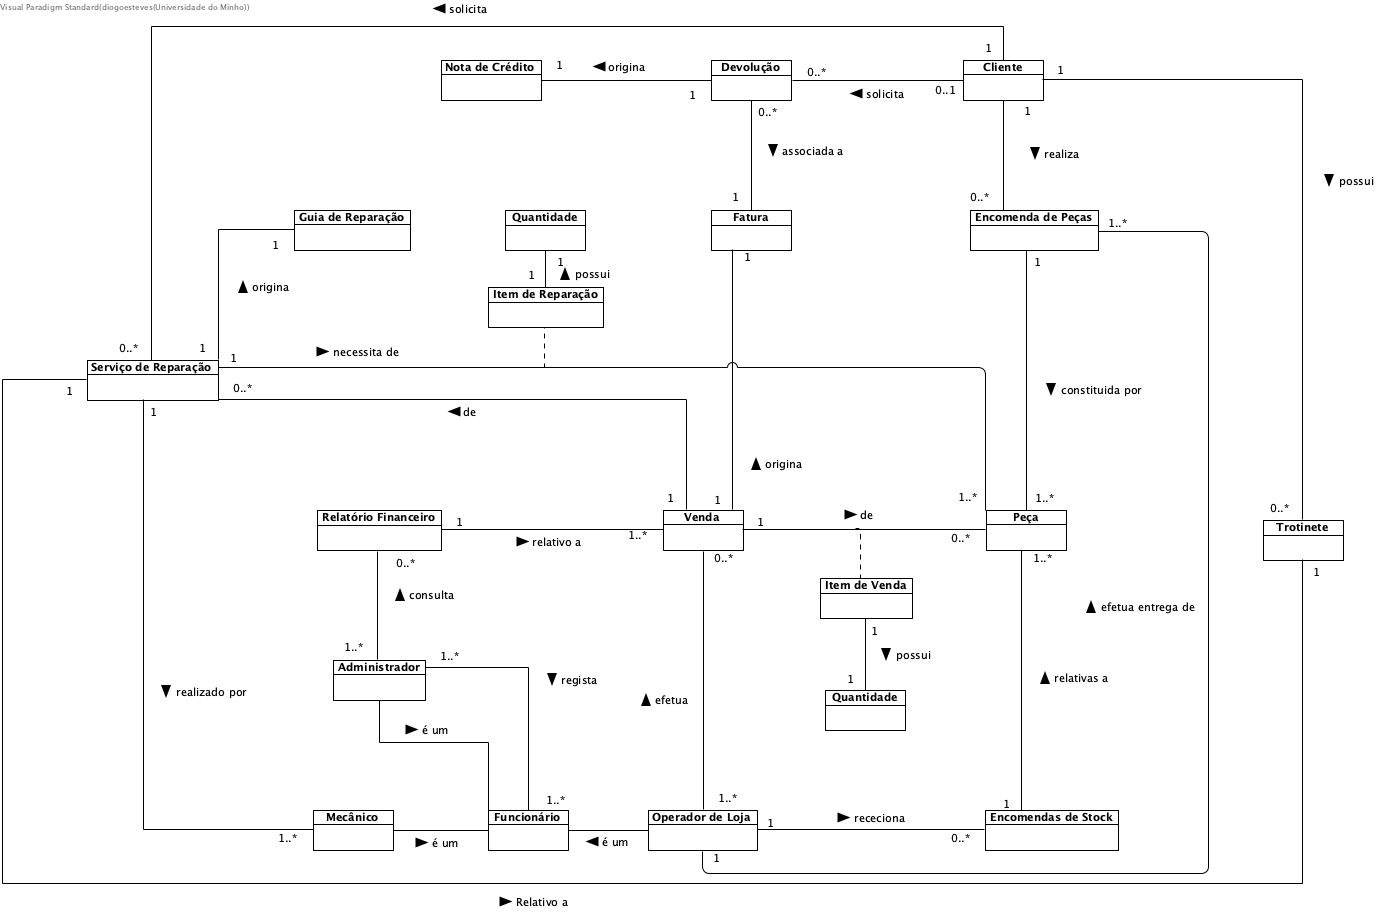
\includegraphics[scale=0.3]{images/Modelo de Domínio.jpg}
        \caption[Modelo de Domínio]{Modelo de Domínio (\hyperref[anexo:modelo_dominio_BIG]{Ver versão ampliada no Anexo})}
        \label{fig:modelo_dominio_pequeno}
    \end{figure}
    
    De forma a sistematizar a interpretação do diagrama, apresentam-se nas subsecções seguintes a descrição das entidades e dos relacionamentos estabelecidos. 
\subsubsection{Dicionário de Entidades}
    A Tabela \ref{tab:entidades_pt1} e a Tabela \ref{tab:entidades_pt2} descrevem as principais classes identificadas no domínio do problema. 
\phantomsection 
    \begin{table}[H]
        \centering
        \renewcommand{\arraystretch}{1.5}
        \begin{tabular}{|p{0.25\textwidth}|p{0.70\textwidth}|}
            \hline
            \rowcolor{gray!20} \textbf{Entidade} & \textbf{Descrição} \\ \hline
            Cliente & Utilizador final detentor das trotinetes e responsável financeiro. \\ \hline
            Trotinete & Veículo sujeito a intervenção técnica e histórico de reparações. \\ \hline
            Serviço de Reparação & Entidade central que agrega diagnóstico, mão-de-obra e peças. \\ \hline
            Venda & Registo de comercialização de peças ou acessórios ao balcão. \\ \hline
            Peça & Artigo físico passível de ser vendido ou incorporado num serviço. \\ \hline
            Fatura & Documento fiscal que formaliza a cobrança de vendas ou serviços. \\ \hline
            Nota de Crédito & Documento retificativo para anulação total ou parcial de faturas. \\ \hline
        \end{tabular}
        \caption{Dicionário de Entidades do Modelo de Domínio (Parte 1)}
        \label{tab:entidades_pt1}
    \end{table}

    \phantomsection 
    \begin{table}[H]
        \centering
        \renewcommand{\arraystretch}{1.5}
        \begin{tabular}{|p{0.25\textwidth}|p{0.70\textwidth}|}
            \hline
            \rowcolor{gray!20} \textbf{Entidade} & \textbf{Descrição} \\ \hline
 
            Devolução & Processo de retorno de artigos ou serviços, originando crédito ao cliente. \\ \hline 
            Encomenda de Peças & Registo de pedido de componentes para aprovisionamento técnico. \\ \hline 
            Guia de Reparação & Documento operacional que orienta o técnico na execução do serviço. \\ \hline 
            Funcionário & Colaborador da empresa com credenciais de acesso ao sistema. \\ \hline 
            Operador de Loja & Especialização de funcionário focada em vendas e receção. \\ \hline
            Mecânico & Especialização de funcionário focada em diagnóstico e reparação. \\ \hline 
            Administrador & Perfil com privilégios elevados para gestão e parametrização. \\ \hline 
        \end{tabular}
        \caption{Dicionário de Entidades do Modelo de Domínio (Parte 2)}
        \label{tab:entidades_pt2}
    \end{table}

    \subsubsection{Descrição de Relacionamentos}
    As tabelas seguintes explicitam as regras de negócio e cardinalidades extraídas do modelo de domínio atualizado. 
\phantomsection 
    \begin{table}[H]
        \centering
        \renewcommand{\arraystretch}{1.5}
        \begin{tabular}{|p{0.32\textwidth}|p{0.63\textwidth}|}
            \hline
            \rowcolor{gray!20} \textbf{Relacionamento} & \textbf{Regra de Negócio / Cardinalidade} \\ \hline
            Cliente \textit{possui} Trotinete & 1:0..*. Um cliente detém múltiplas trotinetes; cada trotinete pertence a apenas um dono. \\ \hline
            Cliente \textit{solicita} Devolução & 0..1:0..*. Devoluções são iniciadas por clientes; um cliente pode ter várias devoluções históricas. \\ \hline
            Cliente \textit{realiza} Encomenda & 1:0..*. Cada encomenda de peças está vinculada a um único cliente. \\ \hline
            Trotinete \textit{tem} Serviço & 1:0..*. Uma trotinete acumula um histórico de intervenções técnicas ao longo do seu ciclo de vida. \\ \hline
            Serviço \textit{origina} Guia & 1:1. Cada ordem de reparação gera obrigatoriamente um documento de guia técnica. \\ \hline
            Serviço \textit{realizado por} Mecânico & 1:1..*. Uma reparação pode exigir a intervenção de um ou mais técnicos mecânicos. \\ \hline
            Serviço \textit{necessita de} Peça & 1:1..*. Intervenções de oficina consomem obrigatoriamente um ou mais componentes de \textit{stock}. \\ \hline
        \end{tabular}
        \caption{Descrição de Relacionamentos do Modelo de Domínio (Parte 1)}
        \label{tab:rel_pt1}
    \end{table}

    \phantomsection 
    \begin{table}[H]
        \centering
        \renewcommand{\arraystretch}{1.5}
        \begin{tabular}{|p{0.32\textwidth}|p{0.63\textwidth}|}
            \hline
            \rowcolor{gray!20} \textbf{Relacionamento} & \textbf{Regra de Negócio / Cardinalidade} \\ \hline
            Venda \textit{origina} Fatura & 1:1. Cada transação comercial gera exatamente um documento fiscal de faturação. \\ \hline
            Devolução \textit{origina} N. Crédito & 1:1. Um processo de devolução concluído resulta na emissão de uma Nota de Crédito. \\ \hline
            Devolução \textit{associa-se} Fatura & 0..*:1. Uma devolução refere-se obrigatoriamente a uma fatura previamente emitida. \\ \hline
            Operador \textit{efetua} Venda & 1..*:0..*. Vendas são processadas por operadores de loja (um ou mais por transação). \\ \hline
            Venda \textit{contém} Peça & 1:1..*. Uma venda pode envolver múltiplos artigos físicos de \textit{stock}. \\ \hline
            Relatório \textit{relativo a} Venda & 1:1..*. Documentos financeiros agregam dados de múltiplas vendas para análise. \\ \hline
            Administrador \textit{consulta} Relatório & 1..*:0..*. Apenas administradores possuem acesso à consulta de relatórios financeiros. \\ \hline
        \end{tabular}
        \caption{Descrição de Relacionamentos do Modelo de Domínio (Parte 2)}
        \label{tab:rel_pt2}
    \end{table}

\pagebreak

\subsection{Levantamento e especificação de Casos de Uso}
\paragraph{}A próxima fase da modelação do problema consiste na identificação e documentação das interações fundamentais entre os diversos atores e o sistema. Para tal, procedeu-se ao levantamento de \textit{Use Cases} (Casos de Uso), uma etapa crucial que permite mapear os requisitos funcionais da plataforma de partilha de trotinetes a partir da perspetiva de quem com ela interage. \paragraph{}Nesta secção, são detalhados os cenários de utilização previstos para os diferentes perfis de utilizador. Estes incluem, tipicamente, o cliente comum (focado no registo, aluguer, pagamento e localização de trotinetes) e o administrador ou equipa de manutenção (responsáveis pela gestão da frota, registo de reparações e monitorização global do sistema). \paragraph{}Através da apresentação dos diagrama de casos de uso e das respetivas descrições textuais, pretende-se clarificar o comportamento esperado do sistema em cada operação, estabelecendo assim a base estrutural necessária para o subsequente desenho da arquitetura e desenvolvimento do software. Os diagramas estão sub-divididos por ator envolvido, no sentido de facilitar a leitura do mesmo. 
\begin{figure}[!h]
        \centering
        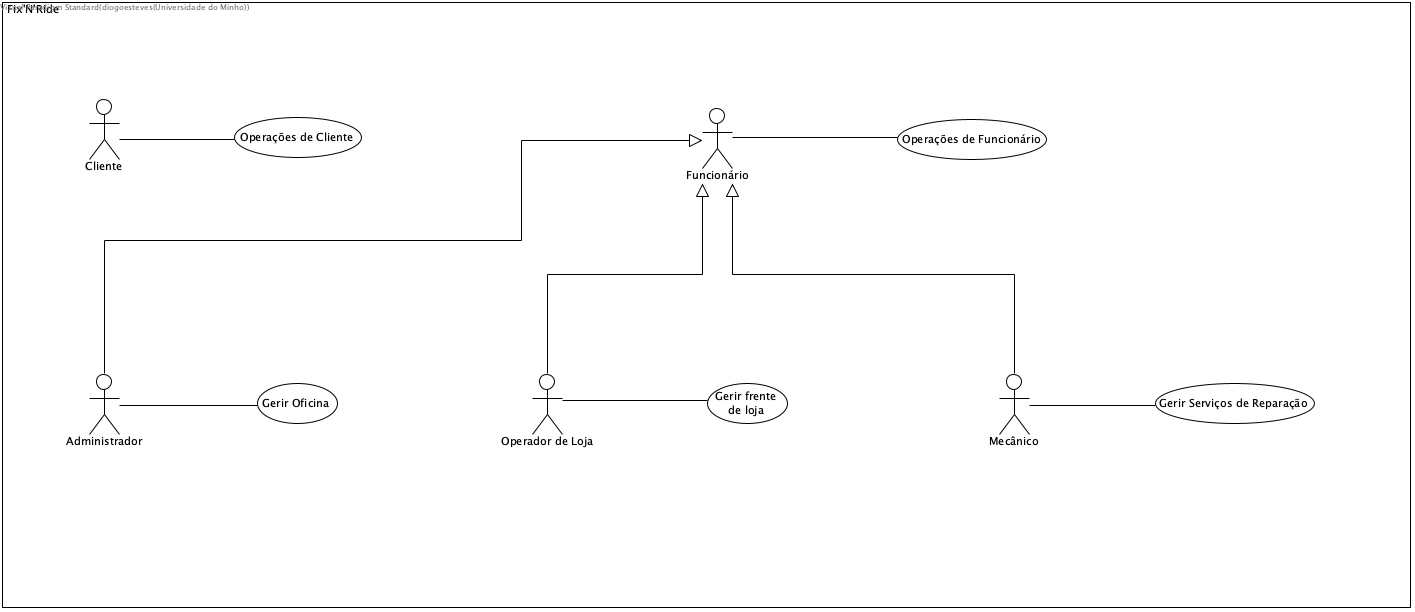
\includegraphics[scale=0.3]{images/Global Use Case.jpg}
        \caption[Diagrama de casos de uso global]{Diagrama de casos de uso global do sistema Fix'n'Ride}
        \label{fig:uc_global}
\end{figure}

\paragraph{}O primeiro diagrama é referente ao diagrama global de casos de uso. Este diagrama ilustra a visão macrouniversal das interações com o sistema \textit{Fix'n'Ride}, separando claramente os fluxos direcionados ao utilizador externo das operações de gestão interna. Um aspeto central deste modelo é a utilização da relação de generalização (herança) para modelar a equipa da oficina: o ator genérico "Funcionário" agrega os comportamentos transversais a todo o \textit{staff} (representados pelas "Operações de Funcionário", como a autenticação no sistema). Este ator é depois especializado em três perfis de acesso distintos, consoante as suas competências práticas: o "Administrador", responsável por "Gerir Oficina"\space (relatórios, promoções e aprovações); o "Operador de Loja", focado em "Gerir frente de loja"\space (receção, vendas diretas e entregas); e o "Mecânico", encarregue de "Gerir Serviços de Reparação" (triagem técnica e execução de intervenções).Em paralelo, o "Cliente"\space atua como um ator independente, interagindo exclusivamente com o pacote de "Operações de Cliente", o qual engloba ações como o agendamento de diagnósticos e a consulta de histórico. 
\begin{figure}[!h]
        \centering
        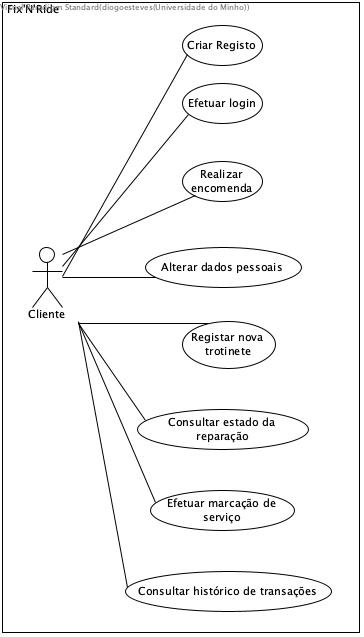
\includegraphics[scale=0.4]{images/Cliente Use Case.jpg}
        \caption[Diagrama de casos de uso das operações do cliente]{Diagrama de casos de uso das operações do cliente no sistema Fix'n'Ride}
        \label{fig:uc_cliente}
\end{figure}

\paragraph{}O segundo diagrama foca-se especificamente no pacote de "Operações de Cliente", detalhando as interações que o utilizador final pode realizar na sua área reservada do sistema Fix'n'Ride. O ator principal, o "Cliente", possui autonomia para gerir o seu perfil através dos casos de uso "Criar Registo", "Efetuar login"\space e "Alterar dados pessoais". No que diz respeito à componente comercial, o cliente tem a capacidade de "Realizar encomenda"\space de peças diretamente pelo catálogo online e "Consultar histórico de transações", permitindo-lhe gerir as suas faturas passadas. Relativamente à assistência técnica, o diagrama evidencia o fluxo de "Registar nova trotinete"\space para associar veículos ao seu perfil, "Efetuar marcação de serviço"\space para agendar diagnósticos e "Consultar estado da reparação", garantindo que o utilizador acompanha o progresso das intervenções em tempo real sem necessitar de contactar a oficina. 
\begin{figure}[!h]
    \centering
    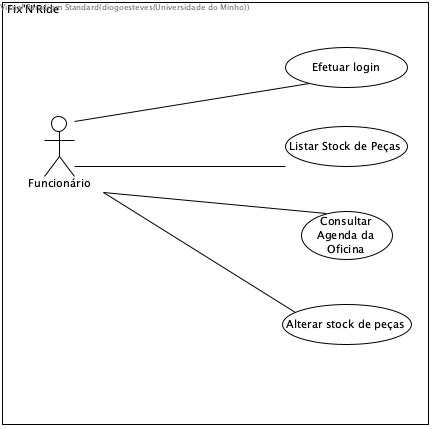
\includegraphics[scale=0.4]{images/Funcionário Use Case.jpg}
    \caption[Diagrama de casos de uso das operações do funcionário]{Diagrama de casos de uso das operações do funcionário no sistema Fix'n'Ride}
    \label{fig:uc_funcionario}
\end{figure}

\paragraph{}O terceiro diagrama foca-se no ator genérico "Funcionário"\space. Este perfil encapsula as operações de base partilhadas por todos os membros do \textit{staff} da oficina, independentemente da sua especialização. As ações incluem a autenticação na plataforma através do caso de uso "Efetuar login", a verificação rápida de inventário com o "Listar Stock de Peças"\space e o ajuste de discrepâncias com o "Alterar stock de peças"\space. Adicionalmente, este ator tem acesso transversal à organização do trabalho através do caso de uso "Consultar Agenda da Oficina", permitindo a qualquer colaborador visualizar as reparações e entregas planeadas para o dia. 
\clearpage

\begin{figure}[!h]
    \centering
    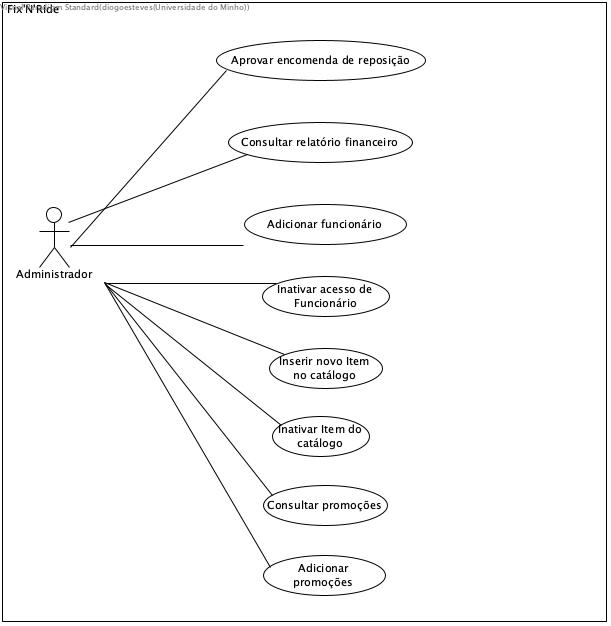
\includegraphics[scale=0.4]{images/Administrador Use Case.jpg}
    \caption[Diagrama de casos de uso das operações do administrador]{Diagrama de casos de uso das operações do administrador no sistema Fix'n'Ride}
    \label{fig:uc_administrador}
\end{figure}

\paragraph{}O quarto diagrama detalha as interações do "Administrador", o perfil com os privilégios mais elevados no sistema. Este ator é responsável pela gestão e parametrização do negócio. No âmbito financeiro e de \textit{stock}, o administrador interage com os casos de uso "Aprovar encomenda de reposição"\space e "Consultar relatório financeiro"\space. Na vertente comercial, gere os preços e as tabelas através dos fluxos "Inserir novo Item no catálogo", "Inativar Item do catálogo", "Consultar promoções"\space e "Adicionar promoções"\space. Por fim, assegura o controlo de acessos e a organização da equipa através dos casos de uso "Adicionar funcionário"\space e "Inativar acesso de Funcionário"\space. 
\clearpage

\begin{figure}[!h]
    \centering
    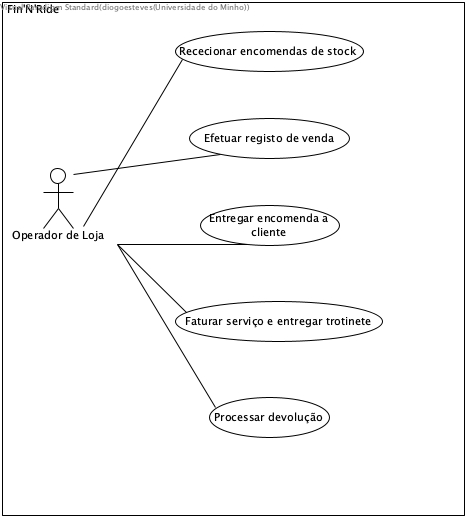
\includegraphics[scale=0.4]{images/Operador de Loja Use Case.jpg}
    \caption[Diagrama de casos de uso das operações do operador de loja]{Diagrama de casos de uso das operações do operador de loja no sistema Fix'n'Ride}
    \label{fig:uc_operador}
\end{figure}

\paragraph{}O quinto diagrama ilustra as responsabilidades do "Operador de Loja", que atua na linha da frente comercial e no controlo de entradas físicas de material. As suas interações refletem o atendimento direto ao balcão e a logística diária. Este ator é responsável por "Rececionar encomendas de stock"\space provenientes dos fornecedores. No atendimento ao público, conduz transações rápidas através de "Efetuar registo de venda"\space e "Entregar encomenda a cliente"\space. Além disso, é o responsável por finalizar os processos da oficina perante o cliente, utilizando os casos de uso "Faturar serviço e entregar trotinete"\space e, caso seja necessário, "Processar devolução"\space. 
\clearpage

\begin{figure}[!h]
    \centering
    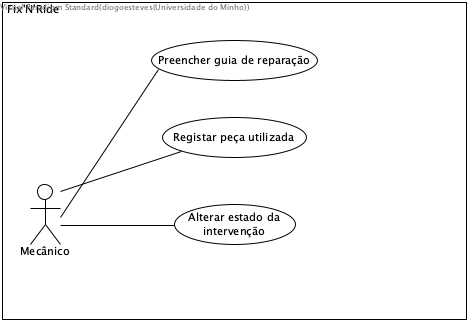
\includegraphics[scale=0.4]{images/Mecânico Use Case.jpg}
    \caption[Diagrama de casos de uso das operações do mecânico]{Diagrama de casos de uso das operações do mecânico no sistema Fix'n'Ride}
    \label{fig:uc_mecanico}
\end{figure}

\paragraph{}O sexto e último diagrama de casos de uso está centrado no "Mecânico", o ator responsável pela execução técnica e intervenção direta nas trotinetes. As suas operações estão desenhadas para serem realizadas a partir da bancada de trabalho, minimizando a carga administrativa. O fluxo inicia-se com a triagem do veículo, onde o mecânico interage com o sistema para "Preencher guia de reparação"\space. Durante a execução do serviço, este utiliza o caso de uso "Registar peça utilizada"\space para garantir a rastreabilidade dos componentes instalados e deduzi-los do inventário. Ao longo de todo o processo, o ator gere o progresso do trabalho através do caso de uso "Alterar estado da intervenção", garantindo que o cliente e o restante \textit{staff} se mantêm atualizados sobre a reparação. 
\subsubsection{Especificação Detalhada dos Casos de Uso}

Nesta secção, apresenta-se a descrição detalhada dos principais Casos de Uso (Use Cases) do sistema, focando no fluxo interativo entre os diferentes atores e a aplicação para satisfazer os requisitos operacionais da MobiFix. 
% ---------------- USE CASE 1 ----------------
\begin{longtable}{|>{\columncolor{black!10}\bfseries}p{3.5cm}|p{11.5cm}|}
\hline
Use Case & \textbf{UC01 -- Efetuar marcação de serviço} \\ \hline
\endfirsthead

\multicolumn{2}{c}%
{{\bfseries Continuação da Tabela \thetable{} — UC01 -- Efetuar marcação de serviço}} \\
\hline
Use Case & \textbf{UC01 -- Efetuar marcação de serviço} \\ \hline
\endhead

\hline \multicolumn{2}{r}{{\textit{Continua na próxima página}}} \\ \hline
\endfoot

\hline
\caption{Descrição detalhada do caso de uso — Efetuar marcação de serviço.}
\label{tab:uc1}
\endlastfoot

% --- CONTEÚDO DA TABELA ---

Cenários & 
\begin{itemize}[leftmargin=*, nosep, topsep=2pt, partopsep=0pt]
    \item O Cliente faz a marcação de um serviço de reparação para a sua trotinete.
\end{itemize} \\ \hline

Descrição & O cliente escolhe um horário disponível na agenda da oficina para entregar a sua trotinete para diagnóstico e posterior reparação. \\ \hline

Pré-condições & 
\begin{itemize}[leftmargin=*, nosep, topsep=2pt, partopsep=0pt]
    \item O Cliente tem sessão iniciada no sistema.
    \item O Cliente tem, pelo menos, uma trotinete registada no seu perfil.
\end{itemize} \\ \hline

Pós-condições & 
\begin{itemize}[leftmargin=*, nosep, topsep=2pt, partopsep=0pt]
    \item O serviço de diagnóstico é registado na agenda da oficina com o estado "Agendado".
    \item O horário selecionado fica indisponível para outros clientes.
\end{itemize} \\ \hline

Fluxo normal & 
\begin{enumerate}[leftmargin=*, nosep, topsep=2pt, partopsep=0pt]
    \item O cliente acede à sua área reservada e seleciona a opção de "realizar marcação de diagnóstico".
    \item O sistema lista as trotinetes associadas ao cliente.
    \item O cliente seleciona a trotinete a intervencionar.
    \item O sistema informa o cliente que o preço final depende do diagnóstico presencial do técnico.
    \item O sistema apresenta as \textit{slots} de horário disponíveis na oficina.
    \item O cliente seleciona o dia e a hora desejados.
    \item O sistema regista o diagnóstico na agenda da oficina.
\end{enumerate} \\ \hline

\end{longtable}

% ---------------- USE CASE 2 ----------------
\begin{longtable}{|>{\columncolor{black!10}\bfseries}p{3.5cm}|p{11.5cm}|}
\hline
Use Case & \textbf{UC02 -- Preencher guia de reparação} \\ \hline
\endfirsthead

\multicolumn{2}{c}%
{{\bfseries Continuação da Tabela \thetable{} — UC02 -- Preencher guia de reparação}} \\
\hline
Use Case & \textbf{UC02 -- Preencher guia de reparação} \\ \hline
\endhead

\hline \multicolumn{2}{r}{{\textit{Continua na próxima página}}} \\ \hline
\endfoot

\hline
\caption{Descrição detalhada do caso de uso — Preencher guia de reparação.}
\label{tab:uc2}
\endlastfoot


Cenários & 
\begin{itemize}[leftmargin=*, nosep, topsep=2pt, partopsep=0pt]
    \item Um mecânico realiza o diagnóstico de um serviço de reparação agendado, e o sistema faz a marcação no horário dos mecânicos.
\end{itemize} \\ \hline

Descrição & Um mecânico de triagem preenche a guia de reparação referente a um pedido submetido pelo cliente, inserindo o respetivo diagnóstico. Subsequentemente, o sistema processa esses dados e efetua a alocação automática da reparação para o horário de atendimento de um mecânico com a especialidade requerida. \\ \hline

Pré-condições & 
\begin{itemize}[leftmargin=*, nosep, topsep=2pt, partopsep=0pt]
    \item O mecânico de triagem iniciou sessão no sistema.
    \item O cliente apresentou-se em loja, junto da trotinete a ser reparada.
\end{itemize} \\ \hline

Pós-condições & 
\begin{itemize}[leftmargin=*, nosep, topsep=2pt, partopsep=0pt]
    \item É efetuada uma marcação para o horário de atendimento de um mecânico com a especialidade necessária para a reparação.
    \item É gerada uma guia de reparação com o diagnóstico do mecânico, com o tipo do serviço a ser executado, com o \textit{feedback do cliente}, e com os dados de faturação do cliente.
\end{itemize} \\ \hline

Fluxo normal & 
\begin{enumerate}[leftmargin=*, nosep, topsep=2pt, partopsep=0pt]
    \item O mecânico de triagem seleciona na agenda da oficina o serviço agendado pelo cliente.
    \item O sistema apresenta os dados do cliente, bem como a trotinete associada à marcação.
    \item Após realizar o diagnóstico da trotinete, o mecânico de triagem seleciona a opção de "gerar guia de reparação".
    \item O sistema apresenta um formulário, de preenchimento obrigatório, com os dados do cliente pré-preenchidos, e com a área de inserção de descrição do diagnóstico e \textit{feedback} do cliente, bem como de seleção de tipo(s) de intervenções a executar.
    \item O mecânico de triagem preenche a descrição do diagnóstico e do \textit{feedback} e seleciona as intervenções necessárias.
    \item O sistema apresenta uma pré-visualização da guia de diagnóstico.
    \item O mecânico de triagem confirma os dados da guia com o cliente.
    \item O sistema realiza a marcação de reparação na agenda do(s) técnico(s) especializado(s) nas intervenções identificadas na triagem.
    \item O sistema envia por email a guia de reparação ao cliente, com os dados do formulário.
\end{enumerate} \\ \hline

Fluxo de Exceção 1 & [Cliente não concorda com os termos da guia] (passo 7):
\begin{enumerate}[label=7.\arabic*., leftmargin=*, nosep, topsep=2pt, partopsep=0pt]
    \item O cliente não concorda com os termos da guia de reparação.
    \item O processo de agendamento do serviço é cancelado.
\end{enumerate} \\ \hline

\end{longtable}

% ---------------- USE CASE 3 ----------------
% ---------------- USE CASE 3 ----------------
\begin{longtable}{|>{\columncolor{black!10}\bfseries}p{3.5cm}|p{11.5cm}|}
\hline
Use Case & \textbf{UC03 -- Realizar Venda Direta ao Balcão} \\ \hline
\endfirsthead

\multicolumn{2}{c}%
{{\bfseries Continuação da Tabela \thetable{} — UC03 -- Realizar Venda Direta ao Balcão}} \\
\hline
Use Case & \textbf{UC03 -- Realizar Venda Direta ao Balcão} \\ \hline
\endhead

\hline \multicolumn{2}{r}{{\textit{Continua na próxima página}}} \\ \hline
\endfoot

\hline
\caption{Descrição detalhada do caso de uso — Realizar Venda Direta ao Balcão}
\label{tab:uc3}
\endlastfoot

Cenários & 
\begin{itemize}[leftmargin=*, nosep, topsep=2pt, partopsep=0pt]
    \item O Operador de Loja efetua a venda de uma peça diretamente a um cliente.
\end{itemize} \\ \hline

Descrição & O cliente adquire uma peça em loja sem necessitar de intervenção técnica por parte dos mecânicos, procedendo ao pagamento imediato. \\ \hline

Pré-condições & 
\begin{itemize}[leftmargin=*, nosep, topsep=2pt, partopsep=0pt]
    \item O sistema está operacional.
    \item O Operador de Loja iniciou sessão no sistema.
    \item O artigo solicitado existe no catálogo do sistema.
\end{itemize} \\ \hline

Pós-condições & 
\begin{itemize}[leftmargin=*, nosep, topsep=2pt, partopsep=0pt]
    \item O \textit{stock} físico da peça vendida é decrementado.
    \item A fatura da venda é emitida no sistema.
    \item O valor financeiro é adicionado ao relatório do dia.
\end{itemize} \\ \hline

Fluxo normal & 
\begin{enumerate}[leftmargin=*, nosep, topsep=2pt, partopsep=0pt]
    \item O Operador de Loja pesquisa e seleciona a peça solicitada no catálogo.
    \item O Operador adiciona o artigo à funcionalidade de Venda Direta.
    \item O sistema apresenta o valor a pagar.
    \item O Operador confirma o recebimento do pagamento.
    \item O sistema emite a fatura.
    \item O sistema baixa uma unidade ao \textit{stock} do inventário.
    \item O sistema regista o lucro na operação financeira.
\end{enumerate} \\ \hline

Fluxo alternativo 1 & [Geração de encomenda automática] (passo 6):
\begin{enumerate}[label=6.\arabic*, leftmargin=*, nosep, topsep=2pt, partopsep=0pt]
    \item O sistema verifica que a venda fez o \textit{stock} atingir o nível mínimo configurado.
    \item O sistema sugere/cria uma Encomenda de Reposição pendente para a Administração.
    \item O fluxo prossegue normalmente para o passo 7.
\end{enumerate} \\ \hline

\end{longtable}
% ---------------- USE CASE 4 ----------------
\begin{longtable}{|>{\columncolor{black!10}\bfseries}p{3.5cm}|p{11.5cm}|}
\hline
Use Case & \textbf{UC04 -- Aprovar Encomenda de Reposição} \\ \hline
\endfirsthead

\multicolumn{2}{c}%
{{\bfseries Continuação da Tabela \thetable{} — UC04 -- Aprovar Encomenda de Reposição}} \\
\hline
Use Case & \textbf{UC04 -- Aprovar Encomenda de Reposição} \\ \hline
\endhead

\hline \multicolumn{2}{r}{{\textit{Continua na próxima página}}} \\ \hline
\endfoot

\hline
\caption{Descrição detalhada do caso de uso — Aprovar Encomenda de Reposição}
\label{tab:uc4}
\endlastfoot

Cenários & 
\begin{itemize}[leftmargin=*, nosep, topsep=2pt, partopsep=0pt]
    \item O Administrador analisa e aprova uma ordem de reposição de \textit{stock} gerada pelo sistema.
\end{itemize} \\ \hline

Descrição & O sistema alerta para a necessidade de repor \textit{stock} de uma peça. O administrador revê a nota de encomenda pendente, ajusta as quantidades se necessário e aprova a compra. \\ \hline

Pré-condições & 
\begin{itemize}[leftmargin=*, nosep, topsep=2pt, partopsep=0pt]
    \item O sistema está operacional.
    \item O utilizador com perfil de Administrador iniciou sessão.
    \item O \textit{stock} de pelo menos uma peça atingiu o limite mínimo, gerando uma pendência.
\end{itemize} \\ \hline

Pós-condições & 
\begin{itemize}[leftmargin=*, nosep, topsep=2pt, partopsep=0pt]
    \item O estado da encomenda passa a "Em Trânsito".
\end{itemize} \\ \hline

Fluxo normal & 
\begin{enumerate}[leftmargin=*, nosep, topsep=2pt, partopsep=0pt]
    \item O administrador acede ao menu de gestão de encomendas.
    \item O sistema lista as encomendas com estado "Pendente".
    \item O administrador seleciona a encomenda pendente a rever.
    \item O sistema exibe os detalhes (peça, fornecedor, quantidade sugerida, custo estimado).
    \item O administrador verifica a informação e clica em "Aprovar".
    \item O sistema atualiza o registo para "Em Trânsito".
\end{enumerate} \\ \hline

Fluxo alternativo 1 & [Ajuste de quantidade] (passo 4):
\begin{enumerate}[label=4.\arabic*., leftmargin=*, nosep, topsep=2pt, partopsep=0pt]
    \item O administrador decide encomendar uma quantidade diferente da sugerida.
    \item O administrador altera o valor no campo de quantidade.
    \item O sistema recalcula instantaneamente o custo estimado.
    \item O fluxo regressa ao passo 5.
\end{enumerate} \\ \hline

Fluxo de exceção 1 & [Rejeitar Encomenda] (passo 5):
\begin{enumerate}[label=5.\arabic*., leftmargin=*, nosep, topsep=2pt, partopsep=0pt]
    \item O administrador decide não avançar com a compra e seleciona "Rejeitar/Cancelar".
    \item O sistema cancela a encomenda pendente e remove-a da lista.
    \item O fluxo termina.
\end{enumerate} \\ \hline

\end{longtable}
% ---------------- USE CASE 5 ----------------
% ---------------- USE CASE 5 ----------------
\begin{longtable}{|>{\columncolor{black!10}\bfseries}p{3.5cm}|p{11.5cm}|}
\hline
Use Case & \textbf{UC05 -- Faturar Serviço e Entregar Trotinete} \\ \hline
\endfirsthead

\multicolumn{2}{c}%
{{\bfseries Continuação da Tabela \thetable{} — UC05 -- Faturar Serviço e Entregar Trotinete}} \\
\hline
Use Case & \textbf{UC05 -- Faturar Serviço e Entregar Trotinete} \\ \hline
\endhead

\hline \multicolumn{2}{r}{{\textit{Continua na próxima página}}} \\ \hline
\endfoot

\hline
\caption{Descrição detalhada do caso de uso — Faturar Serviço e Entregar Trotinete}
\label{tab:uc5}
\endlastfoot

Cenários & 
\begin{itemize}[leftmargin=*, nosep, topsep=2pt, partopsep=0pt]
    \item O Operador de Loja recebe o cliente, emite a fatura e entrega a trotinete reparada.
\end{itemize} \\ \hline

Descrição & Conclusão do ciclo de reparação, onde o serviço dado como "Pronto"\space pelo mecânico é pago pelo cliente e faturado. \\ \hline

Pré-condições & 
\begin{itemize}[leftmargin=*, nosep, topsep=2pt, partopsep=0pt]
    \item O sistema está operacional.
    \item O Operador de Loja iniciou sessão.
    \item A Ordem de Serviço (OS) correspondente encontra-se no estado "Concluido".
\end{itemize} \\ \hline

Pós-condições & 
\begin{itemize}[leftmargin=*, nosep, topsep=2pt, partopsep=0pt]
    \item A Ordem de Serviço transita para "Fechado".
    \item O documento fiscal (fatura única) é gerado no sistema e enviado para o cliente.
\end{itemize} \\ \hline

Fluxo normal & 
\begin{enumerate}[leftmargin=*, nosep, topsep=2pt, partopsep=0pt]
    \item O cliente apresenta-se na receção para levantar o equipamento.
    \item O Operador pesquisa pela OS associada ao cliente.
    \item O sistema apresenta os detalhes do serviço concluído e o valor final (peças e mão de obra).
    \item O Operador seleciona a via de pagamento e confirma a transação.
    \item O sistema emite a fatura única para o cliente.
    \item O Operador entrega a trotinete fisicamente.
    \item O sistema altera o estado da OS para "Fechado"\space e arquiva-a, enviando também a fatura para o \textit{email} do cliente.
\end{enumerate} \\ \hline

Fluxo de exceção 1 & [Falha no pagamento] (passo 4):
\begin{enumerate}[label=4.\arabic*., leftmargin=*, nosep, topsep=2pt, partopsep=0pt]
    \item O pagamento (ex: cartão ou \textit{MBWay}) é rejeitado.
    \item O Operador cancela a operação no sistema.
    \item O sistema mantém a OS no estado "Concluido".
    \item A entrega da trotinete é suspensa.
\end{enumerate} \\ \hline

\end{longtable}

% ---------------- USE CASE 6 ----------------
% ---------------- USE CASE 6 ----------------
\begin{longtable}{|>{\columncolor{black!10}\bfseries}p{3.5cm}|p{11.5cm}|}
\hline
Use Case & \textbf{UC06 -- Consultar Relatórios Operacionais} \\ \hline
\endfirsthead

\multicolumn{2}{c}%
{{\bfseries Continuação da Tabela \thetable{} — UC06 -- Consultar Relatórios Operacionais}} \\
\hline
Use Case & \textbf{UC06 -- Consultar Relatórios Operacionais} \\ \hline
\endhead

\hline \multicolumn{2}{r}{{\textit{Continua na próxima página}}} \\ \hline
\endfoot

\hline
\caption{Descrição detalhada do caso de uso — Consultar Relatórios Operacionais}
\label{tab:uc6}
\endlastfoot

Cenários & 
\begin{itemize}[leftmargin=*, nosep, topsep=2pt, partopsep=0pt]
    \item O Administrador acede aos \textit{dashboards} para analisar a performance da oficina e métricas de faturação.
\end{itemize} \\ \hline

Descrição & Geração de relatórios com indicadores de desempenho (KPIs), como tempo médio de reparação, faturação e peças mais consumidas. \\ \hline

Pré-condições & 
\begin{itemize}[leftmargin=*, nosep, topsep=2pt, partopsep=0pt]
    \item O sistema está operacional e contém dados históricos registados.
    \item O utilizador com perfil de Administrador iniciou sessão.
\end{itemize} \\ \hline

Pós-condições & 
\begin{itemize}[leftmargin=*, nosep, topsep=2pt, partopsep=0pt]
    \item Nenhuma (operação exclusiva de leitura/consulta).
\end{itemize} \\ \hline

Fluxo normal & 
\begin{enumerate}[leftmargin=*, nosep, topsep=2pt, partopsep=0pt]
    \item O administrador navega até ao módulo de Reporting.
    \item O administrador seleciona o intervalo de datas pretendido (ex: Último Mês).
    \item O administrador clica no botão "Gerar Relatório".
    \item O sistema processa os dados da base de dados (Vendas, Serviços e peças).
    \item O sistema apresenta o \textit{dashboard} com gráficos e totais agregados.
\end{enumerate} \\ \hline

Fluxo alternativo 1 & [Exportar Documento] (passo 5):
\begin{enumerate}[label=5.\arabic*., leftmargin=*, nosep, topsep=2pt, partopsep=0pt]
    \item O administrador clica em "Exportar Relatório".
    \item O sistema compila os dados visíveis e inicia o \textit{download} de um ficheiro PDF.
    \item O fluxo termina.
\end{enumerate} \\ \hline

\end{longtable}

% ---------------- USE CASE 7 ----------------
% ---------------- USE CASE 7 ----------------
\begin{longtable}{|>{\columncolor{black!10}\bfseries}p{3.5cm}|p{11.5cm}|}
\hline
Use Case & \textbf{UC07 -- Inserir Novo Item no Catálogo} \\ \hline
\endfirsthead

\multicolumn{2}{c}%
{{\bfseries Continuação da Tabela \thetable{} — UC07 -- Inserir Novo Item no Catálogo}} \\
\hline
Use Case & \textbf{UC07 -- Inserir Novo Item no Catálogo} \\ \hline
\endhead

\hline \multicolumn{2}{r}{{\textit{Continua na próxima página}}} \\ \hline
\endfoot

\hline
\caption{Descrição detalhada do caso de uso — Inserir Novo Item no Catálogo}
\label{tab:uc7}
\endlastfoot

Cenários & 
\begin{itemize}[leftmargin=*, nosep, topsep=2pt, partopsep=0pt]
    \item O Administrador regista uma nova peça para passar a estar disponível na oficina.
\end{itemize} \\ \hline

Descrição & Adição de um novo registo (peça ou serviço) ao catálogo central do sistema, estipulando os seus custos e preço de venda. \\ \hline

Pré-condições & 
\begin{itemize}[leftmargin=*, nosep, topsep=2pt, partopsep=0pt]
    \item O sistema está operacional.
    \item O utilizador com perfil de Administrador iniciou sessão.
\end{itemize} \\ \hline

Pós-condições & 
\begin{itemize}[leftmargin=*, nosep, topsep=2pt, partopsep=0pt]
    \item O novo item é gravado na base de dados e passa a estar imediatamente disponível para venda e orçamentação.
\end{itemize} \\ \hline

Fluxo normal & 
\begin{enumerate}[leftmargin=*, nosep, topsep=2pt, partopsep=0pt]
    \item O administrador acede ao menu de gestão de Catálogo de Peças e Serviços.
    \item O administrador seleciona a opção "Novo Registo".
    \item O sistema apresenta o formulário de inserção.
    \item O administrador preenche os dados (Categoria, Referência, Descrição, Fornecedor, Custos e PVP).
    \item O administrador clica em "Guardar".
    \item O sistema valida a formatação dos dados e grava a nova entidade.
    \item O sistema atualiza e exibe a grelha do catálogo com a nova entrada.
\end{enumerate} \\ \hline

Fluxo de exceção 1 & [Referência Duplicada] (passo 6):
\begin{enumerate}[label=6.\arabic*., leftmargin=*, nosep, topsep=2pt, partopsep=0pt]
    \item O sistema deteta que a Referência/Código EAN introduzido já existe na base de dados.
    \item O sistema interrompe a gravação e exibe uma notificação de erro ao administrador.
    \item O fluxo regressa ao passo 4 para correção do campo.
\end{enumerate} \\ \hline

\end{longtable}

% ---------------- USE CASE 8 ----------------

\begin{longtable}{|>{\columncolor{black!10}\bfseries}p{3.5cm}|p{11.5cm}|}
\hline
Use Case & \textbf{UC08 -- Registar Conta de Cliente} \\ \hline
\endfirsthead

\multicolumn{2}{c}%
{{\bfseries Continuação da Tabela \thetable{} — UC08 -- Registar Conta de Cliente}} \\
\hline
Use Case & \textbf{UC08 -- Registar Conta de Cliente} \\ \hline
\endhead

\hline \multicolumn{2}{r}{{\textit{Continua na próxima página}}} \\ \hline
\endfoot

\hline
\caption{Descrição detalhada do caso de uso — Registar Conta de Cliente.}
\label{tab:uc8}
\endlastfoot

% --- CONTEÚDO DA TABELA ---

Cenários & 
\begin{itemize}[leftmargin=*, nosep, topsep=2pt, partopsep=0pt]
    \item Um novo utilizador cria uma conta no sistema para poder agendar serviços e comprar peças online.
\end{itemize} \\ \hline

Descrição & O utilizador fornece os seus dados pessoais e de faturação para criar um perfil de acesso ao portal do cliente. \\ \hline

Pré-condições & 
\begin{itemize}[leftmargin=*, nosep, topsep=2pt, partopsep=0pt]
    \item O sistema está operacional.
\end{itemize} \\ \hline

Pós-condições & 
\begin{itemize}[leftmargin=*, nosep, topsep=2pt, partopsep=0pt]
    \item É criado um novo registo na tabela de Clientes.
    \item O cliente fica apto a efetuar \textit{login} na plataforma.
\end{itemize} \\ \hline

Fluxo normal & 
\begin{enumerate}[leftmargin=*, nosep, topsep=2pt, partopsep=0pt]
    \item O utilizador acede à página de criação de conta.
    \item O utilizador preenche os dados solicitados (Nome, Email, Contacto, Morada, NIF e Password).
    \item O utilizador confirma a \textit{password}, repetindo a mesma, e submete o formulário.
    \item O sistema valida os dados e aplica \textit{hashing} à \textit{password}.
    \item O sistema guarda o registo e apresenta uma mensagem de sucesso.
    \item O sistema redireciona o utilizador para a página de \textit{login}.
\end{enumerate} \\ \hline

Fluxo alternativo 1 & [Email já registado] (passo 4):
\begin{enumerate}[label=4.\arabic*., leftmargin=*, nosep, topsep=2pt, partopsep=0pt]
    \item O sistema deteta que o email introduzido já existe na base de dados.
    \item O sistema impede a criação da conta e exibe uma mensagem de erro ("Email já em uso").
    \item O fluxo regressa ao passo 2 para o utilizador corrigir o email ou fazer \textit{login}.
\end{enumerate} \\ \hline

Fluxo alternativo 2 & [\textit{Passwords} não coincidem] (passo 3):
\begin{enumerate}[label=3.\arabic*., leftmargin=*, nosep, topsep=2pt, partopsep=0pt]
    \item O sistema deteta que as \textit{passwords} introduzidas não coincidem e informa o cliente de tal.
    \item O sistema solicita a reinserção da \textit{password}.
    \item O fluxo regressa ao passo 3.
\end{enumerate} \\ \hline

\end{longtable}

% ---------------- USE CASE 9 ----------------
% ---------------- USE CASE 9 ----------------
\begin{longtable}{|>{\columncolor{black!10}\bfseries}p{3.5cm}|p{11.5cm}|}
\hline
Use Case & \textbf{UC09 -- Realizar encomenda} \\ \hline
\endfirsthead

\multicolumn{2}{c}%
{{\bfseries Continuação da Tabela \thetable{} — UC09 -- Realizar encomenda}} \\
\hline
Use Case & \textbf{UC09 -- Realizar encomenda} \\ \hline
\endhead

\hline \multicolumn{2}{r}{{\textit{Continua na próxima página}}} \\ \hline
\endfoot

\hline
\caption{Descrição detalhada do caso de uso — Realizar encomenda.}
\label{tab:uc9}
\endlastfoot

% --- CONTEÚDO DA TABELA ---

Cenários & 
\begin{itemize}[leftmargin=*, nosep, topsep=2pt, partopsep=0pt]
    \item O Cliente adquire peças autonomamente através do catálogo online da loja.
\end{itemize} \\ \hline

Descrição & Fluxo comercial onde o cliente seleciona peças, efetua o pagamento digitalmente e recebe a fatura, para posterior levantamento físico. \\ \hline

Pré-condições & 
\begin{itemize}[leftmargin=*, nosep, topsep=2pt, partopsep=0pt]
    \item O sistema está operacional.
    \item O Cliente iniciou sessão na sua conta.
    \item Existe \textit{stock} das peças desejadas para a realização da encomenda.
\end{itemize} \\ \hline

Pós-condições & 
\begin{itemize}[leftmargin=*, nosep, topsep=2pt, partopsep=0pt]
    \item O \textit{stock} das peças adquiridas é decrementado.
    \item A fatura é gerada e associada ao histórico do cliente.
\end{itemize} \\ \hline

Fluxo normal & 
\begin{enumerate}[leftmargin=*, nosep, topsep=2pt, partopsep=0pt]
    \item O cliente acede ao catálogo na \textit{landing page} e pesquisa peças.
    \item O cliente adiciona as peças desejadas ao carrinho.
    \item O cliente avança para a página de pagamento e revê a encomenda.
    \item O cliente seleciona o método de pagamento (ex: \textit{MBWay}) e efetua o pagamento.
    \item O sistema valida a transação com sucesso.
    \item O sistema emite a fatura e envia o comprovativo de levantamento para o cliente.
    \item O sistema deduz as quantidades no inventário geral.
\end{enumerate} \\ \hline

Fluxo de exceção 1 & [Pagamento Recusado] (passo 5):
\begin{enumerate}[label=5.\arabic*., leftmargin=*, nosep, topsep=2pt, partopsep=0pt]
    \item A entidade bancária recusa o pagamento ou expira o tempo limite.
    \item O sistema informa o cliente da falha na transação.
    \item A encomenda não é registada e o \textit{stock} não é alterado.
    \item O fluxo termina.
\end{enumerate} \\ \hline

Fluxo alternativo 2 & [Atingido \textit{stock} mínimo de peça] (passo 7):
\begin{enumerate}[label=7.\arabic*., leftmargin=*, nosep, topsep=2pt, partopsep=0pt]
    \item O sistema verifica que foi atingido o \textit{stock} mínimo de uma peça envolvida na transação.
    \item O sistema cria uma encomenda de novo \textit{stock} para aprovação da administração.
\end{enumerate} \\ \hline

\end{longtable}

% ---------------- USE CASE 10 ----------------
% ---------------- USE CASE 10 ----------------
\begin{longtable}{|>{\columncolor{black!10}\bfseries}p{3.5cm}|p{11.5cm}|}
\hline
Use Case & \textbf{UC10 -- Adicionar Promoções} \\ \hline
\endfirsthead

\multicolumn{2}{c}%
{{\bfseries Continuação da Tabela \thetable{} — UC10 -- Adicionar Promoções}} \\
\hline
Use Case & \textbf{UC10 -- Adicionar Promoções} \\ \hline
\endhead

\hline \multicolumn{2}{r}{{\textit{Continua na próxima página}}} \\ \hline
\endfoot

\hline
\caption{Descrição detalhada do caso de uso — Gerir Promoções}
\label{tab:uc10}
\endlastfoot

Cenários & 
\begin{itemize}[leftmargin=*, nosep, topsep=2pt, partopsep=0pt]
    \item O Administrador cria uma campanha de desconto para um conjunto de peças.
\end{itemize} \\ \hline

Descrição & Criação de regras de desconto temporárias que o sistema aplicará automaticamente nas vendas e orçamentos durante um período específico. \\ \hline

Pré-condições & 
\begin{itemize}[leftmargin=*, nosep, topsep=2pt, partopsep=0pt]
    \item O sistema está operacional.
    \item O utilizador com perfil de Administrador iniciou sessão.
\end{itemize} \\ \hline

Pós-condições & 
\begin{itemize}[leftmargin=*, nosep, topsep=2pt, partopsep=0pt]
    \item A promoção fica registada e ativa nas datas estipuladas.
\end{itemize} \\ \hline

Fluxo normal & 
\begin{enumerate}[leftmargin=*, nosep, topsep=2pt, partopsep=0pt]
    \item O administrador acede ao menu de gestão de promoções.
    \item O administrador seleciona "Nova Promoção".
    \item O administrador preenche os dados: percentagem de desconto, datas de início/fim e itens abrangidos.
    \item O administrador clica em "Guardar".
    \item O sistema valida que as datas são coerentes.
    \item O sistema guarda a promoção e atualiza a listagem de campanhas ativas.
\end{enumerate} \\ \hline

Fluxo de exceção 1 & [Datas Inválidas] (passo 5):
\begin{enumerate}[label=5.\arabic*., leftmargin=*, nosep, topsep=2pt, partopsep=0pt]
    \item O sistema verifica que a data de fim é anterior à data de início.
    \item O sistema bloqueia a gravação e apresenta um aviso ao utilizador.
    \item O fluxo regressa ao passo 3.
\end{enumerate} \\ \hline

\end{longtable}

% ---------------- USE CASE 11 ----------------
% ---------------- USE CASE 11 ----------------
\begin{longtable}{|>{\columncolor{black!10}\bfseries}p{3.5cm}|p{11.5cm}|}
\hline
Use Case & \textbf{UC11 -- Registar Novo Funcionário} \\ \hline
\endfirsthead

\multicolumn{2}{c}%
{{\bfseries Continuação da Tabela \thetable{} — UC11 -- Registar Novo Funcionário}} \\
\hline
Use Case & \textbf{UC11 -- Registar Novo Funcionário} \\ \hline
\endhead

\hline \multicolumn{2}{r}{{\textit{Continua na próxima página}}} \\ \hline
\endfoot

\hline
\caption{Descrição detalhada do caso de uso — Registar Novo Funcionário}
\label{tab:uc11}
\endlastfoot

Cenários & 
\begin{itemize}[leftmargin=*, nosep, topsep=2pt, partopsep=0pt]
    \item O Administrador adiciona um novo mecânico ou operador de loja à equipa no sistema.
\end{itemize} \\ \hline

Descrição & Criação de credenciais de acesso para funcionários, atribuindo-lhes o nível de permissões adequado às suas funções (RBAC). \\ \hline

Pré-condições & 
\begin{itemize}[leftmargin=*, nosep, topsep=2pt, partopsep=0pt]
    \item O utilizador com perfil de Administrador iniciou sessão.
\end{itemize} \\ \hline

Pós-condições & 
\begin{itemize}[leftmargin=*, nosep, topsep=2pt, partopsep=0pt]
    \item É gerado um número mecanográfico único.
    \item O novo funcionário fica com acesso ao sistema.
\end{itemize} \\ \hline

Fluxo normal & 
\begin{enumerate}[leftmargin=*, nosep, topsep=2pt, partopsep=0pt]
    \item O administrador acede ao menu de gestão de equipa e clica em "Novo Funcionário".
    \item O administrador insere os dados pessoais (Nome, Email, Contacto).
    \item O administrador seleciona o perfil de acesso (ex: Mecânico de diagnóstico).
    \item O sistema define a \textit{password} temporária e clica em "Guardar".
    \item O sistema valida os dados e gera um número mecanográfico único.
    \item O sistema guarda o registo na base de dados.
\end{enumerate} \\ \hline

\end{longtable}

% ---------------- USE CASE 12 ----------------
% ---------------- USE CASE 12 ----------------
\begin{longtable}{|>{\columncolor{black!10}\bfseries}p{3.5cm}|p{11.5cm}|}
\hline
Use Case & \textbf{UC12 -- Alterar \textit{Stock} de peças} \\ \hline
\endfirsthead

\multicolumn{2}{c}%
{{\bfseries Continuação da Tabela \thetable{} — UC12 -- Alterar \textit{Stock} de peças}} \\
\hline
Use Case & \textbf{UC12 -- Alterar \textit{Stock} de peças} \\ \hline
\endhead

\hline \multicolumn{2}{r}{{\textit{Continua na próxima página}}} \\ \hline
\endfoot

\hline
\caption{Descrição detalhada do caso de uso — Ajustar \textit{Stock} Manualmente}
\label{tab:uc12}
\endlastfoot

Cenários & 
\begin{itemize}[leftmargin=*, nosep, topsep=2pt, partopsep=0pt]
    \item Um funcionário deteta uma discrepância entre o inventário do sistema e o armazém físico e corrige o valor.
\end{itemize} \\ \hline

Descrição & Alteração manual das quantidades de peças no sistema para refletir perdas, danos ou erros de contagem. \\ \hline

Pré-condições & 
\begin{itemize}[leftmargin=*, nosep, topsep=2pt, partopsep=0pt]
    \item O funcionário (Mecânico, Operador ou Administrador) iniciou sessão.
\end{itemize} \\ \hline

Pós-condições & 
\begin{itemize}[leftmargin=*, nosep, topsep=2pt, partopsep=0pt]
    \item A quantidade da peça é atualizada na base de dados.
    \item É registado um \textit{log} de alteração manual de inventário.
\end{itemize} \\ \hline

Fluxo normal & 
\begin{enumerate}[leftmargin=*, nosep, topsep=2pt, partopsep=0pt]
    \item O funcionário acede ao menu de gestão de \textit{stocks}.
    \item O sistema apresenta a listagem das peças e o seu respetivo \textit{stock}.
    \item O funcionário clica em "Ajustar \textit{Stock}".
    \item O funcionário insere a quantidade real correta e uma nota de justificação (ex: "Peça danificada").
    \item O funcionário guarda as alterações.
    \item O sistema atualiza o valor no inventário.
\end{enumerate} \\ \hline

\end{longtable}

% ---------------- USE CASE 13 ----------------
% ---------------- USE CASE 13 ----------------
\begin{longtable}{|>{\columncolor{black!10}\bfseries}p{3.5cm}|p{11.5cm}|}
\hline
Use Case & \textbf{UC13 -- Consultar histórico de transações} \\ \hline
\endfirsthead

\multicolumn{2}{c}%
{{\bfseries Continuação da Tabela \thetable{} — UC13 -- Consultar histórico de transações}} \\
\hline
Use Case & \textbf{UC13 -- Consultar histórico de transações} \\ \hline
\endhead

\hline \multicolumn{2}{r}{{\textit{Continua na próxima página}}} \\ \hline
\endfoot

\hline
\caption{Descrição detalhada do caso de uso — Consultar Histórico de Faturas}
\label{tab:uc13}
\endlastfoot

Cenários & 
\begin{itemize}[leftmargin=*, nosep, topsep=2pt, partopsep=0pt]
    \item O Cliente consulta os seus documentos fiscais e histórico de transações passadas.
\end{itemize} \\ \hline

Descrição & Permite ao cliente visualizar cronologicamente todas as suas compras e serviços, permitindo o download das faturas em PDF. \\ \hline

Pré-condições & 
\begin{itemize}[leftmargin=*, nosep, topsep=2pt, partopsep=0pt]
    \item O Cliente iniciou sessão na sua área pessoal.
\end{itemize} \\ \hline

Pós-condições & 
\begin{itemize}[leftmargin=*, nosep, topsep=2pt, partopsep=0pt]
    \item O sistema disponibiliza o documento PDF para transferência.
\end{itemize} \\ \hline

Fluxo normal & 
\begin{enumerate}[leftmargin=*, nosep, topsep=2pt, partopsep=0pt]
    \item O cliente acede ao separador "Perfil/Histórico".
    \item O sistema lista as transações (Vendas e Serviços) de forma cronológica.
    \item O cliente seleciona uma transação específica para ver detalhes.
    \item O cliente clica no botão de download.
    \item O sistema recupera e transfere o ficheiro PDF da fatura.
\end{enumerate} \\ \hline

\end{longtable}

% ---------------- USE CASE 14 ----------------
% ---------------- USE CASE 14 ----------------
\begin{longtable}{|>{\columncolor{black!10}\bfseries}p{3.5cm}|p{11.5cm}|}
\hline
Use Case & \textbf{UC14 -- Consultar Estado de Reparação} \\ \hline
\endfirsthead

\multicolumn{2}{c}%
{{\bfseries Continuação da Tabela \thetable{} — UC14 -- Consultar Estado de Reparação}} \\
\hline

Use Case & \textbf{UC14 -- Consultar Estado de Reparação} \\ \hline
\endhead

\hline \multicolumn{2}{r}{{\textit{Continua na próxima página}}} \\ \hline
\endfoot

\hline
\caption{Descrição detalhada do caso de uso — Consultar Estado de Reparação.}
\label{tab:uc14}
\endlastfoot


% --- CONTEÚDO DA TABELA ---

Cenários & 
\begin{itemize}[leftmargin=*, nosep, topsep=2pt, partopsep=0pt]
    \item O Cliente verifica o ponto de situação da sua trotinete em oficina.
\end{itemize} \\ \hline

Descrição & O cliente acompanha em tempo real o estado do serviço (ex: diagnóstico, execução, pronto). \\ \hline

Pré-condições & 
\begin{itemize}[leftmargin=*, nosep, topsep=2pt, partopsep=0pt]
    \item Existe um serviço de reparação ativo associado ao cliente.
\end{itemize} \\ \hline

Pós-condições & 
\begin{itemize}[leftmargin=*, nosep, topsep=2pt, partopsep=0pt]
    \item O cliente obtém informação sobre a disponibilidade para levantamento.
\end{itemize} \\ \hline

Fluxo normal & 
\begin{enumerate}[leftmargin=*, nosep, topsep=2pt, partopsep=0pt]
    \item O cliente consulta a lista de serviços em andamento na área reservada.
    \item O sistema apresenta o tipo de serviço e o estado atual (ex: "Em Execução").
    \item Quando o estado muda para "Pronto", o sistema exibe a nota de disponibilidade para levantamento.
\end{enumerate} \\ \hline

\end{longtable}

% ---------------- USE CASE 15 ----------------
% ---------------- USE CASE 15 ----------------
\begin{longtable}{|>{\columncolor{black!10}\bfseries}p{3.5cm}|p{11.5cm}|}
\hline
Use Case & \textbf{UC15 -- Consultar Agenda da Oficina} \\ \hline
\endfirsthead

\multicolumn{2}{c}%
{{\bfseries Continuação da Tabela \thetable{} — UC15 -- Consultar Agenda da Oficina}} \\
\hline
Use Case & \textbf{UC15 -- Consultar Agenda da Oficina} \\ \hline
\endhead

\hline \multicolumn{2}{r}{{\textit{Continua na próxima página}}} \\ \hline
\endfoot

\hline
\caption{Descrição detalhada do caso de uso — Consultar Agenda da Oficina}
\label{tab:uc15}
\endlastfoot

Cenários & 
\begin{itemize}[leftmargin=*, nosep, topsep=2pt, partopsep=0pt]
    \item Funcionários consultam o planeamento de reparações e entregas de \textit{stock}.
\end{itemize} \\ \hline

Descrição & Visualização centralizada de todos os agendamentos diários, semanais ou mensais da oficina. \\ \hline

Pré-condições & 
\begin{itemize}[leftmargin=*, nosep, topsep=2pt, partopsep=0pt]
    \item O Funcionário está autenticado no sistema.
\end{itemize} \\ \hline

Pós-condições & Nenhuma (operação de consulta). \\ \hline

Fluxo normal & 
\begin{enumerate}[leftmargin=*, nosep, topsep=2pt, partopsep=0pt]
    \item O utilizador acede ao menu "Agenda".
    \item O sistema apresenta as vistas (diária, semanal ou mensal).
    \item O sistema carrega os dados de agendamentos e entregas de fornecedores.
    \item O utilizador clica num evento para ver detalhes (cliente, trotinete, peças ou guia de reparação).
\end{enumerate} \\ \hline

\end{longtable}

% ---------------- USE CASE 16 ----------------
% ---------------- USE CASE 16 ----------------
\begin{longtable}{|>{\columncolor{black!10}\bfseries}p{3.5cm}|p{11.5cm}|}
\hline
Use Case & \textbf{UC16 -- Rececionar Encomenda de \textit{Stock}} \\ \hline
\endfirsthead

\multicolumn{2}{c}%
{{\bfseries Continuação da Tabela \thetable{} — UC16 -- Rececionar Encomenda de \textit{Stock}}} \\
\hline
Use Case & \textbf{UC16 -- Rececionar Encomenda de \textit{Stock}} \\ \hline
\endhead

\hline \multicolumn{2}{r}{{\textit{Continua na próxima página}}} \\ \hline
\endfoot

\hline
\caption{Descrição detalhada do caso de uso — Rececionar Encomenda de \textit{Stock}}
\label{tab:uc16}
\endlastfoot

Cenários & 
\begin{itemize}[leftmargin=*, nosep, topsep=2pt, partopsep=0pt]
    \item O Operador de Loja regista a chegada física de material encomendado.
\end{itemize} \\ \hline

Descrição & Atualização imediata do inventário após conferência de mercadoria entregue por fornecedores. \\ \hline

Pré-condições & 
\begin{itemize}[leftmargin=*, nosep, topsep=2pt, partopsep=0pt]
    \item Existe uma encomenda com estado "Em Trânsito".
\end{itemize} \\ \hline

Pós-condições & 
\begin{itemize}[leftmargin=*, nosep, topsep=2pt, partopsep=0pt]
    \item O \textit{stock} das peças é incrementado automaticamente.
    \item O estado da encomenda transita para "Rececionada".
\end{itemize} \\ \hline

Fluxo normal & 
\begin{enumerate}[leftmargin=*, nosep, topsep=2pt, partopsep=0pt]
    \item O operador visualiza a lista de encomendas "Em Trânsito".
    \item Seleciona a encomenda que acaba de chegar.
    \item Confirma as quantidades efetivamente entregues.
    \item O sistema atualiza o inventário geral.
\end{enumerate} \\ \hline

\end{longtable}

% ---------------- USE CASE 17 ----------------
% ---------------- USE CASE 17 ----------------
\begin{longtable}{|>{\columncolor{black!10}\bfseries}p{3.5cm}|p{11.5cm}|}
\hline
Use Case & \textbf{UC17 -- Entregar Encomenda a Cliente} \\ \hline
\endfirsthead

\multicolumn{2}{c}%
{{\bfseries Continuação da Tabela \thetable{} — UC17 -- Entregar Encomenda a Cliente}} \\
\hline
Use Case & \textbf{UC17 -- Entregar Encomenda a Cliente} \\ \hline
\endhead

\hline \multicolumn{2}{r}{{\textit{Continua na próxima página}}} \\ \hline
\endfoot

\hline
\caption{Descrição detalhada do caso de uso — Entregar Encomenda a Cliente}
\label{tab:uc17}
\endlastfoot

Cenários & 
\begin{itemize}[leftmargin=*, nosep, topsep=2pt, partopsep=0pt]
    \item O Cliente levanta peças que reservou previamente sem serviço técnico.
\end{itemize} \\ \hline

Descrição & Fluxo de entrega ao balcão de material reservado, garantindo que o \textit{stock} não é vendido a terceiros. \\ \hline

Pré-condições & 
\begin{itemize}[leftmargin=*, nosep, topsep=2pt, partopsep=0pt]
    \item Encomenda no estado "Pronto para Levantamento".
\end{itemize} \\ \hline

Pós-condições & 
\begin{itemize}[leftmargin=*, nosep, topsep=2pt, partopsep=0pt]
    \item Encomenda transita para "Entregue".
\end{itemize} \\ \hline

Fluxo normal & 
\begin{enumerate}[leftmargin=*, nosep, topsep=2pt, partopsep=0pt]
    \item O operador pesquisa a encomenda pela fatura.
    \item O sistema lista os artigos e valores pendentes.
    \item O operador confirma a entrega física e o pagamento.
    \item O sistema altera o estado da encomenda para "Entregue".
\end{enumerate} \\ \hline

\end{longtable}

% ---------------- USE CASE 18 ----------------
% ---------------- USE CASE 18 ----------------
\begin{longtable}{|>{\columncolor{black!10}\bfseries}p{3.5cm}|p{11.5cm}|}
\hline
Use Case & \textbf{UC18 -- Processar Devolução} \\ \hline
\endfirsthead

\multicolumn{2}{c}%
{{\bfseries Continuação da Tabela \thetable{} — UC18 -- Processar Devolução}} \\
\hline
Use Case & \textbf{UC18 -- Processar Devolução} \\ \hline
\endhead

\hline \multicolumn{2}{r}{{\textit{Continua na próxima página}}} \\ \hline
\endfoot

\hline
\caption{Descrição detalhada do caso de uso — Processar Devolução}
\label{tab:uc18}
\endlastfoot

Cenários & 
\begin{itemize}[leftmargin=*, nosep, topsep=2pt, partopsep=0pt]
    \item O Cliente deseja devolver um artigo mediante fatura.
    \item O cliente apresenta a fatura para levantamento.
\end{itemize} \\ \hline

Descrição & Reversão total ou parcial de uma venda, com emissão de nota de crédito e reposição de \textit{stock}. \\ \hline

Pré-condições & 
\begin{itemize}[leftmargin=*, nosep, topsep=2pt, partopsep=0pt]
    \item Apresentação da fatura original válida.
\end{itemize} \\ \hline

Pós-condições & 
\begin{itemize}[leftmargin=*, nosep, topsep=2pt, partopsep=0pt]
    \item Emissão de Nota de Crédito.
    \item Reposição automática no inventário.
\end{itemize} \\ \hline

Fluxo normal & 
\begin{enumerate}[leftmargin=*, nosep, topsep=2pt, partopsep=0pt]
    \item O operador insere o número da fatura original.
    \item O sistema lista os itens do documento fiscal.
    \item O operador seleciona os artigos a devolver (total ou parcial).
    \item O sistema recalcula o valor (considerando promoções originais).
    \item O sistema emite a Nota de Crédito e atualiza o \textit{stock}, bem como as margens de lucro do dia.
\end{enumerate} \\ \hline

\end{longtable}

% ---------------- USE CASE 19 ----------------
% ---------------- USE CASE 19 ----------------
\begin{longtable}{|>{\columncolor{black!10}\bfseries}p{3.5cm}|p{11.5cm}|}
\hline
Use Case & \textbf{UC19 -- Efetuar Login (cliente)} \\ \hline
\endfirsthead

\multicolumn{2}{c}%
{{\bfseries Continuação da Tabela \thetable{} — UC19 -- Efetuar Login (cliente)}} \\
\hline
Use Case & \textbf{UC19 -- Efetuar Login (cliente)} \\ \hline
\endhead

\hline \multicolumn{2}{r}{{\textit{Continua na próxima página}}} \\ \hline
\endfoot

\hline
\caption{Descrição detalhada do caso de uso — Efetuar Login (cliente).}
\label{tab:uc19}
\endlastfoot

% --- CONTEÚDO DA TABELA ---

Cenários & 
\begin{itemize}[leftmargin=*, nosep, topsep=2pt, partopsep=0pt]
    \item O Cliente acede à sua área reservada.
\end{itemize} \\ \hline

Descrição & O sistema valida as credenciais introduzidas e redireciona o utilizador para a sua área pessoal. \\ \hline

Pré-condições & 
\begin{itemize}[leftmargin=*, nosep, topsep=2pt, partopsep=0pt]
    \item O cliente possui uma conta ativa no sistema.
\end{itemize} \\ \hline

Pós-condições & 
\begin{itemize}[leftmargin=*, nosep, topsep=2pt, partopsep=0pt]
    \item O cliente é redirecionado para a página da área reservada.
    \item É criada uma sessão segura e autenticada.
\end{itemize} \\ \hline

Fluxo normal & 
\begin{enumerate}[leftmargin=*, nosep, topsep=2pt, partopsep=0pt]
    \item O utilizador insere as suas credenciais (Email e Password).
    \item O sistema valida os dados contra a base de dados.
    \item O cliente é redirecionado para a página da área pessoal.
\end{enumerate} \\ \hline

Fluxo de exceção 1 & [Credenciais Inválidas] (passo 2):
\begin{enumerate}[label=2.\arabic*., leftmargin=*, nosep, topsep=2pt, partopsep=0pt]
    \item O sistema deteta erro nos dados introduzidos.
    \item O sistema exibe uma mensagem de erro e solicita nova tentativa.
\end{enumerate} \\ \hline

\end{longtable}

% ---------------- USE CASE 20 ----------------
% ---------------- USE CASE 20 ----------------
\begin{longtable}{|>{\columncolor{black!10}\bfseries}p{3.5cm}|p{11.5cm}|}
\hline
Use Case & \textbf{UC20 -- Editar Dados Pessoais} \\ \hline
\endfirsthead

\multicolumn{2}{c}%
{{\bfseries Continuação da Tabela \thetable{} — UC20 -- Editar Dados Pessoais}} \\
\hline
Use Case & \textbf{UC20 -- Editar Dados Pessoais} \\ \hline
\endhead

\hline \multicolumn{2}{r}{{\textit{Continua na próxima página}}} \\ \hline
\endfoot

\hline
\caption{Descrição detalhada do caso de uso — Editar Dados Pessoais}
\label{tab:uc20}
\endlastfoot

Cenários & 
\begin{itemize}[leftmargin=*, nosep, topsep=2pt, partopsep=0pt]
    \item O Cliente atualiza a sua morada ou contacto telefónico.
\end{itemize} \\ \hline

Descrição & Permite ao utilizador alterar a sua informação de perfil para garantir a correção dos dados de faturação e contacto. \\ \hline

Pré-condições & 
\begin{itemize}[leftmargin=*, nosep, topsep=2pt, partopsep=0pt]
    \item O utilizador está autenticado no sistema.
\end{itemize} \\ \hline

Pós-condições & 
\begin{itemize}[leftmargin=*, nosep, topsep=2pt, partopsep=0pt]
    \item Os dados são atualizados na base de dados de Clientes.
\end{itemize} \\ \hline

Fluxo normal & 
\begin{enumerate}[leftmargin=*, nosep, topsep=2pt, partopsep=0pt]
    \item O utilizador acede às definições de perfil.
    \item O sistema apresenta um formulário com os dados atuais pré-preenchidos.
    \item O utilizador altera os campos pretendidos.
    \item O utilizador submete o formulário.
    \item O sistema valida os formatos (NIF, Email) e guarda as alterações.
\end{enumerate} \\ \hline

Fluxo de exceção 1 & [Formato de dados inválido] (passo 5):
\begin{enumerate}[label=5.\arabic*., leftmargin=*, nosep, topsep=2pt, partopsep=0pt]
    \item O sistema deteta erro nos dados introduzidos.
    \item O sistema exibe uma mensagem de erro e notifica o cliente.
    \item O fluxo termina.
\end{enumerate} \\ \hline

\end{longtable}

% ---------------- USE CASE 21 ----------------
% ---------------- USE CASE 21 ----------------
\begin{longtable}{|>{\columncolor{black!10}\bfseries}p{3.5cm}|p{11.5cm}|}
\hline
Use Case & \textbf{UC21 -- Registar Nova Trotinete} \\ \hline
\endfirsthead

\multicolumn{2}{c}%
{{\bfseries Continuação da Tabela \thetable{} — UC21 -- Registar Nova Trotinete}} \\
\hline
Use Case & \textbf{UC21 -- Registar Nova Trotinete} \\ \hline
\endhead

\hline \multicolumn{2}{r}{{\textit{Continua na próxima página}}} \\ \hline
\endfoot

\hline
\caption{Descrição detalhada do caso de uso — Registar Nova Trotinete.}
\label{tab:uc21}
\endlastfoot


Cenários & 
\begin{itemize}[leftmargin=*, nosep, topsep=2pt, partopsep=0pt]
    \item O Cliente adquiriu uma nova trotinete e quer associá-la ao seu histórico.
\end{itemize} \\ \hline

Descrição & O cliente insere os dados identificadores do veículo (marca, modelo e n.º série) para facilitar futuras reparações. \\ \hline

Pré-condições & 
\begin{itemize}[leftmargin=*, nosep, topsep=2pt, partopsep=0pt]
    \item O Cliente iniciou sessão.
\end{itemize} \\ \hline

Pós-condições & 
\begin{itemize}[leftmargin=*, nosep, topsep=2pt, partopsep=0pt]
    \item O veículo fica disponível na lista de equipamentos do cliente.
\end{itemize} \\ \hline

Fluxo normal & 
\begin{enumerate}[leftmargin=*, nosep, topsep=2pt, partopsep=0pt]
    \item O utilizador seleciona "Adicionar Veículo" na sua área pessoal.
    \item O utilizador insere a Marca, Modelo e Número de Série.
    \item O sistema valida se o número de série já existe (evitando duplicados).
    \item O sistema confirma o sucesso do registo.
\end{enumerate} \\ \hline

Fluxo de exceção 1 & [Número de série duplicado] (passo 3):
\begin{enumerate}[label=3.\arabic*., leftmargin=*, nosep, topsep=2pt, partopsep=0pt]
    \item O sistema verifica que o cliente já tem uma trotinete com o número de série introduzido.
    \item O sistema informa o cliente que não é permitida a inserção de trotinetes duplicadas.
    \item A operação termina.
\end{enumerate} \\ \hline

\end{longtable}


% ---------------- USE CASE 22 (Funcionário) ----------------
\begin{longtable}{|>{\columncolor{black!10}\bfseries}p{3.5cm}|p{11.5cm}|}
\hline
Use Case & \textbf{UC22 -- Efetuar Login (Funcionário)} \\ \hline
\endfirsthead

\multicolumn{2}{c}%
{{\bfseries Continuação da Tabela \thetable{} — UC22 -- Efetuar Login (Funcionário)}} \\
\hline
Use Case & \textbf{UC22 -- Efetuar Login (Funcionário)} \\ \hline
\endhead

\hline \multicolumn{2}{r}{{\textit{Continua na próxima página}}} \\ \hline
\endfoot

\hline
\caption{Descrição detalhada do caso de uso — Efetuar Login (Funcionário).}
\label{tab:uc22} 
\endlastfoot

% --- CONTEÚDO DA TABELA ---

Cenários & 
\begin{itemize}[leftmargin=*, nosep, topsep=2pt, partopsep=0pt]
    \item O funcionário acede ao seu respetivo dashboard.
\end{itemize} \\ \hline

Descrição & O sistema valida as credenciais introduzidas e redireciona o utilizador para o respetivo dashboard, consoante a sua função. \\ \hline

Pré-condições & 
\begin{itemize}[leftmargin=*, nosep, topsep=2pt, partopsep=0pt]
    \item O funcionário possui uma conta ativa no sistema.
\end{itemize} \\ \hline

Pós-condições & 
\begin{itemize}[leftmargin=*, nosep, topsep=2pt, partopsep=0pt]
    \item O funcionário é redirecionado para a respetiva dashboard.
    \item É criada uma sessão segura e autenticada.
\end{itemize} \\ \hline

Fluxo normal & 
\begin{enumerate}[leftmargin=*, nosep, topsep=2pt, partopsep=0pt]
    \item O utilizador insere as suas credenciais (Nº mecanográfico e Password).
    \item O sistema valida os dados contra a base de dados.
    \item O funcionário é redirecionado para a dashboard correspondente.
\end{enumerate} \\ \hline

Fluxo de exceção 1 & [Credenciais Inválidas] (passo 2):
\begin{enumerate}[label=2.\arabic*., leftmargin=*, nosep, topsep=2pt, partopsep=0pt]
    \item O sistema deteta erro nos dados introduzidos.
    \item O sistema exibe uma mensagem de erro e solicita nova tentativa.
\end{enumerate} \\ \hline

\end{longtable}



% ---------------- USE CASE 23 ----------------
\begin{longtable}{|>{\columncolor{black!10}\bfseries}p{3.5cm}|p{11.5cm}|}
\hline
Use Case & \textbf{UC23 -- Alterar estado da intervenção} \\ \hline
\endfirsthead

\multicolumn{2}{c}%
{{\bfseries Continuação da Tabela \thetable{} — UC23 -- Alterar estado da intervenção}} \\
\hline
Use Case & \textbf{UC23 -- Alterar estado da intervenção} \\ \hline
\endhead

\hline \multicolumn{2}{r}{{\textit{Continua na próxima página}}} \\ \hline
\endfoot

\hline
\caption{Descrição detalhada do caso de uso — Alterar estado da intervenção}
\label{tab:uc23}
\endlastfoot

% --- CONTEÚDO DA TABELA ---

Cenários & 
\begin{itemize}[leftmargin=*, nosep, topsep=2pt, partopsep=0pt]
    \item O mecânico altera o estado de uma intervenção na interface detalhada (ex: para "Em Execução" ou "Concluído").
\end{itemize} \\ \hline

Descrição & O sistema permite ao mecânico atualizar o estado da intervenção na respetiva ficha de reparação. O sistema regista as datas e horas exatas (\textit{timestamps}) de início e fim da reparação. Quando o estado de todas as intervenções passam a "Concluído", o sistema notifica automaticamente o cliente e recalcula o tempo estimado das intervenções fazendo a média com o tempo real apurado. \\ \hline

Pré-condições & 
\begin{itemize}[leftmargin=*, nosep, topsep=2pt, partopsep=0pt]
    \item O mecânico possui uma sessão ativa e autenticada no sistema.
    \item Existe um serviço de reparação registado e acessível para alteração.
\end{itemize} \\ \hline

Pós-condições & 
\begin{itemize}[leftmargin=*, nosep, topsep=2pt, partopsep=0pt]
    \item O estado do serviço é atualizado na base de dados.
    \item A \textit{timestamp} de início e/ou fim é devidamente registada.
    \item A vista do cliente é atualizada em conformidade.
    \item (Se Concluído) Um email é enviado ao cliente para notificar que a trotinete está disponível para levantamento.
    \item (Se Concluído) O tempo estimado de serviço na plataforma é atualizado, fazendo a média com o novo tempo real da reparação.
\end{itemize} \\ \hline

Fluxo normal & 
\begin{enumerate}[leftmargin=*, nosep, topsep=2pt, partopsep=0pt]
    \item O mecânico acede à interface detalhada do serviço.
    \item O mecânico seleciona a intervenção que está a realizar.
    \item O mecânico interage com o \textit{dropdown} para selecionar o novo estado da intervenção ("Em Execução" ou "Concluído").
    \item O sistema atualiza o registo na tabela de "Serviços" na base de dados.
    \item O sistema grava a \textit{timestamp} exata da transição (início ou fim).
    \item Caso o estado selecionado seja "Concluído", o sistema atualiza a vista do cliente.
    \item O sistema aciona o serviço SMTP em \textit{background} para enviar o email de conclusão e levantamento para o cliente.
    \item O sistema calcula o tempo real da reparação acabada de concluir e atualiza o tempo estimado de serviço do sistema, fazendo a média com este novo tempo.
\end{enumerate} \\ \hline

Fluxo de exceção 1 & [Falha no serviço SMTP] (passo 7):
\begin{enumerate}[label=7.\arabic*., leftmargin=*, nosep, topsep=2pt, partopsep=0pt]
    \item O serviço SMTP em \textit{background} falha o envio do email.
    \item O sistema não bloqueia a aplicação para o mecânico, regista a falha em log e adiciona o email a uma fila para ser reenviado automaticamente mais tarde.
\end{enumerate} \\ \hline

\end{longtable}


% ---------------- USE CASE 24 ----------------
\begin{longtable}{|>{\columncolor{black!10}\bfseries}p{3.5cm}|p{11.5cm}|}
\hline
Use Case & \textbf{UC24 -- Inativar acesso de Funcionário} \\ \hline
\endfirsthead

\multicolumn{2}{c}%
{{\bfseries Continuação da Tabela \thetable{} — UC24 -- Inativar acesso de Funcionário}} \\
\hline
Use Case & \textbf{UC24 -- Inativar acesso de Funcionário} \\ \hline
\endhead

\hline \multicolumn{2}{r}{{\textit{Continua na próxima página}}} \\ \hline
\endfoot

\hline
\caption{Descrição detalhada do caso de uso — Inativar acesso de Funcionário}
\label{tab:uc24}
\endlastfoot

Cenários & 
\begin{itemize}[leftmargin=*, nosep, topsep=2pt, partopsep=0pt]
    \item O administrador revoga o acesso de um funcionário ao sistema (ex: por término de contrato).
\end{itemize} \\ \hline

Descrição & O sistema inativa a conta do funcionário para impedir futuros \textit{logins}, mantendo intacto o histórico de serviços e operações realizadas pelo mesmo para efeitos de auditoria. \\ \hline

Pré-condições & 
\begin{itemize}[leftmargin=*, nosep, topsep=2pt, partopsep=0pt]
    \item O utilizador com perfil de Administrador tem sessão iniciada.
    \item A conta do funcionário a inativar existe no sistema.
\end{itemize} \\ \hline

Pós-condições & 
\begin{itemize}[leftmargin=*, nosep, topsep=2pt, partopsep=0pt]
    \item A conta transita para o estado "Inativo".
    \item O funcionário perde a capacidade de autenticação no sistema.
\end{itemize} \\ \hline

Fluxo normal & 
\begin{enumerate}[leftmargin=*, nosep, topsep=2pt, partopsep=0pt]
    \item O administrador acede ao menu de gestão de equipa/funcionários.
    \item O sistema lista os funcionários ativos e inativos.
    \item O administrador pesquisa e seleciona o funcionário a alterar.
    \item O administrador clica na opção "Inativar Conta".
    \item O sistema solicita a confirmação da operação.
    \item O administrador confirma a inativação.
    \item O sistema atualiza o estado na base de dados e termina ativamente qualquer sessão que o funcionário possa ter aberta.
\end{enumerate} \\ \hline

\end{longtable}



% ---------------- USE CASE 25 ----------------
\begin{longtable}{|>{\columncolor{black!10}\bfseries}p{3.5cm}|p{11.5cm}|}
\hline
Use Case & \textbf{UC25 -- Inativar item do catálogo} \\ \hline
\endfirsthead

\multicolumn{2}{c}%
{{\bfseries Continuação da Tabela \thetable{} — UC25 -- Inativar item do catálogo}} \\
\hline
Use Case & \textbf{UC25 -- Inativar item do catálogo} \\ \hline
\endhead

\hline \multicolumn{2}{r}{{\textit{Continua na próxima página}}} \\ \hline
\endfoot

\hline
\caption{Descrição detalhada do caso de uso — Inativar item do catálogo}
\label{tab:uc25}
\endlastfoot

Cenários & 
\begin{itemize}[leftmargin=*, nosep, topsep=2pt, partopsep=0pt]
    \item O Administrador marca uma peça descontinuada ou um serviço obsoleto como inativo.
\end{itemize} \\ \hline

Descrição & O sistema oculta o item selecionado de futuras listagens comerciais e de orçamentação, assegurando, contudo, a sua persistência no histórico de faturas e guias de reparação antigas. \\ \hline

Pré-condições & 
\begin{itemize}[leftmargin=*, nosep, topsep=2pt, partopsep=0pt]
    \item O Administrador iniciou sessão no sistema.
\end{itemize} \\ \hline

Pós-condições & 
\begin{itemize}[leftmargin=*, nosep, topsep=2pt, partopsep=0pt]
    \item O item deixa de estar visível para seleção por parte dos mecânicos ou para compra online pelos clientes.
\end{itemize} \\ \hline

Fluxo normal & 
\begin{enumerate}[leftmargin=*, nosep, topsep=2pt, partopsep=0pt]
    \item O administrador acede ao menu de gestão do Catálogo de Peças e Serviços.
    \item O administrador pesquisa o item que pretende descontinuar.
    \item O administrador clica na opção "Inativar Item" na respetiva linha.
    \item O sistema exibe um aviso de confirmação.
    \item O administrador confirma a ação.
    \item O sistema atualiza o estado do registo e remove o item da visualização pública e das opções de nova orçamentação.
\end{enumerate} \\ \hline

\end{longtable}


% ---------------- USE CASE 26 ----------------
\begin{longtable}{|>{\columncolor{black!10}\bfseries}p{3.5cm}|p{11.5cm}|}
\hline
Use Case & \textbf{UC26 -- Consultar Promoções} \\ \hline
\endfirsthead

\multicolumn{2}{c}%
{{\bfseries Continuação da Tabela \thetable{} — UC26 -- Consultar Promoções}} \\
\hline
Use Case & \textbf{UC26 -- Consultar Promoções} \\ \hline
\endhead

\hline \multicolumn{2}{r}{{\textit{Continua na próxima página}}} \\ \hline
\endfoot

\hline
\caption{Descrição detalhada do caso de uso — Consultar Promoções}
\label{tab:uc26}
\endlastfoot

Cenários & 
\begin{itemize}[leftmargin=*, nosep, topsep=2pt, partopsep=0pt]
    \item O Administrador verifica a listagem de campanhas promocionais a decorrer ou já terminadas.
\end{itemize} \\ \hline

Descrição & Visualização e pesquisa do histórico de todas as promoções (ativas, passadas e futuras) criadas no sistema. \\ \hline

Pré-condições & 
\begin{itemize}[leftmargin=*, nosep, topsep=2pt, partopsep=0pt]
    \item O utilizador com perfil de Administrador iniciou sessão.
\end{itemize} \\ \hline

Pós-condições & É apresentada a lista das promoções passadas, correntes ou futuras ao administrador. \\ \hline

Fluxo normal & 
\begin{enumerate}[leftmargin=*, nosep, topsep=2pt, partopsep=0pt]
    \item O administrador acede ao menu de gestão de promoções.
    \item O sistema carrega a listagem de todas as campanhas registadas.
    \item O administrador aplica filtros (ex: "Apenas Ativas" ou pesquisa por intervalo de datas).
    \item O sistema apresenta os resultados, detalhando as percentagens de desconto e os itens abrangidos por cada campanha.
\end{enumerate} \\ \hline

\end{longtable}


% ---------------- USE CASE 27 ----------------
\begin{longtable}{|>{\columncolor{black!10}\bfseries}p{3.5cm}|p{11.5cm}|}
\hline
Use Case & \textbf{UC27 -- Listar \textit{Stock} de Peças} \\ \hline
\endfirsthead

\multicolumn{2}{c}%
{{\bfseries Continuação da Tabela \thetable{} — UC27 -- Listar \textit{Stock} de Peças}} \\
\hline
Use Case & \textbf{UC27 -- Listar \textit{Stock} de Peças} \\ \hline
\endhead

\hline \multicolumn{2}{r}{{\textit{Continua na próxima página}}} \\ \hline
\endfoot

\hline
\caption{Descrição detalhada do caso de uso — Listar \textit{Stock} de Peças}
\label{tab:uc27}
\endlastfoot

Cenários & 
\begin{itemize}[leftmargin=*, nosep, topsep=2pt, partopsep=0pt]
    \item Um funcionário acede ao sistema para verificar a disponibilidade de uma peça física na oficina.
\end{itemize} \\ \hline

Descrição & Consulta em tempo real das quantidades de peças disponíveis no inventário da loja. \\ \hline

Pré-condições & 
\begin{itemize}[leftmargin=*, nosep, topsep=2pt, partopsep=0pt]
    \item O funcionário iniciou sessão de forma autenticada no sistema.
\end{itemize} \\ \hline

Pós-condições & É apresentada ao funcionário a lista das peças e o seu \textit{stock}. \\ \hline

Fluxo normal & 
\begin{enumerate}[leftmargin=*, nosep, topsep=2pt, partopsep=0pt]
    \item O funcionário acede ao menu dedicado à gestão/consulta de \textit{stocks}.
    \item O sistema apresenta a listagem completa do inventário de peças e as respetivas quantidades disponíveis.
    \item O funcionário insere o nome da peça ou código EAN na barra de pesquisa.
    \item O sistema filtra e devolve a quantidade exata em loja em tempo real.
\end{enumerate} \\ \hline

\end{longtable}


% ---------------- USE CASE 28 ----------------
\begin{longtable}{|>{\columncolor{black!10}\bfseries}p{3.5cm}|p{11.5cm}|}
\hline
Use Case & \textbf{UC28 -- Registar Peça Utilizada} \\ \hline
\endfirsthead

\multicolumn{2}{c}%
{{\bfseries Continuação da Tabela \thetable{} — UC28 -- Registar Peça Utilizada}} \\
\hline
Use Case & \textbf{UC28 -- Registar Peça Utilizada} \\ \hline
\endhead

\hline \multicolumn{2}{r}{{\textit{Continua na próxima página}}} \\ \hline
\endfoot

\hline
\caption{Descrição detalhada do caso de uso — Registar Peça Utilizada}
\label{tab:uc28}
\endlastfoot

Cenários & 
\begin{itemize}[leftmargin=*, nosep, topsep=2pt, partopsep=0pt]
    \item O Mecânico instala uma nova bateria e regista o seu número na ficha da reparação.
\end{itemize} \\ \hline

Descrição & Inserção manual do código identificador da peça física aplicada na trotinete, promovendo a rastreabilidade para efeitos de garantia e ajustando o inventário. \\ \hline

Pré-condições & 
\begin{itemize}[leftmargin=*, nosep, topsep=2pt, partopsep=0pt]
    \item O mecânico iniciou sessão no sistema.
    \item O serviço selecionado encontra-se no estado "Em Execução".
\end{itemize} \\ \hline

Pós-condições & 
\begin{itemize}[leftmargin=*, nosep, topsep=2pt, partopsep=0pt]
    \item O \textit{stock} daquela peça é decrementado.
    \item O código único lido fica permanentemente associado ao histórico daquela trotinete.
\end{itemize} \\ \hline

Fluxo normal & 
\begin{enumerate}[leftmargin=*, nosep, topsep=2pt, partopsep=0pt]
    \item O mecânico acede à interface do serviço em curso.
    \item O sistema lista as peças previstas no orçamento original.
    \item O mecânico introduz o código da peça física que vai instalar.
    \item O sistema valida se a peça corresponde ao modelo orçamentado e se existe \textit{stock} da mesma.
    \item O sistema regista o código na base de dados e desconta uma unidade no inventário geral.
\end{enumerate} \\ \hline

Fluxo de exceção 1 & [Peça Inválida ou Sem \textit{Stock}] (passo 4):
\begin{enumerate}[label=4.\arabic*., leftmargin=*, nosep, topsep=2pt, partopsep=0pt]
    \item O sistema deteta que a peça não existe no armazém ou não corresponde à orçamentada.
    \item O sistema bloqueia a inserção e exibe uma notificação de erro ao mecânico.
    \item O fluxo termina.
\end{enumerate} \\ \hline

\end{longtable}


% ---------------- USE CASE 29 ----------------
\begin{longtable}{|>{\columncolor{black!10}\bfseries}p{3.5cm}|p{11.5cm}|}
\hline
Use Case & \textbf{UC29 -- Rececionar Encomenda de \textit{Stock}} \\ \hline
\endfirsthead

\multicolumn{2}{c}%
{{\bfseries Continuação da Tabela \thetable{} — UC29 -- Rececionar Encomenda de \textit{Stock}}} \\
\hline
Use Case & \textbf{UC29 -- Rececionar Encomenda de \textit{Stock}} \\ \hline
\endhead

\hline \multicolumn{2}{r}{{\textit{Continua na próxima página}}} \\ \hline
\endfoot

\hline
\caption{Descrição detalhada do caso de uso — Rececionar Encomenda de \textit{Stock}}
\label{tab:uc29}
\endlastfoot

Cenários & 
\begin{itemize}[leftmargin=*, nosep, topsep=2pt, partopsep=0pt]
    \item O Operador de loja recebe o material físico de um fornecedor e dá entrada do mesmo no sistema.
\end{itemize} \\ \hline

Descrição & O operador confere as mercadorias entregues face à encomenda pendente, validando as quantidades e incrementando o inventário da loja. \\ \hline

Pré-condições & 
\begin{itemize}[leftmargin=*, nosep, topsep=2pt, partopsep=0pt]
    \item O Operador de loja iniciou sessão no sistema.
    \item Existe pelo menos uma encomenda no estado "Em Trânsito".
\end{itemize} \\ \hline

Pós-condições & 
\begin{itemize}[leftmargin=*, nosep, topsep=2pt, partopsep=0pt]
    \item O estado da encomenda passa a "Rececionada".
    \item O \textit{stock} das peças recebidas é atualizado de forma automática.
\end{itemize} \\ \hline

Fluxo normal & 
\begin{enumerate}[leftmargin=*, nosep, topsep=2pt, partopsep=0pt]
    \item O operador acede ao menu de gestão de encomendas e filtra as "Em Trânsito".
    \item O operador seleciona a encomenda correspondente à guia de entrega do fornecedor.
    \item O sistema exibe os itens esperados e as respetivas quantidades.
    \item O operador verifica e confirma que as quantidades entregues coincidem com a lista.
    \item O sistema altera o estado da encomenda para "Rececionada".
    \item O sistema soma as unidades entregues ao inventário central de \textit{stock}.
\end{enumerate} \\ \hline

\end{longtable}

\section{Especificação do Software}

A especificação do sistema \textit{Fix'n'Ride} segue as diretrizes estabelecidas pelas normas IEEE 830 e ISO/IEC/IEEE 29148 para a Especificação de Requisitos de Software (SRS). Esta secção detalha a perspetiva do produto, o ambiente operacional e as restrições tecnológicas que guiarão as fases de desenho arquitetural e implementação. 
\subsection{Perspetiva do Produto}
O \textit{Fix'n'Ride} é um sistema de informação \textit{Web-based} independente, concebido para substituir o atual ecossistema fragmentado de folhas de cálculo e processos manuais da \textit{MobiFix}. O sistema atuará como a plataforma central da oficina, orquestrando desde a receção e diagnóstico de trotinetes até à gestão de inventário e faturação, garantindo uma fonte única de verdade (\textit{Single Source of Truth}) para todos os dados operacionais e financeiros. A solução adota uma arquitetura multi-tier, garantindo a independência entre a interface do utilizador, a lógica de processamento e a persistência de dados

\subsection{Ambiente Operacional}
A aplicação será disponibilizada num modelo cliente-servidor através da Web, exigindo apenas um \textit{browser} moderno (Google Chrome, Mozilla Firefox, Microsoft Edge ou Safari) para o seu acesso, eliminando a necessidade de instalações locais nos postos de trabalho da oficina. O sistema deverá ser totalmente responsivo, garantindo uma utilização fluida tanto nos computadores da receção como nos \textit{tablets} ou \textit{smartphones} utilizados pelos mecânicos nas bancadas de reparação. 
\subsection{Restrições de Design e Implementação}
As escolhas tecnológicas e arquiteturais do projeto foram definidas para garantir a robustez, segurança e escalabilidade da solução, sendo suportadas pela seguinte \textit{stack}:

\begin{itemize}
    \item \textbf{\textit{Frontend} e Hospedagem de Ativos:} A interface será uma SPA (\textit{Single Page Application}), cujos ativos estáticos (HTML, JS, CSS) serão servidos por um servidor Node.js com Express. Esta abordagem permite um carregamento rápido e uma experiência de utilizador fluida através de pedidos assíncronos.
    \item \textbf{Estilização da Interface(UI/UX):} A camada de apresentação utilizará o \textit{framework} Tailwind CSS, garantindo um design limpo, responsivo e de fácil manutenção.
    \item \textbf{Camada de Lógica de Negócio (\textit{Backend})} O processamento central, incluindo validação, autenticação e regras de negócio complexas, será implementado em .NET. Esta camada comunica com o \textit{frontend} via JSON e assegura a integridade das operações.
    \item \textbf{Persistência de Dados:} O armazenamento e gestão de dados relacionais ficará a cargo do \textbf{SQL Server}. Esta escolha assegura a integridade transacional necessária para as operações de gestão de \textit{stock} e faturação, bem como a performance em consultas complexas para relatórios financeiros.
    \item \textbf{Intermediário de Dados (\textit{Data API Builder}:)}Para otimizar o acesso à base de dados, utiliza-se o \textit{.NET Data API Builder} (DAB) como intermediário. Este componente atua como uma \textit{API REST} genérica que traduz os pedidos da lógica de negócio em queries SQL eficientes.
    \item \textbf{Utilização de Inteligência Artificial:} O uso de \textbf{LLMs} mantém-se restrito ao ambiente de engenharia para apoio à geração de código e documentação. O sistema em produção operará de forma autónoma.
\end{itemize}

\section{Maqueta do Sistema}
\subsection{Descrição da Arquitetura Modular}
O sistema \textit{\textbf{Fix'n'Ride}} foi desenhado seguindo uma abordagem modular, permitindo a separação de responsabilidades e facilitando a manutenção futura do software. Como se pode observar na Figura \ref{fig:maqueta}, a solução organiza-se em torno de quatro pilares funcionais que comunicam com uma base de dados centralizada. 
\begin{figure}[!h]
        \centering
        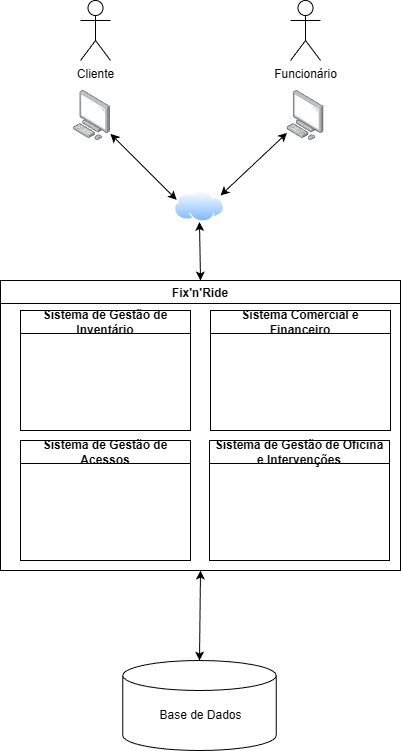
\includegraphics[scale=0.45]{images/Maqueta.png}
        \caption[Maqueta]{Maqueta}
        \label{fig:maqueta}
    \end{figure}
    
\subsection{Módulos do Sistema}
\begin{itemize}
    \item \textbf{Gestão de Inventário:} Monitoriza os níveis de \textit{stock} e gere o catálogo de peças.
    \item \textbf{Comercial e Financeiro:} Processa pagamentos, gera faturas e relatórios operacionais.
    \item \textbf{Gestão de Acessos e Utilizadores:} Garante a segurança através de perfis diferenciados para Clientes e Funcionários.
    \item \textbf{Oficina e Intervenções:} Orquestra o ciclo de vida das reparações, desde o agendamento ao levantamento.
\end{itemize}

Esta estrutura web-based permite que a informação flua em tempo real entre a oficina e a administração, eliminando os atrasos provocados por métodos manuais. 
\clearpage
\section{Diagramas de Atividades}
    Os diagramas de atividades apresentados nesta secção detalham o comportamento dinâmico do sistema, ilustrando o fluxo de controlo e de dados entre os diferentes intervenientes e a plataforma. Estes diagramas complementam a especificação de Casos de Uso, garantindo que os processos operacionais da MobiFix sejam executados de forma coerente e eficiente. 
\subsection{Fluxos de Atendimento e Diagnóstico}
O ciclo de vida de uma reparação inicia-se com o agendamento por parte do cliente, conforme ilustrado na Figura \ref{fig:agendar_diagnostico}. Após a autenticação, o utilizador seleciona uma trotinete do seu histórico e reserva uma slot disponível na agenda da oficina. 
\begin{figure}[!h]
\centering
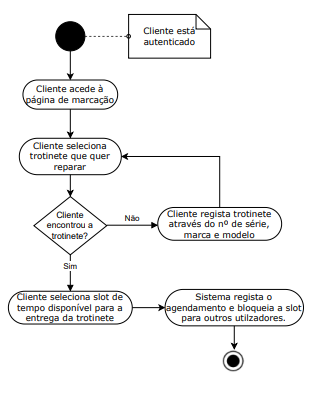
\includegraphics[scale=0.45]{images/agendar_diagnostico.png}
\caption[Agendar Diagnóstico]{Agendar Diagnóstico}
\label{fig:agendar_diagnostico}
\end{figure}

No dia agendado, ocorre o processo de triagem técnica (Figura \ref{fig:diagnostico}). O mecânico realiza o diagnóstico físico e seleciona as intervenções necessárias através do catálogo digital, o que permite ao sistema gerar automaticamente uma Guia de Reparação em formato PDF para validação do cliente. 
\begin{figure}[!h]
\centering
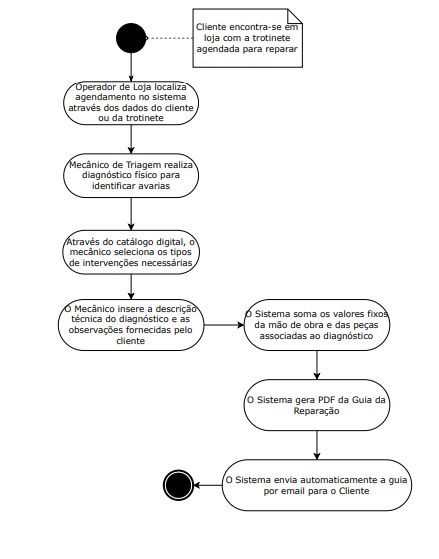
\includegraphics[scale=0.45]{images/diagnostico.png}
\caption[Diagnóstico e Geração de Guia de Reparação]{Diagnóstico e Geração de Guia de Reparação}
\label{fig:diagnostico}
\end{figure}

\clearpage
\subsection{Gestão de Inventário e Reposição}

A robustez da cadeia de abastecimento é garantida por fluxos de reposição inteligente. A Figura \ref{fig:reposicao} descreve o mecanismo de monitorização automática de stock: ao atingir o limite mínimo, o sistema cria uma encomenda com o estado "Pendente". Esta deve ser revista e aprovada pela administração (Figura \ref{fig:valida_encomenda}) para controlo financeiro antes da transição para o estado "Em Trânsito". 
\begin{figure}[!h]
\centering
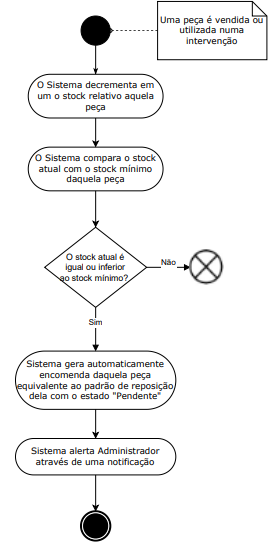
\includegraphics[scale=0.45]{images/reposicao_inteligente.png}
\caption[Encomenda de Reposição Inteligente]{Encomenda de Reposição Inteligente}
\label{fig:reposicao}
\end{figure}

\begin{figure}[!h]
\centering
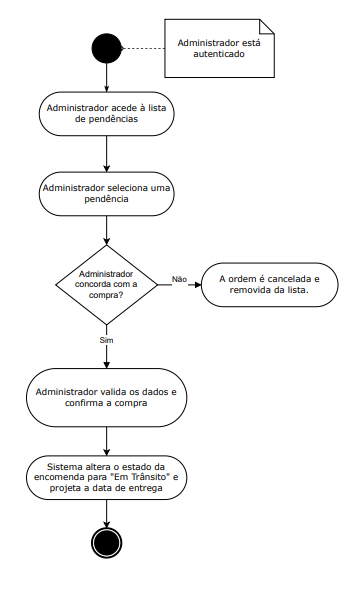
\includegraphics[scale=0.45]{images/valida_encomenda.png}
\caption[Administrador valida Encomenda]{Administrador valida Encomenda}
\label{fig:valida_encomenda}
\end{figure}

A receção física das peças pelo operador de loja (Figura \ref{fig:receciona_encomenda}) encerra o ciclo de aprovisionamento, incrementando automaticamente o inventário disponível para a oficina. 
\begin{figure}[!h]
\centering
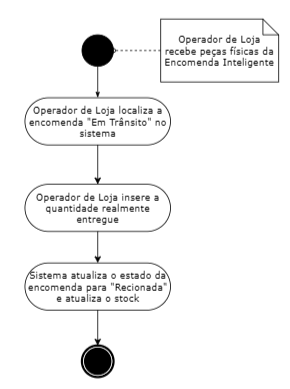
\includegraphics[scale=0.45]{images/rececao_encomenda.png}
\caption[Operador de Loja receciona encomenda]{Operador de Loja receciona encomenda}
\label{fig:receciona_encomenda}
\end{figure}

\clearpage
\subsection{Execução e Faturação}
Durante a execução da reparação (Figura \ref{fig:execução_reparaçao}), o mecânico regista os códigos únicos das peças utilizadas para garantir a rastreabilidade e as timestamps de início e fim do serviço. A conclusão de todas as tarefas aciona uma notificação automática ao cliente. 
\begin{figure}[!h]
\centering
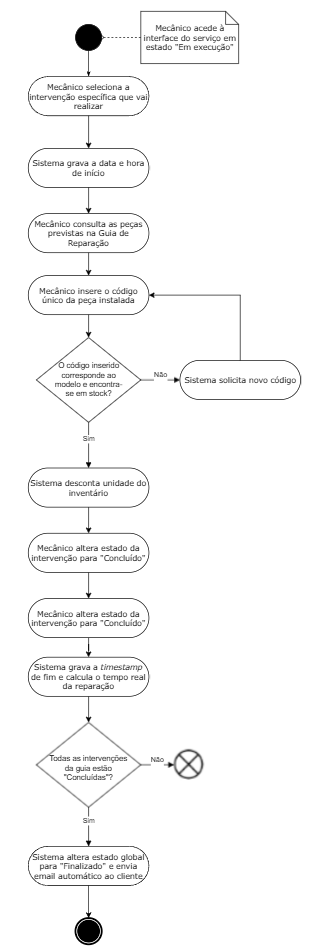
\includegraphics[scale=0.45]{images/Execução da Reparação.png}
\caption[Execução da Reparação]{Execução da Reparação}
\label{fig:execução_reparaçao}
\end{figure}

Finalmente, o sistema suporta tanto a Venda Direta ao Balcão (Figura \ref{fig:venda_direta}) quanto o levantamento de veículos reparados (Figura \ref{fig:levantamento}), assegurando a emissão das respetivas faturas e a conformidade fiscal de todas as transações. 
\begin{figure}[!h]
\centering
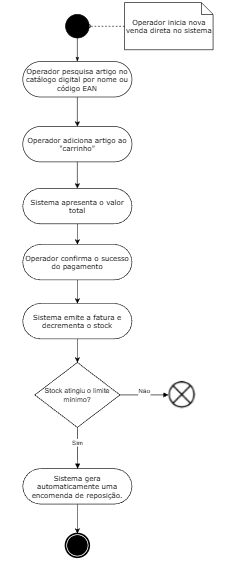
\includegraphics[scale=0.45]{images/venda_direta.png}
\caption[Venda Direta ao Balcão]{Venda Direta ao Balcão}
\label{fig:venda_direta}
\end{figure}

\begin{figure}[!h]
\centering
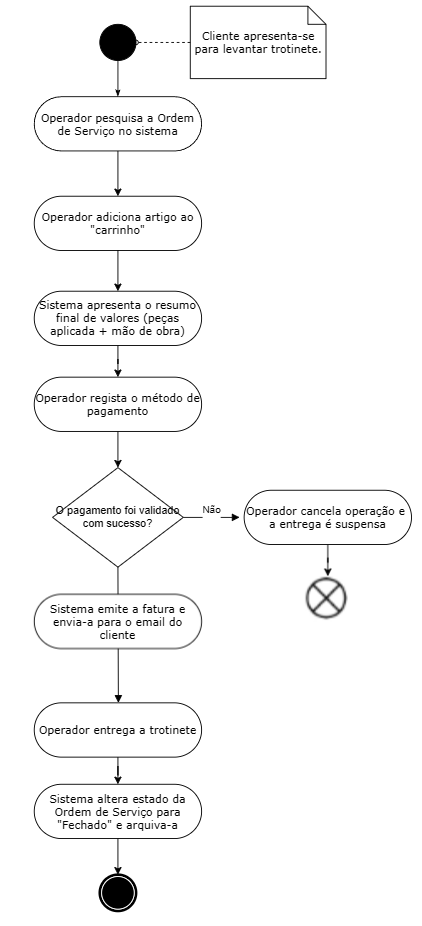
\includegraphics[scale=0.45]{images/levantamento.png}
\caption[Faturação e Levantamento da Trotinete]{Faturação e Levantamento da Trotinete}
\label{fig:levantamento}
\end{figure}

\clearpage
\section{Diagramas de Máquina de Estados}

\paragraph{}Para uma melhor compreensão do funcionamento das 3 operações-chave do sistema, recorreu-se à elaboração de Diagramas de Máquina de Estados. Estes diagramas ilustram as dinâmicas da plataforma \textit{Fix'n'Ride}, mapeando todos os estados pelos quais as principais entidades transitam desde a sua criação até à sua conclusão ou arquivo, bem como os eventos que despoletam essas transições. \paragraph{}Nesta secção, apresentam-se os modelos comportamentais de três fluxos fundamentais para a operação da \textit{MobiFix}:
\begin{itemize}
    \item \textbf{Serviço de Reparação (Ordem de Serviço):} Acompanha a jornada técnica e comercial da trotinete, iniciando-se com o agendamento do diagnóstico pelo cliente, passando pela execução mecânica na bancada, até ao estado de conclusão e posterior faturação e levantamento ao balcão.
    \item \textbf{Encomenda de Reposição (Gestão de \textit{Stock}):} Modela a cadeia de abastecimento automatizada, desde o momento em que o sistema alerta para a necessidade de repor \textit{stock} e gera uma pendência, passando pela aprovação financeira da administração para "Em Trânsito", até à atualização do inventário após a conferência da mercadoria entregue pelo fornecedor.
    \item \textbf{Encomenda de Cliente (Venda e Levantamento):} Ilustra o fluxo comercial de aquisição autónoma de peças online (\textit{Click \& Collect}), onde a encomenda transita do estado de "Pronto para Levantamento" para "Entregue" após a recolha física e verificação na loja.
\end{itemize}

\paragraph{}Abaixo encontram-se representados os respetivos diagramas que formalizam estas lógicas de transição. 
\vskip 0.5cm
\begin{figure}[H]
\centering
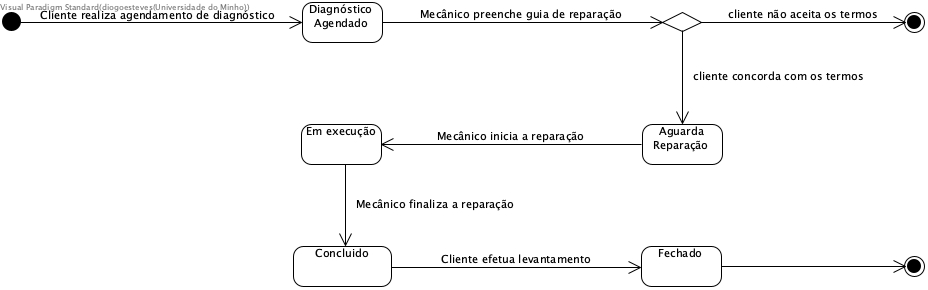
\includegraphics[scale=0.45]{images/Serviço de Reparação.jpg}
\caption[Serviço de Reparação]{Diagrama de máquina de estados do serviço de reparação}
\label{fig:levantamento}
\end{figure}


\begin{figure}[H]
\centering
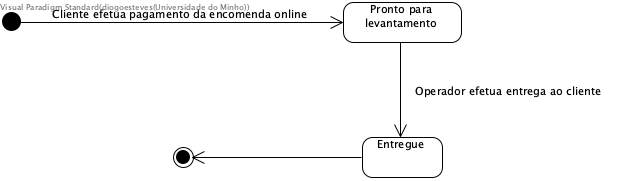
\includegraphics[scale=0.45]{images/Encomenda de Cliente.jpg}
\caption[Encomenda de cliente]{Diagrama de máquina de estados da encomenda de cliente}
\label{fig:levantamento}
\end{figure}


\begin{figure}[H]
\centering
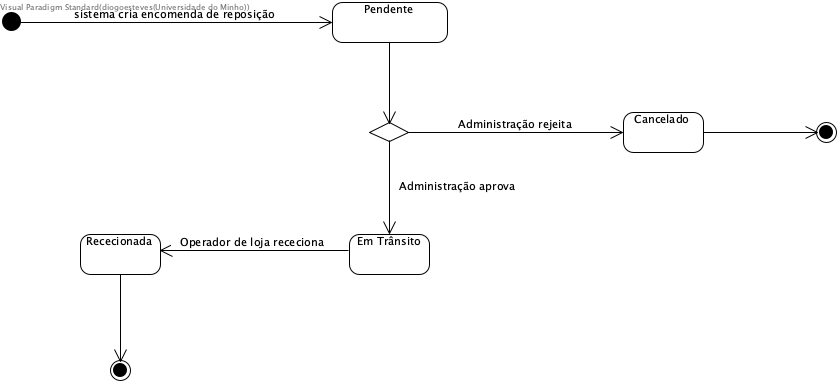
\includegraphics[scale=0.45]{images/Encomenda de Reposição.jpg}
\caption[Encomenda de Reposição]{Diagrama de máquina de estados da encomenda de reposição}
\label{fig:levantamento}
\end{figure}

\clearpage
\section{Reflexão acerca da utilização de LLMs na conceção e engenharia de requisitos do sistema Fix'N'Ride}

\paragraph{}A adoção de Grandes Modelos de Linguagem (LLMs) na primeira fase de conceção e engenharia de requisitos do sistema Fix'n'Ride assumiu um papel estrito de assistência e aceleração, e não de substituição da análise humana. É imperativo salientar que a Inteligência Artificial não foi responsável pela identificação nem pelo levantamento dos requisitos operacionais ou de negócio. A definição das regras, necessidades e restrições do sistema foi integralmente conduzida pela equipa técnica com base no estudo das operações da MobiFix. A utilização das LLMs centrou-se, exclusivamente, na agilização da materialização e documentação desse esforço analítico. \paragraph{}Neste contexto, as ferramentas de IA revelaram-se valiosas na estruturação inicial do documento, prestando apoio na geração da contextualização do projeto e na pesquisa exploratória sobre o panorama atual da micromobilidade. Foram também utilizadas para transformar as notas recolhidas pela equipa em narrativas coesas, auxiliando na redação das simulações das entrevistas aos \textit{stakeholders} e na formulação padronizada das \textit{User Stories}, garantindo que a comunicação das necessidades se mantinha clara e percetível. \paragraph{}Adicionalmente, as LLMs atuaram como um co-piloto na escrita deste capítulo, otimizando o tempo de redação. A sua capacidade de processamento de linguagem natural foi aplicada no refinamento e na articulação de parágrafos mais densos e técnicos, assegurando a coesão, a correção gramatical e o rigor vocabular exigidos num documento formal de Engenharia de Software. \paragraph{}Por fim, estabeleceu-se uma fronteira metodológica clara: não houve qualquer recurso a LLMs para o desenho ou geração dos diagramas UML, nem na identificação dos requisitos. Toda a modelação visual — incluindo o Modelo de Domínio, os Diagramas de Casos de Uso e os Diagramas de Atividades — resultou exclusivamente do esforço analítico, lógico e concetual da equipa de desenvolvimento. O levantamento dos requisitos foi realizado tendo por base o conhecimento e a observação da equipa em cenários reais, utilizando exemplos de oficinas de reparação consolidadas (como a Norauto) e procurando espelhar o seu funcionamento no contexto da micromobilidade. Esta abordagem garantiu que a espinha dorsal arquitetural do sistema Fix'n'Ride reflete fielmente as restrições da realidade, sem introduzir alucinações ou artefactos genéricos na estrutura do sistema. Os \textit{prompts} utilizados nesta etapa encontram-se no Anexo 2

\chapter{Arquitetura da Camada de Dados}
\section{Modelo Conceitual}
\subsubsection{Apresentação da Abordagem de Modelação Realizada
}
A equipa de desenvolvimento adotou uma abordagem de modelação conceptual orientada a \textbf{entidades} e \textbf{relacionamentos}. O objetivo primordial foi criar um esquema robusto, claro e coerente com os requisitos levantados para a MobiFix. Iniciou-se a elaboração deste esquema pela identificação das entidades que compõem o ecossistema da oficina, fruto de uma análise cuidada dos processos de diagnóstico e reparação. Assim, surgiram entidades nucleares como Clientes, Trotinetes, Serviços, Peças, Vendas e Funcionários — esta última especializada nos perfis de Administrador, Mecânico e Operador de Loja. Posteriormente, passou-se à definição dos atributos essenciais para caracterizar cada objeto do mundo real. Após a definição das entidades, analisaram-se os relacionamentos que regem a lógica do negócio. A associação entre Cliente e Trotinete, a relação entre Trotinete e Serviço, e a ligação entre Serviço e Peça (através das Intervenções) são exemplos vitais de relacionamentos que garantem a rastreabilidade total do histórico do veículo. As cardinalidades foram determinadas com base nas dependências operacionais, como o facto de um serviço gerar obrigatoriamente uma Guia de Reparação e, posteriormente, uma Fatura. Durante o trabalho, a equipa teve a preocupação constante em evitar a redundância e garantir a integridade dos dados, mantendo o modelo focado e alinhado com a realidade da MobiFix. Destaca-se ainda a inclusão de fluxos auxiliares, como a gestão de Promoções e o processo de Devolução, que origina a respetiva Nota de Crédito. O produto final é um modelo conceptual estruturado e ajustado às necessidades identificadas, representando de forma precisa as entidades principais e as relações essenciais ao funcionamento do futuro sistema de base de dados do Fix'n'Ride. \subsubsection{Apresentação e Explicação do Diagrama ER Produzido}

\begin{figure}[!h]
        \centering
        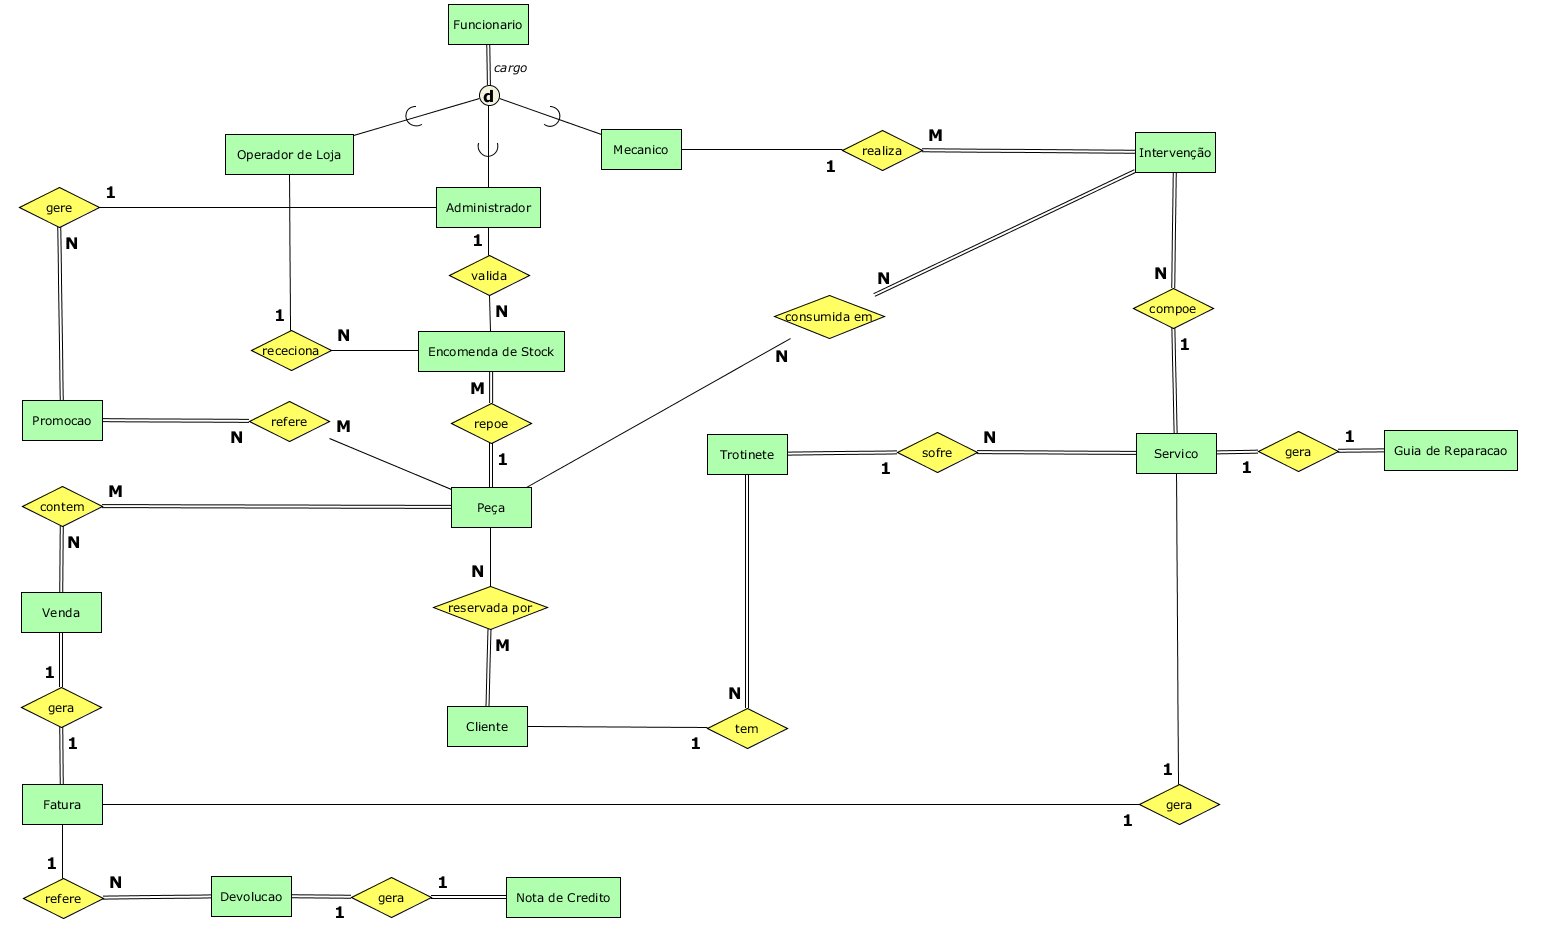
\includegraphics[scale=0.30]{images/Modelo Conceitual.png}
        \caption[Diagrama de Entidade Relacionamento]{Diagrama de Entidade Relacionamento}
        \label{fig:diagrama_er}
\end{figure}

O diagrama representado na Figura \ref{fig:diagrama_er} constitui o mapa visual e estruturado de como o novo sistema de informação da \textbf{MobiFix} irá operar. Utiliza-se a notação de Entidade-Relacionamento para identificar as entidades principais do negócio, as suas propriedades essenciais e a forma como interagem para suportar o fluxo de reparação de micromobilidade. A MobiFix gere o registo dos seus utilizadores através da entidade \textbf{Cliente}. Esta entidade inclui atributos fundamentais como o identificador único (\textit{ClienteID}), o nome, o NIF (essencial para a faturação), o contacto telefónico e o email. Além disso, a entidade Cliente estabelece uma ligação direta com os seus veículos, permitindo o acompanhamento personalizado de cada equipamento. Os colaboradores da oficina são representados pela entidade \textbf{Funcionário}, que possui uma especialização disjunta para distinguir as permissões de acesso (\textbf{RBAC}). Esta entidade especializa-se em três perfis: \textbf{Administrador} (responsável pela gestão estratégica e financeira), \textbf{Operador de Loja} (focado no atendimento ao balcão e logística) e \textbf{Mecânico} (encarregue da execução técnica). A entidade \textbf{Trotinete} destina-se a registar os veículos sujeitos a intervenção, incluindo o seu \textbf{Número de Série}, marca e modelo. Cada trotinete mantém um histórico de intervenções através da entidade \textbf{Serviço}, que monitoriza o \textbf{Estado} da reparação --- desde o agendamento até ao fecho --- e os valores associados. O núcleo técnico do sistema reside na entidade \textbf{Intervenção}, que compõe o \textbf{Serviço}. Uma intervenção é realizada por um \textbf{Mecânico} e pode consumir múltiplas unidades da entidade \textbf{Peça}. A entidade \textbf{Peça} é central para o inventário, registando o \textbf{Código EAN}, \textbf{PVP}, stock atual e o \textbf{Stock Mínimo} para alertas de reposição. No que diz respeito aos relacionamentos, o modelo estabelece as seguintes ligações:

\begin{itemize}
    \item \textbf{Tem}: Entre \textbf{Cliente} e \textbf{Trotinete}, indica que um cliente pode possuir várias trotinetes, mas cada veículo pertence a um único dono (cardinalidade \textbf{1:N}).
    \item \textbf{Sofre}: Liga \textbf{Trotinete} a \textbf{Serviço}, expressando que um veículo acumula um histórico de várias intervenções técnicas ao longo do seu ciclo de vida (\textbf{1:N}).
    \item \textbf{Gera}: Estabelece que cada \textbf{Serviço} de diagnóstico origina obrigatoriamente uma \textbf{Guia de Reparação} (\textbf{1:1}), garantindo a transparência orçamental ao cliente.
    \item \textbf{Compõe}: Interliga \textbf{Intervenção} a \textbf{Serviço} (\textbf{N:1}), permitindo que uma reparação complexa seja dividida em várias tarefas técnicas específicas.
    \item \textbf{Consumida em}: Liga \textbf{Peça} a \textbf{Intervenção} (\textbf{N:N}), rastreando exatamente quais os componentes utilizados em cada tarefa para efeitos de garantia e baixa automática de stock.
    \item \textbf{Gera (Financeiro)}: Liga tanto \textbf{Venda} como \textbf{Serviço} à entidade \textbf{Fatura} (\textbf{1:1}), assegurando a conformidade fiscal de todas as transações.
    \item \textbf{Repõe}: O fluxo de logística onde a \textbf{Peça} é vinculada a uma \textbf{Encomenda de Stock}, que deve ser validada pelo \textbf{Administrador} e rececionada pelo \textbf{Operador de Loja}.
\end{itemize}

O diagrama Entidade-Relacionamento representa a estrutura final do \textbf{Modelo Conceptual} do sistema \textbf{Fix'n'Ride}. Este modelo sintetiza os requisitos operacionais da \textbf{MobiFix}, definindo as regras que gerem os dados desde o agendamento inicial até à faturação final. A sua precisão garante que a implementação física da base de dados relacional estará perfeitamente alinhada com a necessidade de digitalização e escalabilidade da oficina. \newpage

\section{Modelo Lógico}
\subsubsection{Construção e Validação do Modelo de Dados Lógico}

No desenvolvimento da base de dados do sistema \textbf{Fix'n'Ride}, partiu-se do esquema conceptual onde foram definidas as entidades nucleares: \textbf{Cliente}, \textbf{Trotinete}, \textbf{Serviço}, \textbf{Peça}, \textbf{Funcionário} e \textbf{Fatura}. A partir deste modelo, procedeu-se à sua conversão para o respetivo esquema lógico relacional, garantindo a integridade dos fluxos de oficina e venda. Iniciou-se o processo de elaboração do esquema lógico convertendo, em primeiro lugar, cada entidade forte numa relação (tabela). Foram definidas chaves primárias (\textit{Primary Keys}) adequadas, tipicamente do tipo \texttt{INT IDENTITY} para garantir unicidade e performance, incluindo os seus atributos simples como nomes, NIF, contactos, preços e \textit{timestamps}. De seguida, tratou-se a especialização da entidade \textbf{Funcionário}. Optou-se pela estratégia de tabela única (\textit{Single Table Inheritance}), onde os perfis de \textbf{Administrador}, \textbf{Mecânico} e \textbf{Operador de Loja} são diferenciados através de um atributo de cargo e permissões de acesso (\textbf{RBAC}), otimizando a lógica de autenticação do sistema. Os relacionamentos foram convertidos seguindo as regras da modelação relacional:
\begin{itemize}
    \item \textbf{Relacionamentos 1:N}: Como \textbf{Cliente} possui \textbf{Trotinete} ou \textbf{Trotinete} sofre \textbf{Serviço}, introduziram-se chaves estrangeiras (\textit{Foreign Keys}) na tabela do lado "N" para manter a rastreabilidade.
    \item \textbf{Relacionamentos N:N}: Casos como a utilização de múltiplas \textbf{Peças} em diversas \textbf{Intervenções} exigiram a criação de tabelas intermédias (como \texttt{Intervencao\_Pecas}), que armazenam as chaves das entidades envolvidas e atributos de instância, como a quantidade utilizada.
\end{itemize}
    \begin{figure}[!h]
        \centering
        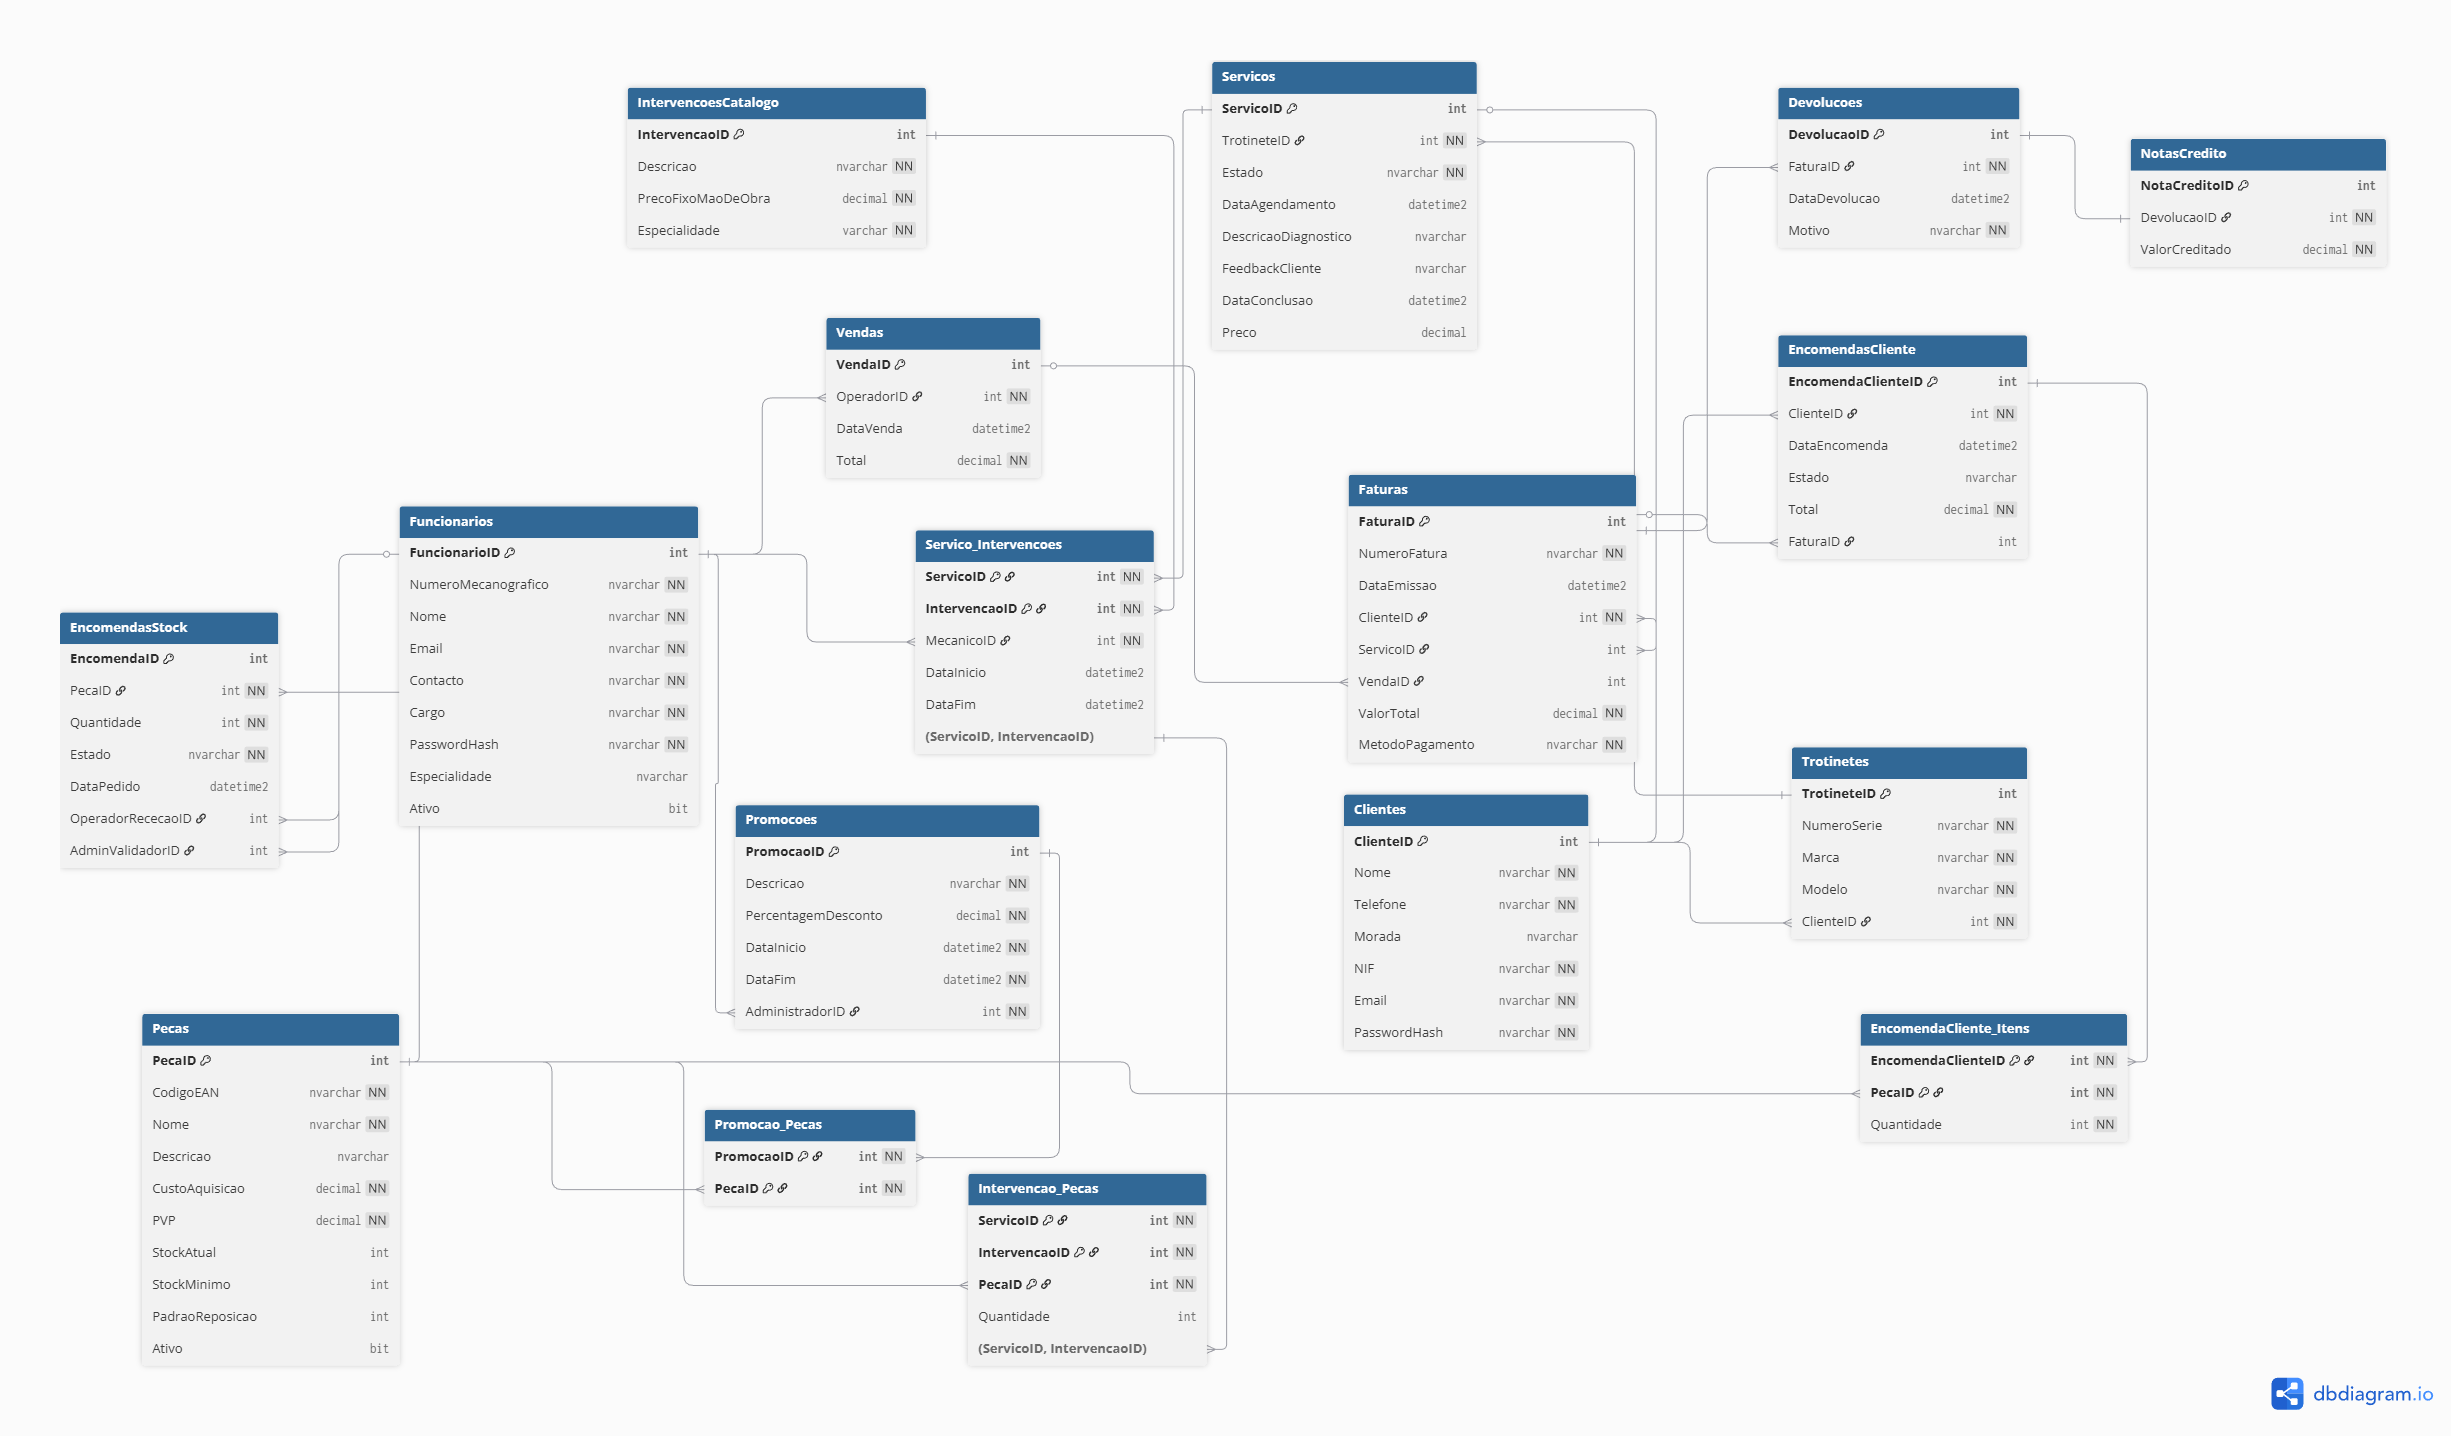
\includegraphics[scale=0.15]{images/Modelo Logico.png}
        \caption[Modelo Lógico]{Modelo Lógico}
        \label{fig:modelo_logico}
    \end{figure}
\newpage
\subsubsection{Normalização de Dados}

Com base na modelação lógica e no \textit{schema} SQL implementado, concluiu-se que a base de dados do \textbf{Fix'n'Ride} encontra-se normalizada até à \textbf{Terceira Forma Normal (3FN)}. Procedeu-se a uma inspeção sistemática para eliminar redundâncias e garantir que a estrutura suporta os requisitos funcionais da \textbf{MobiFix} sem anomalias de atualização. Para demonstrar a conformidade, analisou-se a entidade central \textbf{Serviço} (\textit{ServicoID, TrotineteID, Estado, DataAgendamento, Preco}):

\begin{enumerate}
    \item \textbf{Primeira Forma Normal (1FN)}: Todas as tabelas possuem uma chave primária definida e os atributos são atómicos. Atributos multivalorados identificados na fase conceptual, como a lista de peças associadas a uma intervenção ou itens numa promoção, foram segregados em tabelas de ligação próprias (\texttt{Intervencao\_Pecas} e \texttt{Promocao\_Pecas}).
    \item \textbf{Segunda Forma Normal (2FN)}: Verificou-se que todos os atributos não-chave dependem integralmente da chave primária. Como a chave de \textbf{Serviço} é simples (\textit{ServicoID}), evita-se qualquer dependência parcial, garantindo que o \textit{Estado} ou a \textit{Data} dependem da totalidade desse identificador.
    \item \textbf{Terceira Forma Normal (3FN)}: Confirmou-se a ausência de dependências transitivas. Na tabela \textbf{Serviço}, o \textit{TrotineteID} é uma chave estrangeira que referencia o veículo, mas não determina os restantes atributos do serviço; a lógica técnica e a temporalidade são independentes da identidade da trotinete.
\end{enumerate}

\textbf{Nota sobre Atributos Derivados}: É importante ressalvar os atributos de valor total em tabelas como \textbf{Servicos} e \textbf{Faturas}. Embora teoricamente possam ser considerados redundantes (derivados da soma de peças e mão-de-obra), optou-se por manter estes campos para otimização de performance. Esta decisão evita recálculos complexos em consultas de relatórios financeiros e históricos, sendo a integridade assegurada pela lógica de negócio no \textit{backend} .NET. Em conclusão, o esquema lógico resultante assegura uma estrutura robusta e eficiente, preparada para a escalabilidade da \textbf{MobiFix} e para a futura implementação na plataforma .NET

\subsection{Dicionário de Dados}

A presente secção detalha as especificações técnicas de cada atributo que compõe a base de dados do sistema \textbf{Fix'n'Ride}, servindo como a ponte técnica entre o modelo lógico relacional e a implementação física em \textbf{SQL Server}. O objetivo deste dicionário é garantir a integridade referencial, a consistência dos dados e o cumprimento rigoroso das regras de negócio da \textbf{MobiFix}. Cada tabela descrita abaixo funciona como a "Fonte Única de Verdade" (\textit{Single Source of Truth}) para os dados operacionais, financeiros e técnicos da oficina, assegurando que a lógica de negócio implementada em \textbf{.NET} interaja com dados devidamente tipificados e validados. Para uma melhor organização, o dicionário foi dividido em quatro módulos funcionais, seguindo a arquitetura modular do sistema. \subsubsection{Módulo 1: Gestão de Utilizadores e Controlo de Acessos}
Este módulo define a estrutura para o armazenamento de credenciais e perfis de utilizadores, suportando o sistema de controlo de acessos baseado em funções (\textbf{RBAC}). % Inserir aqui as tabelas: Funcionarios e Clientes, Trotinetes

    \begin{figure}[h]
        \centering
        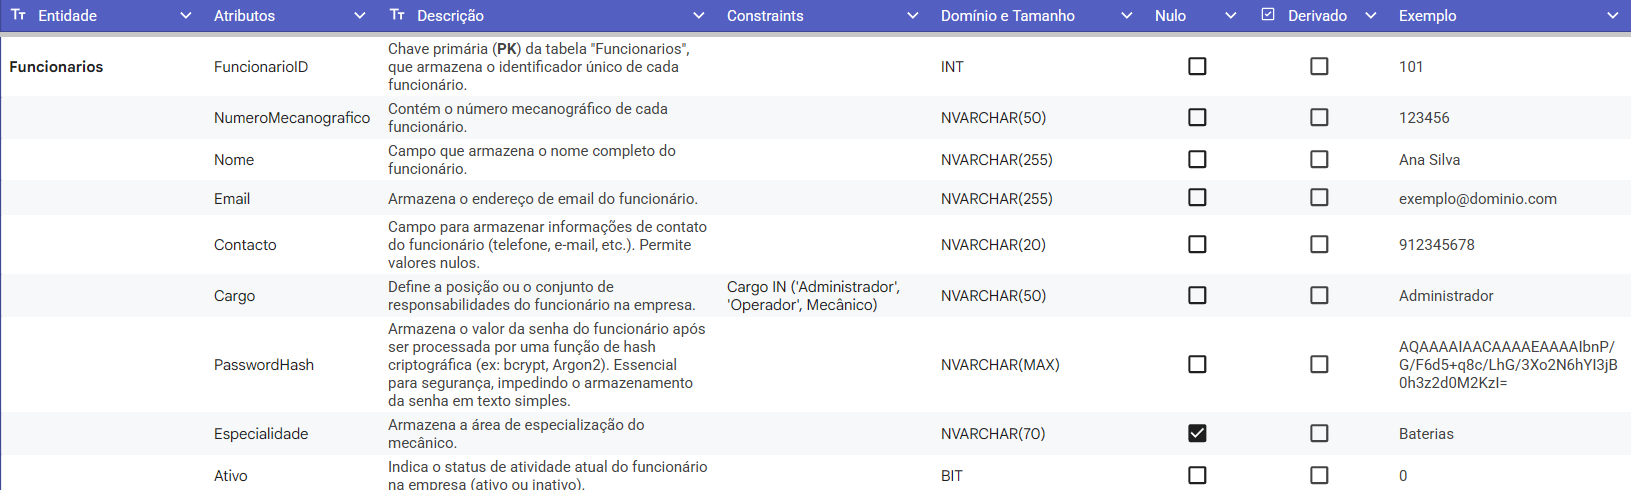
\includegraphics[scale=0.35]{images/funcionarios.png}
        \caption[Funcionários]{Funcionários}
        \label{fig:funcionarios}
    \end{figure}

    \begin{figure}[h]
        \centering
        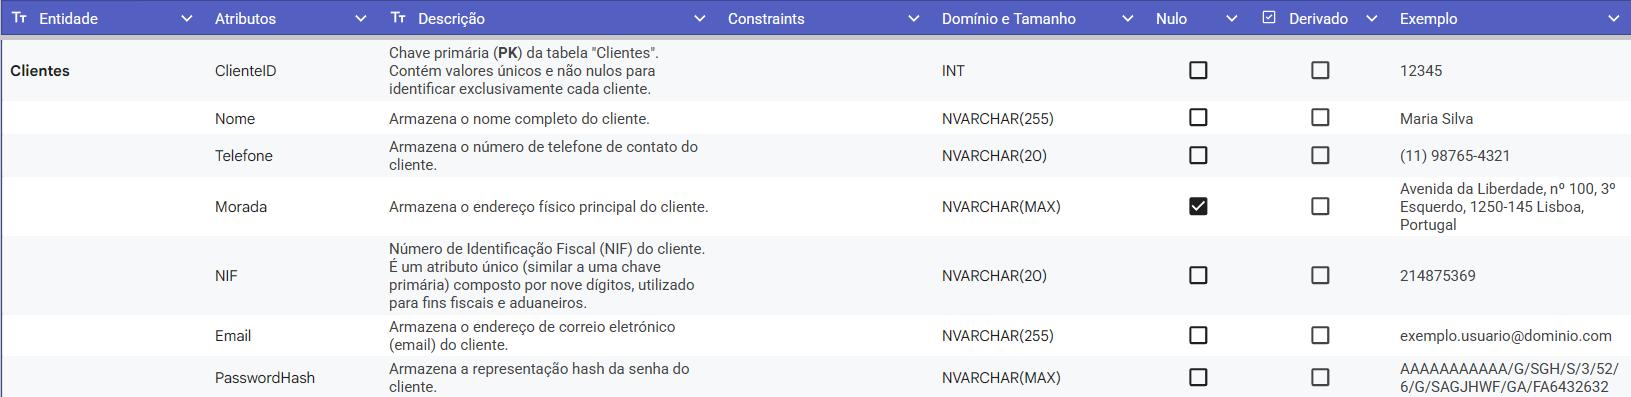
\includegraphics[scale=0.27]{images/clientes.png}
        \caption[Clientes]{Clientes}
        \label{fig:clientes}
    \end{figure}

    \begin{figure}[h]
        
\centering
        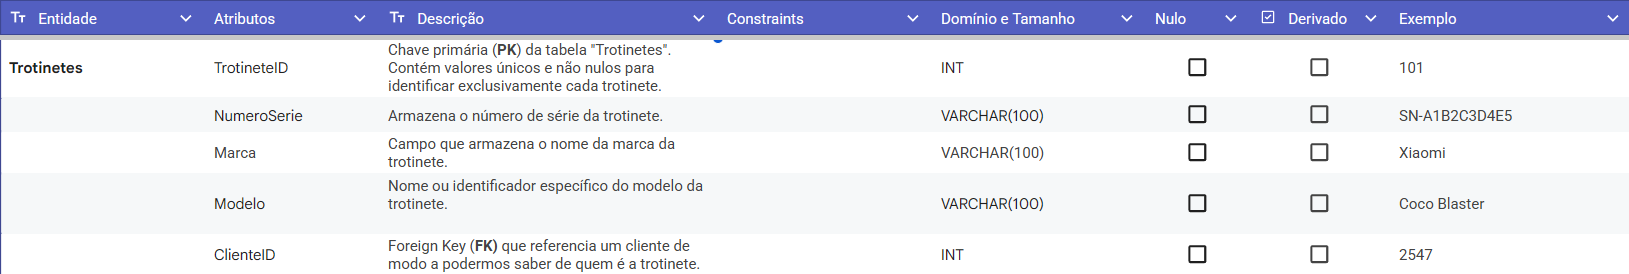
\includegraphics[scale=0.27]{images/trotinetes.png}
        \caption[Trotinetes]{Trotinetes}
        \label{fig:Trotinetes}
    \end{figure}

\subsubsection{Módulo 2: Gestão de Inventário}
Contém as definições dos veículos sob gestão e o catálogo centralizado de componentes, acessórios e intervenções técnicas pré-definidas. % Inserir aqui as tabelas: Pecas, IntervencoesCatalogo e  e EncomendasStock

    \begin{figure}[h]
        \centering
        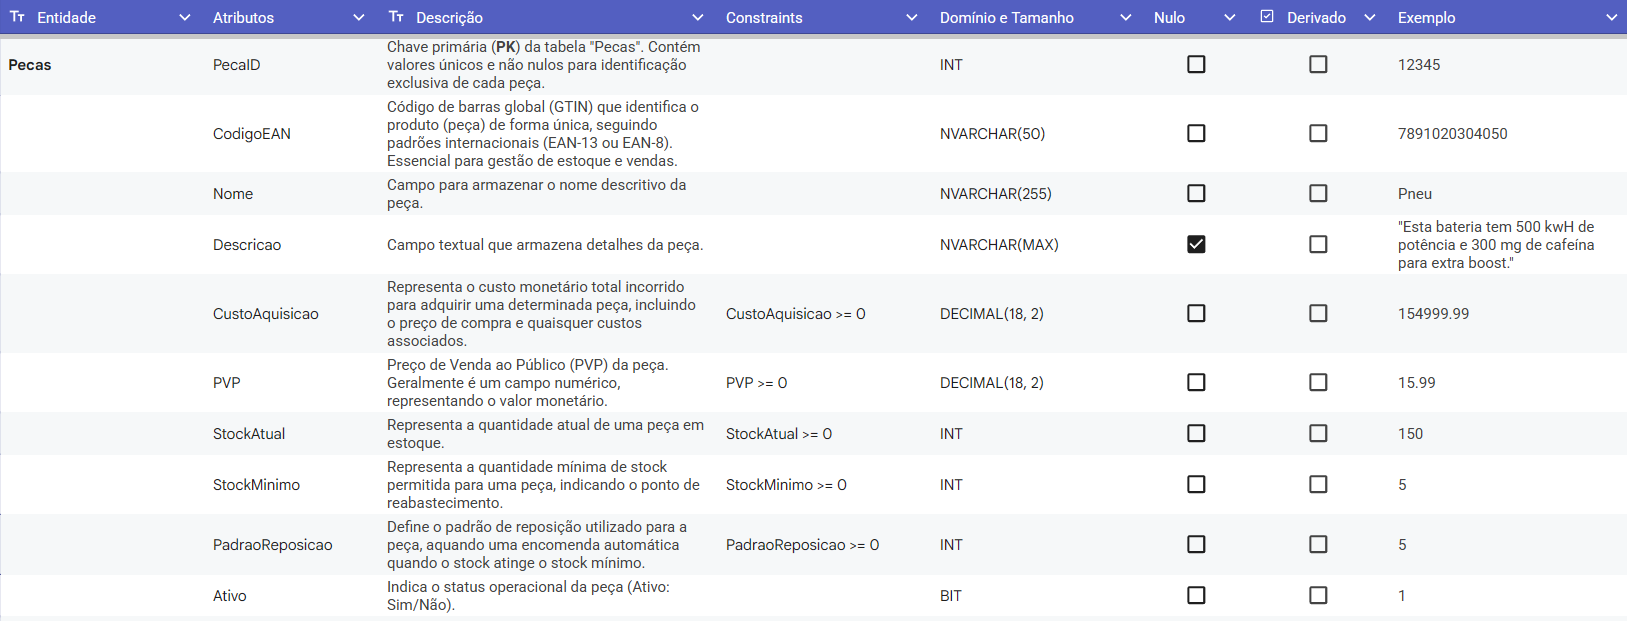
\includegraphics[scale=0.27]{images/pecas.png}
        \caption[Peças]{Peças}
        \label{fig:Peças}
    \end{figure}

    \begin{figure}[h]
        \centering
        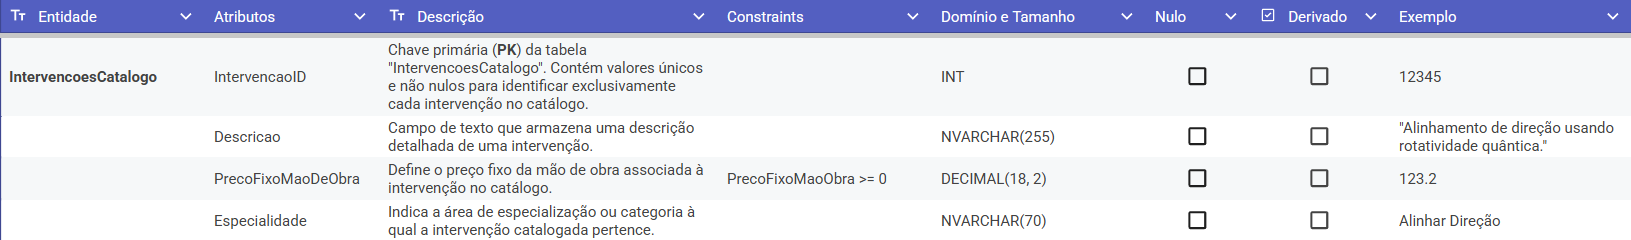
\includegraphics[scale=0.27]{images/intervencatalogo.png}
        \caption[Catálogo de Intervenções]{Catálogo de Intervenções}
        \label{fig:catalogointervencoes}
    \end{figure}

    \begin{figure}[h]
  
      \centering
        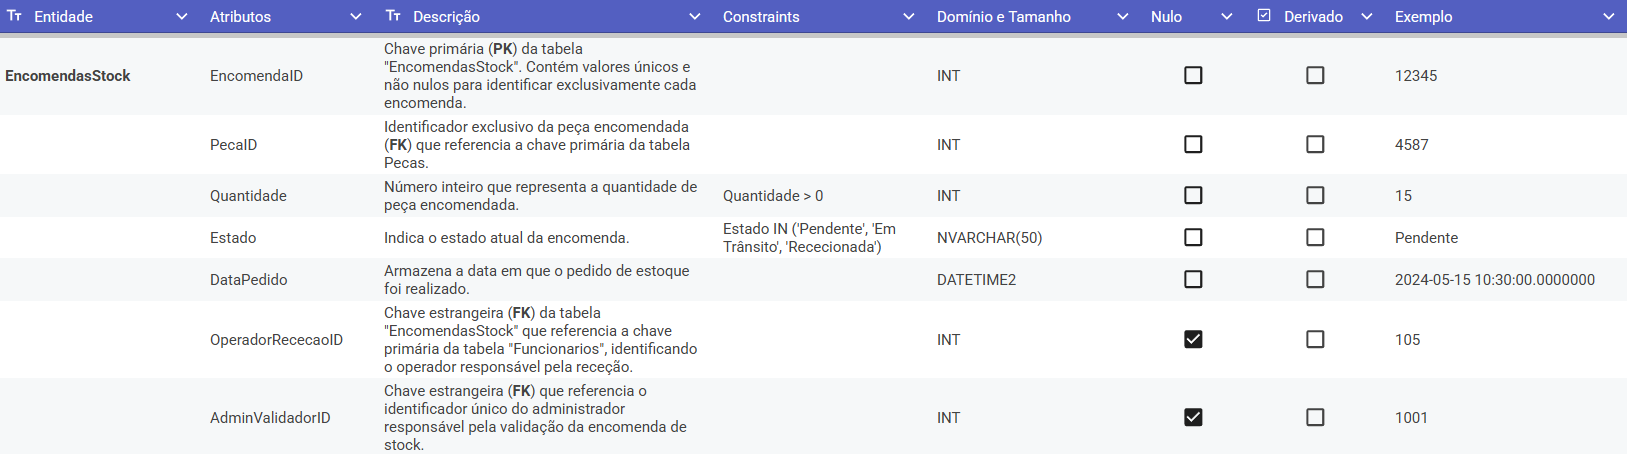
\includegraphics[scale=0.27]{images/encomendastock.png}
        \caption[Encomenda de Stock]{Encomenda de Stock}
        \label{fig:encomenda_stock}
    \end{figure}

\newpage
\subsubsection{Módulo 3: Operações de Oficina e Intervenções}
Este módulo é o núcleo operacional do sistema, registando o ciclo de vida das reparações, os diagnósticos técnicos e a alocação de recursos (mão-de-obra e peças) a cada serviço . % Inserir aqui as tabelas: Servicos, Servico_Intervencoes e Intervencao_Pecas

    \begin{figure}[h]
        \centering
        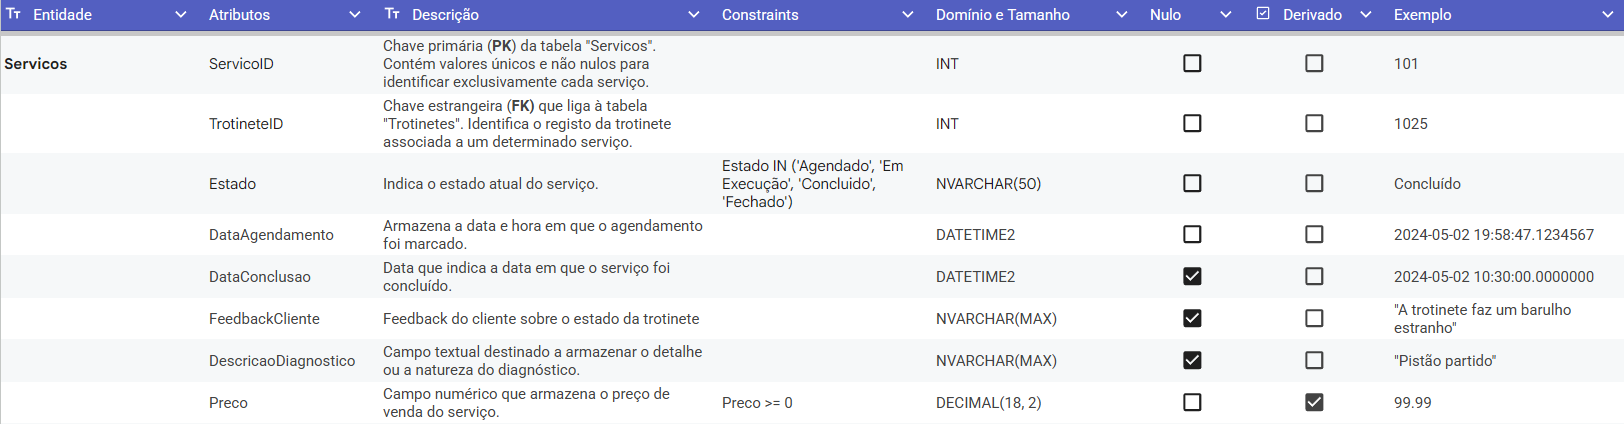
\includegraphics[scale=0.27]{images/servico.png}
        \caption[Serviço]{Serviço}
        \label{fig:servico}
    \end{figure}

    \begin{figure}[h]
        \centering
        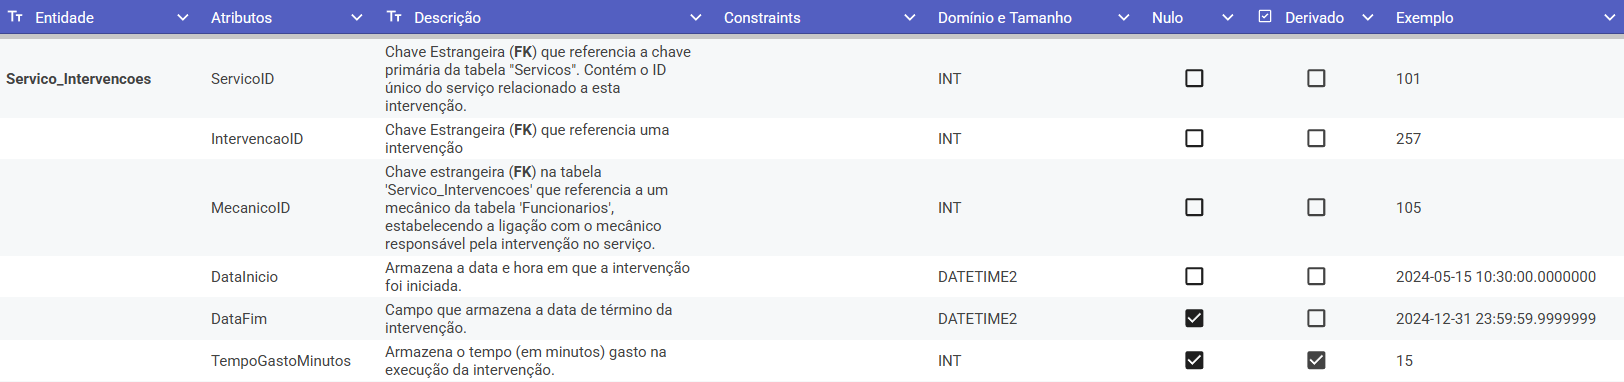
\includegraphics[scale=0.27]{images/intervencaoservico.png}
        \caption[Intervenção no Serviço]{Intervenção no Serviço}
        \label{fig:intervencao_no_servico}
    \end{figure}

    \begin{figure}[h]
    
    \centering
        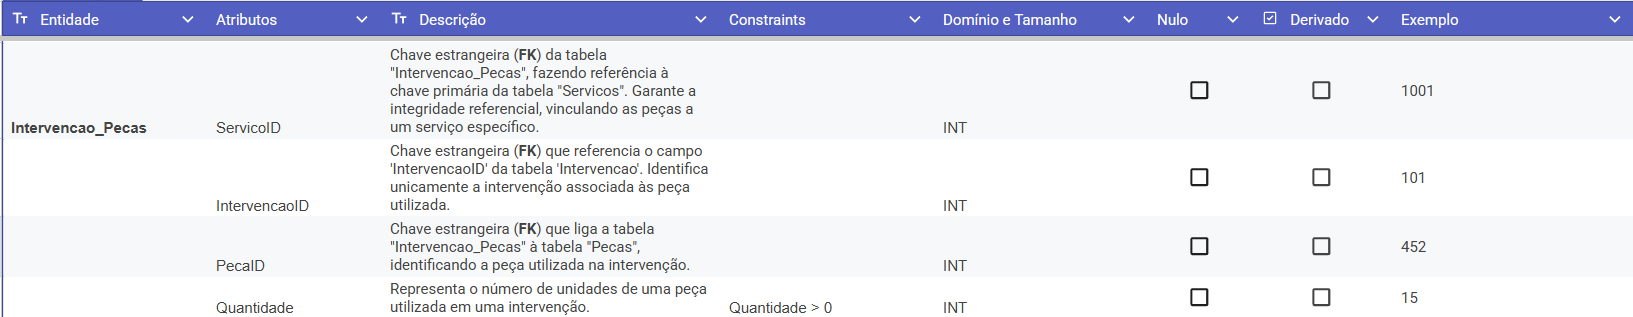
\includegraphics[scale=0.35]{images/intervencaopecas.png}
        \caption[Peça utilizada na intervenção]{Peça utilizada na Intervenção}
        \label{fig:intervencao_no_servico}
    \end{figure}

\newpage
\subsubsection{Módulo 4: Gestão Comercial e Financeira}
Define a estrutura para o registo de vendas diretas, encomendas de clientes (\textit{Click \& Collect}), faturação, notas de crédito e gestão de campanhas promocionais. % Inserir aqui as tabelas: Vendas, Faturas, Devolucoes, NotasCredito, Promocoes e EncomendasCliente

    \begin{figure}[H]
        \centering
        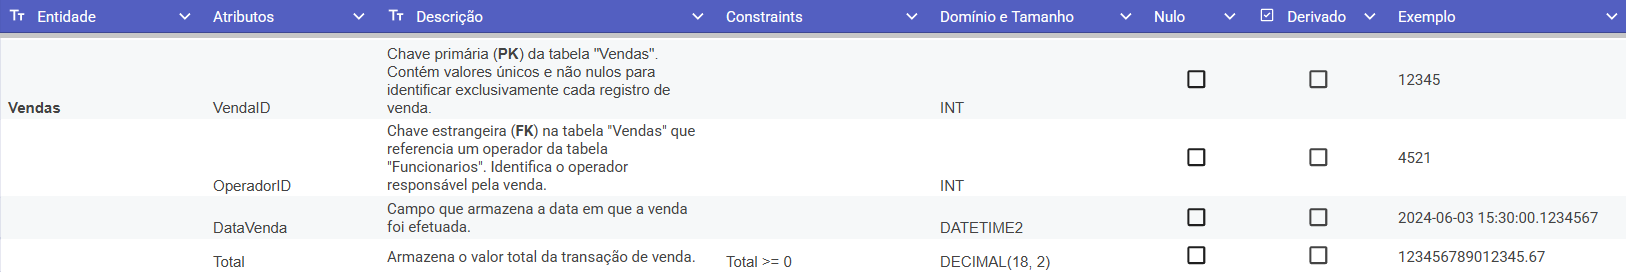
\includegraphics[scale=0.26]{images/venad.png}
        \caption[Venda]{Venda}
        \label{fig:intervencao_no_servico}
    \end{figure}

    \begin{figure}[H]
        \centering
        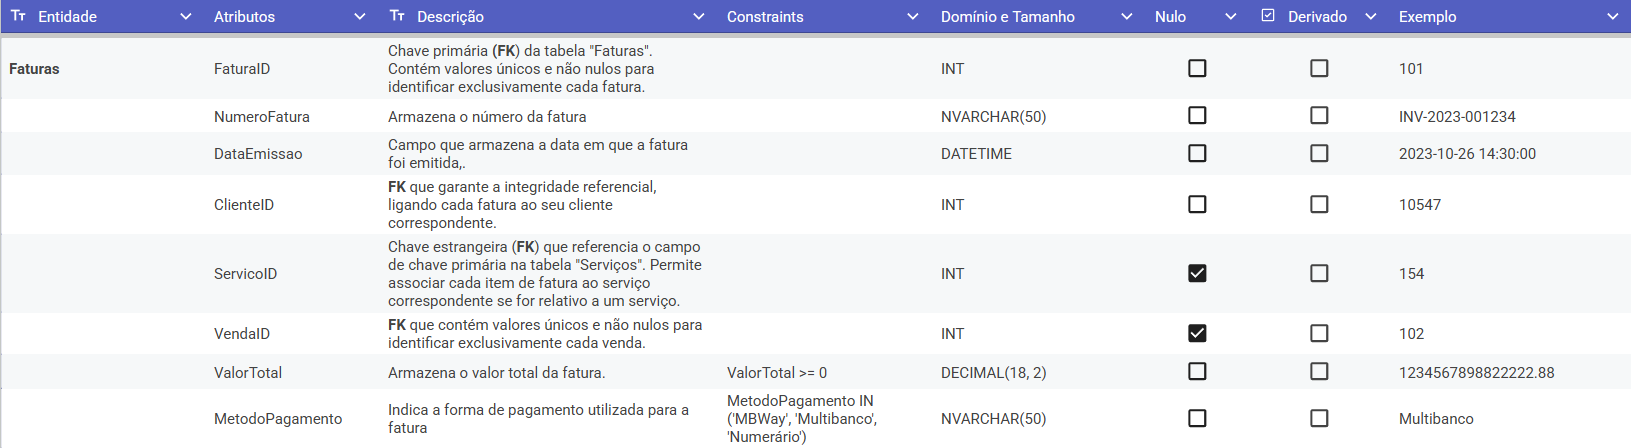
\includegraphics[scale=0.26]{images/fatura.png}
        \caption[Fatura]{Fatura}
        \label{fig:intervencao_no_servico}
    \end{figure}

    \begin{figure}[H]
     
   \centering
        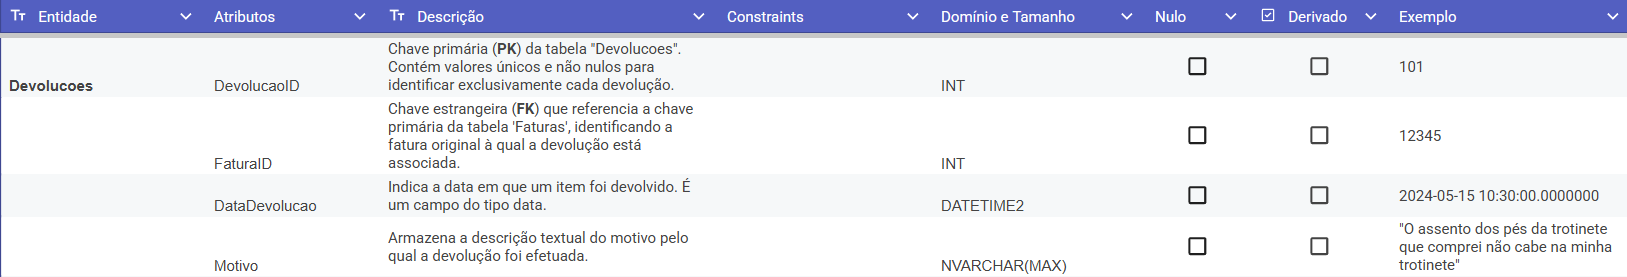
\includegraphics[scale=0.26]{images/devolucao.png}
        \caption[Devolução]{Devolução}
        \label{fig:intervencao_no_servico}
    \end{figure}

    \begin{figure}[h]
        \centering
        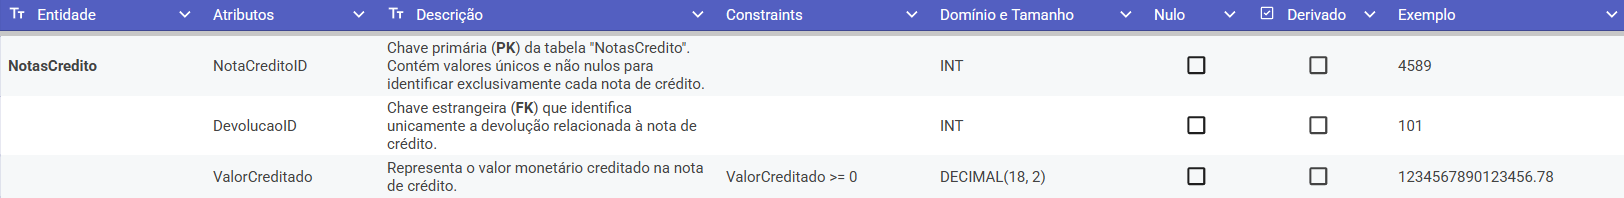
\includegraphics[scale=0.26]{images/notacredito.png}
        \caption[Nota de Crédito]{Nota de Crédito}
        \label{fig:intervencao_no_servico}
    \end{figure}

    \begin{figure}[H]
        \centering
        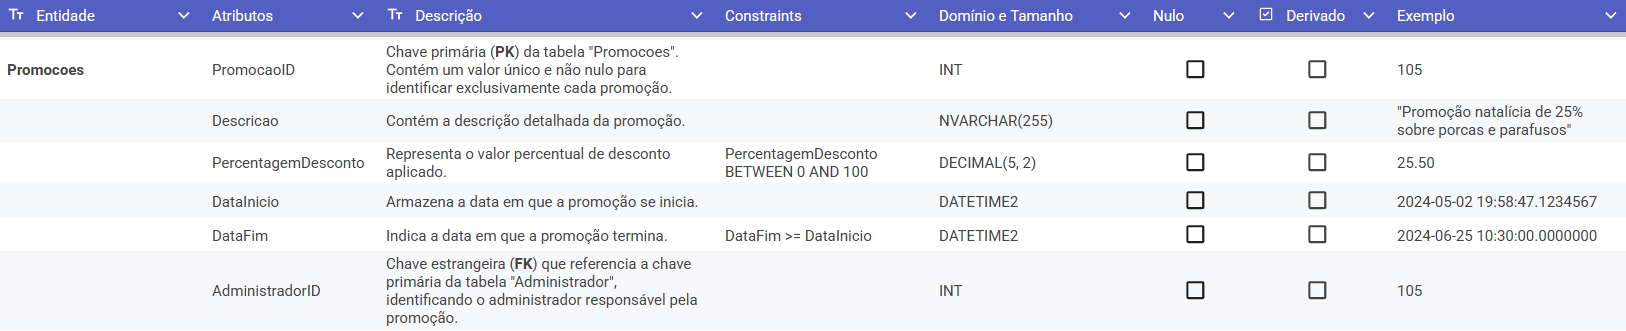
\includegraphics[scale=0.26]{images/promocao.png}
     
   \caption[Promoção]{Promoção}
        \label{fig:intervencao_no_servico}
    \end{figure}

    \begin{figure}[H]
        \centering
        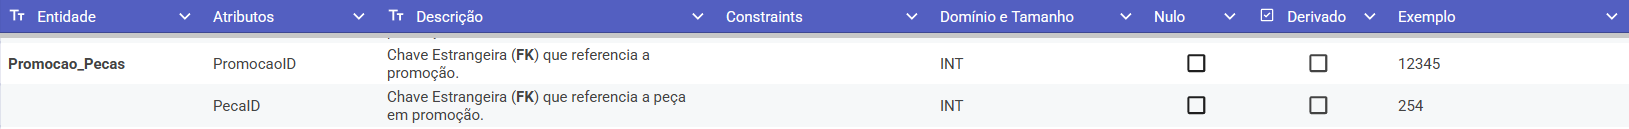
\includegraphics[scale=0.26]{images/pecaempromocao.png}
        \caption[Peças em Promoção]{Peças em Promoção}
        \label{fig:intervencao_no_servico}
    \end{figure}

    \begin{figure}[H]
        \centering
        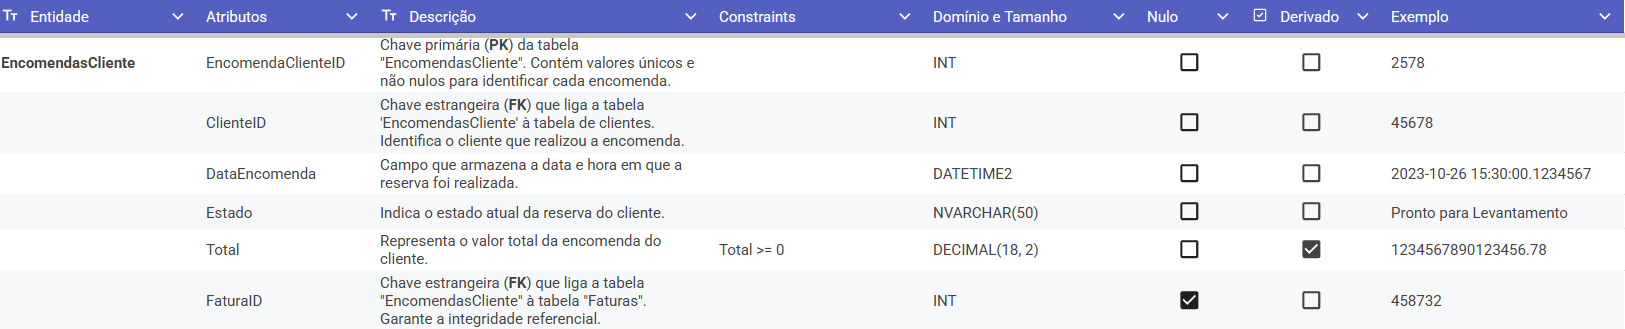
\includegraphics[scale=0.26]{images/encomendacliente.png}
        \caption[Reserva de Peça]{Reserva de Peças}
        \label{fig:intervencao_no_servico}
 
   \end{figure}
    
    \begin{figure}[H]
        \centering
        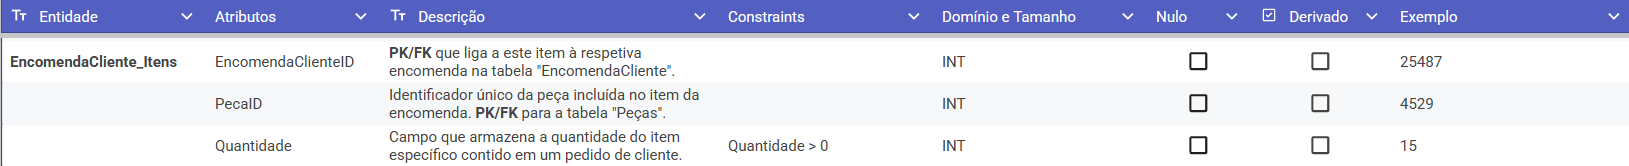
\includegraphics[scale=0.26]{images/itemsreserva.png}
        \caption[Peças reservadas]{Peças Reservadas pelo Cliente}
        \label{fig:intervencao_no_servico}
    \end{figure}


    
\newpage
\subsection{Decisões de Persistência e Tecnologia}
Nesta fase do projeto, foram consolidadas decisões arquiteturais críticas para assegurar que a infraestrutura de dados do sistema \textbf{Fix'n'Ride} suporte a escalabilidade e o rigor operacional exigidos pela \textbf{MobiFix}. A transição de um sistema fragmentado em folhas de cálculo para uma solução centralizada exige uma base tecnológica que garanta a unicidade e integridade da informação. \subsubsection{Sistema de Gestão de Base de Dados (SGBD)}
Optou-se pela utilização do \textbf{SQL Server} como motor de persistência relacional. Esta escolha é fundamental para garantir a integridade transacional e a consistência absoluta dos dados (propriedades ACID), especialmente em fluxos críticos onde a sincronização entre o inventário de peças e a faturação de serviços é vital.Concretamente, a utilização do SQL Server permite orquestrar operações complexas, como o decremento automático do \texttt{StockAtual} na tabela \texttt{Pecas} no momento em que um mecânico finaliza uma intervenção ou um operador realiza uma venda direta, prevenindo ruturas de stock e inconsistências financeiras. Além disso, o motor providencia mecanismos robustos para auditoria e recuperação de desastres, essenciais para a continuidade do negócio.\subsubsection{Camada de Abstração: .NET Data API Builder (DAB)}
Para otimizar a comunicação entre a interface \textbf{React} e o servidor de dados, implementou-se o \textbf{.NET Data API Builder (DAB)}. O DAB atua como um motor de reflexão que traduz os pedidos da lógica aplicacional em \textit{queries} SQL altamente otimizadas, expondo o esquema relacional de forma segura através de uma API REST/GraphQL.Esta decisão é estratégica para cumprir o requisito não funcional de desempenho, garantindo que o tempo de resposta em operações de leitura, como a listagem do catálogo ou consulta de histórico, não exceda os 2 segundos. Ao utilizar o DAB, minimiza-se a necessidade de código \textit{boilerplate} para acesso a dados, permitindo que a equipa se foque na implementação das regras de negócio complexas no \textit{backend} .NET.\subsubsection{Integridade e Segurança da Informação}
A persistência foi desenhada seguindo o princípio da \textit{Defense in Depth}, aplicando controlos em múltiplas camadas:

\begin{itemize}
\item \textbf{Restrições Físicas (Check Constraints)}: O \textit{schema} SQL implementa validações rigorosas a nível de tabela para impedir estados inválidos. Exemplos concretos incluem as restrições que garantem que quantidades e valores monetários nunca assumam valores negativos, e a que obriga as ordens de serviço a seguir o fluxo definido: Agendado, Em Execução, Concluido ou Fechado.
\item \textbf{Controlo de Acessos (RBAC)}: A segurança é gerida através de \textit{Role-Based Access Control}, utilizando o campo \texttt{Cargo} na tabela \texttt{Funcionarios} para segregar permissões entre \textit{Administrador}, \textit{Operador} e \textit{Mecanico}. Isto garante que, por exemplo, apenas administradores tenham acesso a relatórios financeiros e à aprovação de encomendas de reposição.
\item \textbf{Cifragem e Proteção de Dados}: Seguindo as normas de segurança do ecossistema .NET, as credenciais dos utilizadores são armazenadas na coluna \texttt{PasswordHash} através de algoritmos de \textit{hashing} irreversíveis, impedindo a exposição de palavras-passe em texto limpo mesmo em caso de acesso indevido à base de dados.
\end{itemize}

\subsection{Especificação da API}
A API do sistema \textbf{Fix'n'Ride} foi desenhada para servir de ponte robusta entre o \textit{frontend} React e a base de dados SQL Server, utilizando as capacidades de reflexão de esquema do \textit{.NET Data API Builder} (DAB). Esta abordagem permite expor os dados via REST e GraphQL de forma imediata e segura. \subsubsection{Catálogo de Recursos e Operações}
A API expõe os recursos de forma granular, permitindo operações \textit{CRUD} (Create, Read, Update, Delete) mapeadas nos fluxos de negócio:

\begin{itemize}
    \item \textbf{Módulo de Oficina}:
        \begin{itemize}
            \item \texttt{GET /api/Servicos}: Consulta de ordens de serviço (filtravel por estado ou mecânico).
            \item \texttt{PATCH /api/Servicos/\{id\}}: Atualização de estado (ex: de 'Em Execução' para 'Concluido').
            \item \texttt{POST /api/Intervencao\_Pecas}: Registo de peças consumidas numa reparação específica.
        \end{itemize}
    \item \textbf{Módulo de Inventário e Vendas}:
        \begin{itemize}
            \item \texttt{GET /api/Pecas}: Catálogo de peças com stock em tempo real.
            \item \texttt{POST /api/Vendas}: Registo de venda direta ao balcão e emissão de fatura.
            \item \texttt{PUT /api/Pecas/\{id\}}: Ajuste de stock ou preço (restrito a Administradores).
        \end{itemize}
    \item \textbf{Módulo de Gestão de Frota e Clientes}:
        \begin{itemize}
            \item \texttt{GET /api/Trotinetes}: Listagem de veículos associados a um NIF de cliente.
            \item \texttt{POST /api/Clientes}: Registo de novos utilizadores no portal MobiFix.
        \end{itemize}
\end{itemize}

\subsubsection{Políticas de Segurança e Controlo de Acesso (RBAC)}
A segurança da API é gerida diretamente no motor do DAB, onde são definidas regras de autorização baseadas nos cargos (\textit{roles}) mapeados na base de dados. Estas regras garantem o cumprimento do princípio do menor privilégio:

\begin{table}[h!]
\centering
\begin{tabular}{|l|l|l|}
\hline
\textbf{Perfil (Role)} & \textbf{Recursos Acessíveis} & \textbf{Operações Permitidas} \\ \hline
Administrador & Todos & CRUD Total, Gestão de Staff e Preçários \\ \hline
Operador & Clientes, Vendas, Faturas & Registo de Vendas, Check-in de Trotinetes \\ \hline
Mecânico & Serviços, Peças, Catálogo & Consulta de Peças, Update de Intervenções \\ \hline
Cliente & Perfil Próprio, Reservas & Consulta de Histórico e Agendamento \\ \hline
\end{tabular}
\caption{Matriz de Controlo de Acessos (RBAC) da API}
\end{table}

\subsubsection{Integridade e Contratos de Dados}
Os dados são transferidos em formato \textbf{JSON}. A API atua como um validador de primeira linha:
\begin{enumerate}
    \item \textbf{Tipagem Estrita}: O DAB garante que os campos enviados (ex: \texttt{Total} da fatura) correspondem aos tipos decimais definidos no \textit{schema}.
    \item \textbf{Respeito por Constraints}: Qualquer tentativa de inserir uma quantidade negativa via \texttt{POST /api/Pecas} é rejeitada pela API, uma vez que esta herda a restrição \texttt{CK\_Peca\_Stock} do SQL Server.
    \item \textbf{Filtragem de Campos}: Para perfis não administrativos, a API é configurada para omitir campos sensíveis (ex: \texttt{PasswordHash} ou \texttt{PrecoCusto}) nas respostas JSON.
\end{enumerate}

\chapter{Arquitetura da Lógica de Negócios}

A camada de Lógica de Negócios (LN) constitui o núcleo do sistema \textbf{Fix'n'Ride}. Enquanto o \textit{Data API Builder} (DAB) assegura a eficiência das operações básicas de leitura e escrita na base de dados, a LN, desenvolvida no ecossistema \textbf{.NET}, assume a responsabilidade exclusiva pela orquestração de transações complexas, validação de regras de negócio, cálculos financeiros e processos assíncronos (como a geração de faturas e o envio de emails). Esta abordagem garante que a aplicação seja simultaneamente performante nas consultas e estritamente rigorosa nas suas operações críticas.

\section{Visão Geral e Diagrama de Componentes}

Para dominar a complexidade do ecossistema da \textbf{MobiFix}, a arquitetura desta camada foi desenhada segundo o padrão estrutural \textit{Facade} (Fachada), conjugado com uma forte separação de responsabilidades (modularidade). 

O sistema expõe um ponto de entrada centralizado para o cliente (a classe \texttt{MobiFixService}), que abstrai a complexidade interna e delega as operações para serviços especialistas, dedicados a cada domínio do problema.

    \begin{figure}[H]
        \centering
        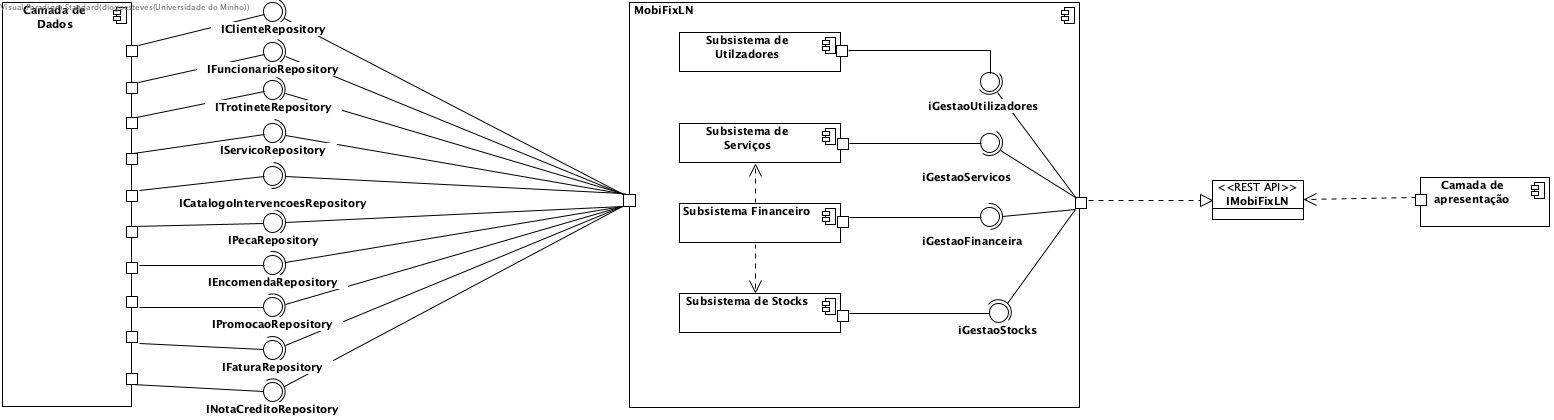
\includegraphics[scale=0.26]{images/Diagrama de Componentes Lógica de Negócios.jpg}
        \caption[Diagrama de Componentes da LN]{Diagrama de Componentes da LN}
        \label{fig:intervencao_no_servico}
    \end{figure}

A estrutura de componentes da Lógica de Negócios organiza-se da seguinte forma:

\begin{itemize}
    \item \textbf{\textit{Facade} Principal (\texttt{MobiFixService})}: Atua como o orquestrador do sistema. Recebe os pedidos complexos provenientes do \textit{frontend} (React) e encaminha-os para os respetivos gestores de domínio. Esta interface única reduz o acoplamento entre a camada de apresentação e a complexidade lógica interna.
    
    \item \textbf{Módulo de Serviços (\texttt{ServicosService})}: Encapsula as regras relativas às operações de oficina. Gere as transições de estado das ordens de serviço, associa o consumo de peças a intervenções específicas e orquestra a notificação dos clientes aquando da conclusão das reparações.
    
    \item \textbf{Módulo Financeiro (\texttt{FinancasService})}: Centraliza toda a inteligência comercial do sistema. É responsável por processar as vendas diretas ao balcão, calcular orçamentos com base no catálogo em vigor, gerar documentos fiscais rigorosos (Faturas e Notas de Crédito) e aplicar lógicas de devolução.
    
    \item \textbf{Módulo de \textit{Stocks} (\texttt{StocksService})}: Garante a integridade do inventário físico e digital. Executa a dedução de peças após validação de vendas ou reparações, e gere o fluxo de aprovação de encomendas de reposição criadas automaticamente pelo sistema.
    
    \item \textbf{Módulo de Utilizadores (\texttt{UtilizadoresService})}: Assegura a gestão de identidade. Verifica credenciais através da comparação segura de \textit{hashes}, gere a associação de novos veículos (trotinetes) ao perfil dos clientes e garante o rigor na atualização de dados pessoais e permissões.
\end{itemize}

Esta modularização não só facilita a testabilidade e manutenção do código \textbf{.NET}, como também permite que os diferentes serviços interajam de forma limpa antes de consolidarem o estado final na base de dados \textbf{SQL Server}.

\section{Módulo de Utilizadores}
\section{Módulo de Serviços}
\section{Módulo Financeiro}
\section{Módulo de Stocks}
\section{Visão Geral da Lógica de Negócios}

\section{Rotas do Servidor de Lógica de Negócios (Facade \textit{MobiFixService}):}
\paragraph{} Para expôr a lógica de negócios ao servidor web, responsável pela camada de apresentação,  
\begin{itemize}
    \item \textbf{Módulo de Gestão de Utilizadores}:
        \begin{itemize}
            \item \texttt{POST /api/logic/utilizadores/login}: Autenticação no sistema validando as credenciais do utilizador (\texttt{efetuarLogin}).
        \end{itemize}
    \item \textbf{Módulo de Gestão de Serviços}:
        \begin{itemize}
            \item \texttt{GET /api/logic/servicos/agenda}: Consulta das marcações e entregas agendadas filtradas por uma data específica (\texttt{consultarAgendaOficina}).
            \item \texttt{POST /api/logic/servicos/\{idServico\}/pecas}: Registo do código identificador de uma peça física efetivamente consumida numa reparação, deduzindo o stock (\texttt{registarPecaUtilizada}).
        \end{itemize}
    \item \textbf{Módulo de Gestão Financeira}:
        \begin{itemize}
            \item \texttt{POST /api/logic/financeira/vendas}: Registo de venda direta ao balcão com base numa lista de códigos de peças e no ID do cliente (\texttt{realizarVendaDireta}).
            \item \texttt{POST /api/logic/financeira/faturas/servico/\{idServico\}}: Emissão de fatura correspondente a um serviço concluído, retornando o documento em formato \textit{byte array} (PDF) (\texttt{faturarServico}).
            \item \texttt{POST /api/logic/financeira/devolucoes}: Processamento de devolução total ou parcial com base no ID da fatura original e nos artigos a devolver (\texttt{processarDevolucao}).
        \end{itemize}
    \item \textbf{Módulo de Gestão de Stocks}:
        \begin{itemize}
            \item \texttt{PATCH /api/logic/stocks/encomendas/\{idEncomenda\}/aprovar}: Validação e aprovação de uma encomenda de reposição que se encontre pendente (\texttt{aprovarEncomendaPendente}).
        \end{itemize}
\end{itemize}

\chapter{Camada de Apresentação}
\section{Prototipagem das Páginas Web}
\section{Definição das rotas}

\chapter{Orquestração dos Servidores e Micro-Serviços}
\paragraph{}Explicação do Docker e ENVS
\renewcommand{\nomname}{Lista de Siglas e Acrónimos}

% Tecnologias e Desenvolvimento
\nomenclature[01]{\textbf{LLM}}{\textit{Large Language Model} }
\nomenclature[02]{\textbf{SQL}}{\textit{Structured Query Language} }
\nomenclature[02]{\textbf{LN}}{\textit{Lógica de Negócios} }
\nomenclature[03]{\textbf{.NET}}{\textit{Framework de desenvolvimento da Microsoft} }
\nomenclature[04]{\textbf{C\#}}{\textit{Linguagem de programação orientada a objetos} }
\nomenclature[05]{\textbf{UML}}{\textit{Unified Modeling Language} }
\nomenclature[06]{\textbf{BD}}{\textit{Base de Dados} }
\nomenclature[07]{\textbf{API}}{\textit{Application Programming Interface} }
\nomenclature[08]{\textbf{SPA}}{\textit{Single Page Application} }
\nomenclature[09]{\textbf{CSS}}{\textit{Cascading Style Sheets} }

% Engenharia de Requisitos
\nomenclature[10]{\textbf{OS}}{\textit{Ordem de Serviço} }
\nomenclature[11]{\textbf{US}}{\textit{User Story} }
\nomenclature[12]{\textbf{UC}}{\textit{Use Case} }
\nomenclature[13]{\textbf{RF}}{\textit{Requisito Funcional} }
\nomenclature[14]{\textbf{RNF}}{\textit{Requisito Não Funcional} }
\nomenclature[15]{\textbf{RBAC}}{\textit{Role-Based Access Control} }
\nomenclature[16]{\textbf{SRS}}{\textit{Software Requirements Specification} }

% Negócio e Legislação
\nomenclature[17]{\textbf{ROI}}{\textit{Return on Investment} }
\nomenclature[18]{\textbf{OPEX}}{\textit{Operating Expenses} }
\nomenclature[19]{\textbf{NIF}}{\textit{Número de Identificação Fiscal} }
\nomenclature[20]{\textbf{PVP}}{\textit{Preço de Venda ao Público} }
\nomenclature[21]{\textbf{KPI}}{\textit{Key Performance Indicator} }
\nomenclature[22]{\textbf{EAN}}{\textit{European Article Number} }
\nomenclature[23]{\textbf{RGPD}}{\textit{Regulamento Geral sobre a Proteção de Dados} }

% Protocolos e Formatos
\nomenclature[24]{\textbf{PDF}}{\textit{Portable Document Format} }
\nomenclature[25]{\textbf{CSV}}{\textit{Comma-Separated Values} }
\nomenclature[26]{\textbf{SMTP}}{\textit{Simple Mail 
Transfer Protocol} }
\nomenclature[27]{\textbf{\textit{MBWay}}}{\textit{Sistema de pagamento eletrónico} }
\printnomenclature

\addchap{Anexos}
\addsec{Anexo 1 - Modelo de Domínio Completo} \label{anexo:modelo_dominio_BIG}
\begin{figure}[!h]
    \centering
    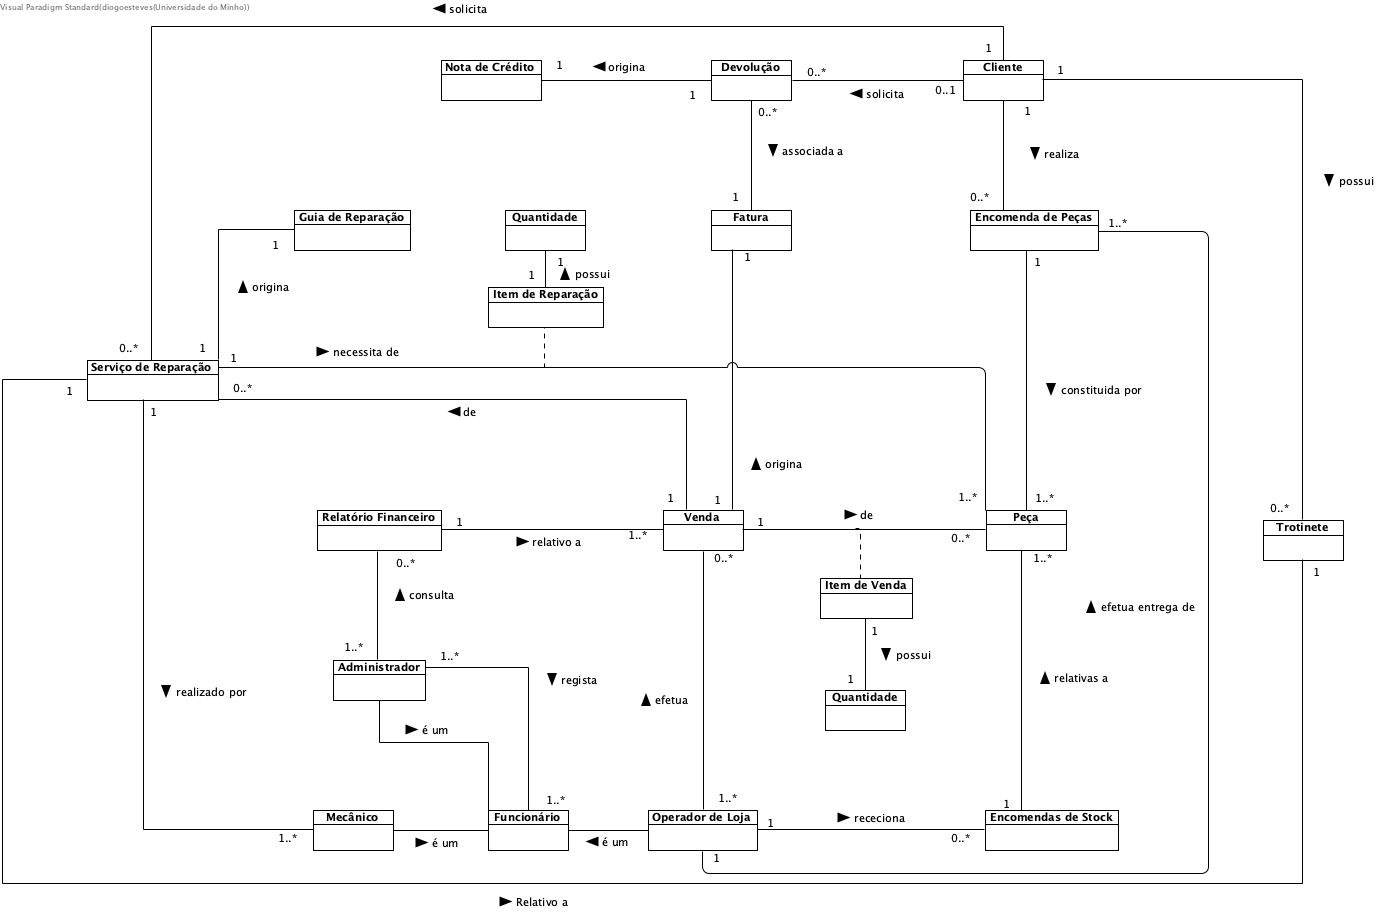
\includegraphics[width=\textwidth, angle=90]{images/Modelo de Domínio.jpg} 
    \caption{Modelo de Domínio (Versão Ampliada)}
\end{figure}

\addsec{Anexo 2 - Log de Prompts}

Neste anexo, listam-se os prompts utilizados para a materialização, estruturação e refinamento da documentação técnica presente neste relatório. Como referido na secção 1.8, a IA atuou como agente auxiliar na redação, partindo sempre de dados e regras de negócio definidos pela equipa técnica. 
% --- Prompt 1 ---
\noindent\textbf{Prompt 1: Contextualização e Visão Estratégica} \\
\textit{Objetivo: Gerar o enquadramento do projeto no panorama das Smart Cities.}
\begin{lstlisting}
"Atua como um Consultor de IT especializado em mobilidade
urbana. Escreve uma contextualização técnica sobre a evolução 
da micromobilidade elétrica na última década e como 
as Smart Cities exigem agora uma digitalização profunda 
dos serviços de assistência técnica."
\end{lstlisting}
\textbf{Resultado:} Secção 1.1.1 (Contextualização).

\vspace{1em}

% --- Prompt 2 ---
\noindent\textbf{Prompt 2: Transformação de Notas em User Stories} \\
\textit{Objetivo: Padronizar as necessidades dos stakeholders recolhidas em entrevistas.}
\begin{lstlisting}
"Com base nos perfis de Administrador, Mecânico e Cliente da 
oficina MobiFix, gera uma lista de User Stories seguindo o
formato: 'Como [ator], quero [ação], para que [benefício]'. 
Garante que cobres os fluxos de agendamento, gestão de stock 
e faturação."
\end{lstlisting}
\textbf{Resultado:} Secção 1.1.8 (User Stories).

\vspace{1em}
% --- Prompt 3 ---
\noindent\textbf{Prompt 3: Refinamento de Requisitos Ambíguos} \\
\textit{Objetivo: Converter linguagem informal em especificações técnicas mensuráveis.}
\begin{lstlisting}
"Refina as seguintes frases de stakeholders para requisitos 
técnicos claros: 
1. 'O sistema deve ser rápido'.
2. 'O cliente deve ser avisado'.
3. 'Controlar melhor o stock'. 
Define métricas como tempos de resposta em segundos e métodos
de notificação."
\end{lstlisting}
\textbf{Resultado:} Tabela 1.2 (Processo de Refinamento e Clarificação).

\vspace{1em}
\newpage
% --- Prompt 4 ---
\noindent\textbf{Prompt 4: Detalhamento de Casos de Uso} \\
\textit{Objetivo: Estruturar o fluxo interativo e condições de exceção para operações críticas.}
\begin{lstlisting}
"Escreve a especificação detalhada do Caso de Uso 'Preencher 
guia de reparacao'. Inclui:
1. Atores envolvidos (Mecanico de Triagem).
2. Pre-condicoes e Pos-condicoes.
3. Fluxo normal de eventos (desde a selecao na agenda ate ao envio de email).
4. Fluxos de excecao (ex: cliente nao concorda com o orcamento)."
\end{lstlisting}
\textbf{Resultado:} Secção 1.3.3 (Tabela 1.37).\vspace{1em}
% --- Prompt 5 ---
\paragraph{}
\noindent\textbf{Prompt 5: Definição da Stack Tecnológica e Restrições} \\
\textit{Objetivo: Estabelecer as diretrizes técnicas de implementação e ambiente operacional.}
\begin{lstlisting}
"Com base num sistema de gestao de oficina web-based, sugere 
uma arquitetura de software multi-tier. Considera o uso de 
.NET para o backend e React.js para o frontend. Define tambem 
as restricoes de persistencia de dados utilizando SQL Server 
e a necessidade de uma interface responsiva com Tailwind CSS."
\end{lstlisting}
\textbf{Resultado:} Secção 1.4 (Especificação do Software).

\vspace{1em}
% --- Prompt 7 ---
\noindent\textbf{Prompt 7: Definicao de Estados e Transicoes} \\
\textit{Objetivo: Mapear o ciclo de vida das entidades para os diagramas de maquina de estados.}
\begin{lstlisting}
"Atua como analista de sistemas. Define os estados possiveis
para uma 'Ordem de Servico' numa oficina de trotinetes, desde
o agendamento ate ao levantamento final. Explica quais os 
eventos que disparam a transicao entre estados (ex: o que 
faz passar de 'Em Execucao' para 'Concluido') para ajudar na 
criacao de um diagrama de estados UML."
\end{lstlisting}
\textbf{Resultado:} Secção 1.7 (Figura 1.17).

\newpage
\vspace{1em}
% --- Prompt 8 ---
\noindent\textbf{Prompt 8: Estruturacao de Indicadores de Desempenho (KPIs)} \\
\textit{Objetivo: Definir a logica para a geracao de relatorios operacionais e financeiros.}
\begin{lstlisting}
"A MobiFix precisa de relatorios mensais para a administracao.
Sugere uma estrutura de dados e formulas para calcular:

Tempo medio de reparacao (Lead Time).

Divisao de faturacao entre pecas e mao-de-obra.

Alerta de pecas com maior volume de saida para otimizacao de 
stock minimo."
\end{lstlisting}
\textbf{Resultado:} Secção 1.2.4 (Requisito Funcional 15 - Tabela 1.17).

\vspace{1em}


\vspace{1.5em}


\end{document}